\section{Odpowiedzi skokowe 12 torów procesów}
\label{projekt:zad2}


Wyznaczono odpowiedzi skokowe dla 12 torów procesu to znaczy zestaw liczb smn dla m równe 1, 2, 3, 
gdzie m oznacza numer wyjścia y i n równe 1, 2, 3, 4, 
gdzie n oznacz numer sterowania u przy pojedynczych skokach jednostkowych odpowiednich sygnałów  sterujących
od chwili k równe 0 włącznie sygnał wymusznia ma wartośc 1, 
w przeszłości jest zerowy.

\begin{figure}[H] 
    \centering
    % This file was created by matlab2tikz.
%
\definecolor{mycolor1}{rgb}{0.00000,0.44700,0.74100}%
%
\begin{tikzpicture}

\begin{axis}[%
width=4.521in,
height=0.944in,
at={(0.758in,3.103in)},
scale only axis,
xmin=0,
xmax=900,
xlabel style={font=\color{white!15!black}},
xlabel={k},
ymin=0,
ymax=4,
ylabel style={font=\color{white!15!black}},
ylabel={$\text{S}^{\text{1,1}}$},
axis background/.style={fill=white},
xmajorgrids,
ymajorgrids,
legend style={legend cell align=left, align=left, draw=white!15!black}
]
\addplot [color=mycolor1]
  table[row sep=crcr]{%
1	3.6291e-06\\
2	1.62e-05\\
3	4.3581e-05\\
4	9.1555e-05\\
5	0.00016548\\
6	0.0002701\\
7	0.00040951\\
8	0.00058711\\
9	0.00080568\\
10	0.0010673\\
11	0.0013737\\
12	0.0017258\\
13	0.0021243\\
14	0.0025695\\
15	0.0030611\\
16	0.0035987\\
17	0.0041816\\
18	0.0048088\\
19	0.0054792\\
20	0.0061914\\
21	0.006944\\
22	0.0077353\\
23	0.0085637\\
24	0.0094273\\
25	0.010324\\
26	0.011253\\
27	0.012211\\
28	0.013198\\
29	0.01421\\
30	0.015246\\
31	0.016303\\
32	0.017382\\
33	0.018478\\
34	0.019591\\
35	0.020719\\
36	0.02186\\
37	0.023012\\
38	0.024174\\
39	0.025344\\
40	0.026521\\
41	0.027703\\
42	0.028888\\
43	0.030077\\
44	0.031266\\
45	0.032455\\
46	0.033644\\
47	0.034829\\
48	0.036012\\
49	0.03719\\
50	0.038362\\
51	0.039529\\
52	0.040688\\
53	0.04184\\
54	0.042983\\
55	0.044117\\
56	0.04524\\
57	0.046354\\
58	0.047456\\
59	0.048547\\
60	0.049625\\
61	0.050691\\
62	0.051745\\
63	0.052785\\
64	0.053811\\
65	0.054824\\
66	0.055822\\
67	0.056807\\
68	0.057776\\
69	0.058732\\
70	0.059672\\
71	0.060597\\
72	0.061507\\
73	0.062403\\
74	0.063283\\
75	0.064148\\
76	0.064997\\
77	0.065832\\
78	0.066651\\
79	0.067456\\
80	0.068245\\
81	0.069019\\
82	0.069778\\
83	0.070523\\
84	0.071252\\
85	0.071967\\
86	0.072668\\
87	0.073354\\
88	0.074026\\
89	0.074684\\
90	0.075328\\
91	0.075959\\
92	0.076575\\
93	0.077179\\
94	0.077769\\
95	0.078346\\
96	0.07891\\
97	0.079461\\
98	0.08\\
99	0.080527\\
100	0.081041\\
101	0.081544\\
102	0.082034\\
103	0.082514\\
104	0.082982\\
105	0.083439\\
106	0.083885\\
107	0.08432\\
108	0.084744\\
109	0.085159\\
110	0.085563\\
111	0.085957\\
112	0.086342\\
113	0.086717\\
114	0.087082\\
115	0.087439\\
116	0.087786\\
117	0.088125\\
118	0.088455\\
119	0.088776\\
120	0.08909\\
121	0.089395\\
122	0.089692\\
123	0.089982\\
124	0.090264\\
125	0.090539\\
126	0.090806\\
127	0.091067\\
128	0.09132\\
129	0.091567\\
130	0.091807\\
131	0.092041\\
132	0.092269\\
133	0.09249\\
134	0.092706\\
135	0.092916\\
136	0.09312\\
137	0.093318\\
138	0.093511\\
139	0.093699\\
140	0.093882\\
141	0.094059\\
142	0.094232\\
143	0.0944\\
144	0.094563\\
145	0.094722\\
146	0.094876\\
147	0.095026\\
148	0.095172\\
149	0.095314\\
150	0.095452\\
151	0.095586\\
152	0.095716\\
153	0.095843\\
154	0.095965\\
155	0.096085\\
156	0.096201\\
157	0.096314\\
158	0.096423\\
159	0.096529\\
160	0.096633\\
161	0.096733\\
162	0.096831\\
163	0.096925\\
164	0.097017\\
165	0.097107\\
166	0.097193\\
167	0.097278\\
168	0.097359\\
169	0.097439\\
170	0.097516\\
171	0.097591\\
172	0.097663\\
173	0.097734\\
174	0.097802\\
175	0.097869\\
176	0.097933\\
177	0.097996\\
178	0.098057\\
179	0.098116\\
180	0.098173\\
181	0.098228\\
182	0.098282\\
183	0.098334\\
184	0.098385\\
185	0.098434\\
186	0.098482\\
187	0.098529\\
188	0.098574\\
189	0.098617\\
190	0.09866\\
191	0.098701\\
192	0.09874\\
193	0.098779\\
194	0.098817\\
195	0.098853\\
196	0.098888\\
197	0.098922\\
198	0.098956\\
199	0.098988\\
200	0.099019\\
201	0.099049\\
202	0.099079\\
203	0.099107\\
204	0.099135\\
205	0.099161\\
206	0.099187\\
207	0.099213\\
208	0.099237\\
209	0.099261\\
210	0.099284\\
211	0.099306\\
212	0.099327\\
213	0.099348\\
214	0.099368\\
215	0.099388\\
216	0.099407\\
217	0.099426\\
218	0.099444\\
219	0.099461\\
220	0.099478\\
221	0.099494\\
222	0.09951\\
223	0.099525\\
224	0.09954\\
225	0.099554\\
226	0.099568\\
227	0.099582\\
228	0.099595\\
229	0.099608\\
230	0.09962\\
231	0.099632\\
232	0.099643\\
233	0.099655\\
234	0.099665\\
235	0.099676\\
236	0.099686\\
237	0.099696\\
238	0.099705\\
239	0.099715\\
240	0.099724\\
241	0.099732\\
242	0.099741\\
243	0.099749\\
244	0.099757\\
245	0.099765\\
246	0.099772\\
247	0.099779\\
248	0.099786\\
249	0.099793\\
250	0.099799\\
251	0.099806\\
252	0.099812\\
253	0.099818\\
254	0.099824\\
255	0.099829\\
256	0.099835\\
257	0.09984\\
258	0.099845\\
259	0.09985\\
260	0.099855\\
261	0.099859\\
262	0.099864\\
263	0.099868\\
264	0.099872\\
265	0.099876\\
266	0.09988\\
267	0.099884\\
268	0.099888\\
269	0.099891\\
270	0.099895\\
271	0.099898\\
272	0.099901\\
273	0.099904\\
274	0.099907\\
275	0.09991\\
276	0.099913\\
277	0.099916\\
278	0.099919\\
279	0.099921\\
280	0.099924\\
281	0.099926\\
282	0.099929\\
283	0.099931\\
284	0.099933\\
285	0.099935\\
286	0.099937\\
287	0.099939\\
288	0.099941\\
289	0.099943\\
290	0.099945\\
291	0.099947\\
292	0.099948\\
293	0.09995\\
294	0.099952\\
295	0.099953\\
296	0.099955\\
297	0.099956\\
298	0.099958\\
299	0.099959\\
300	0.09996\\
301	0.099962\\
302	0.099963\\
303	0.099964\\
304	0.099965\\
305	0.099966\\
306	0.099967\\
307	0.099968\\
308	0.099969\\
309	0.09997\\
310	0.099971\\
311	0.099972\\
312	0.099973\\
313	0.099974\\
314	0.099975\\
315	0.099976\\
316	0.099976\\
317	0.099977\\
318	0.099978\\
319	0.099979\\
320	0.099979\\
321	0.09998\\
322	0.099981\\
323	0.099981\\
324	0.099982\\
325	0.099982\\
326	0.099983\\
327	0.099984\\
328	0.099984\\
329	0.099985\\
330	0.099985\\
331	0.099986\\
332	0.099986\\
333	0.099986\\
334	0.099987\\
335	0.099987\\
336	0.099988\\
337	0.099988\\
338	0.099989\\
339	0.099989\\
340	0.099989\\
341	0.09999\\
342	0.09999\\
343	0.09999\\
344	0.099991\\
345	0.099991\\
346	0.099991\\
347	0.099991\\
348	0.099992\\
349	0.099992\\
350	0.099992\\
351	0.099993\\
352	0.099993\\
353	0.099993\\
354	0.099993\\
355	0.099993\\
356	0.099994\\
357	0.099994\\
358	0.099994\\
359	0.099994\\
360	0.099994\\
361	0.099995\\
362	0.099995\\
363	0.099995\\
364	0.099995\\
365	0.099995\\
366	0.099995\\
367	0.099996\\
368	0.099996\\
369	0.099996\\
370	0.099996\\
371	0.099996\\
372	0.099996\\
373	0.099996\\
374	0.099996\\
375	0.099997\\
376	0.099997\\
377	0.099997\\
378	0.099997\\
379	0.099997\\
380	0.099997\\
381	0.099997\\
382	0.099997\\
383	0.099997\\
384	0.099997\\
385	0.099998\\
386	0.099998\\
387	0.099998\\
388	0.099998\\
389	0.099998\\
390	0.099998\\
391	0.099998\\
392	0.099998\\
393	0.099998\\
394	0.099998\\
395	0.099998\\
396	0.099998\\
397	0.099998\\
398	0.099998\\
399	0.099998\\
400	0.099999\\
401	0.099999\\
402	0.099999\\
403	0.099999\\
404	0.099999\\
405	0.099999\\
406	0.099999\\
407	0.099999\\
408	0.099999\\
409	0.099999\\
410	0.099999\\
411	0.099999\\
412	0.099999\\
413	0.099999\\
414	0.099999\\
415	0.099999\\
416	0.099999\\
417	0.099999\\
418	0.099999\\
419	0.099999\\
420	0.099999\\
421	0.099999\\
422	0.099999\\
423	0.099999\\
424	0.099999\\
425	0.099999\\
426	0.099999\\
427	0.099999\\
428	0.099999\\
429	0.099999\\
430	0.099999\\
431	0.099999\\
432	0.099999\\
433	0.099999\\
434	0.1\\
435	0.1\\
436	0.1\\
437	0.1\\
438	0.1\\
439	0.1\\
440	0.1\\
441	0.1\\
442	0.1\\
443	0.1\\
444	0.1\\
445	0.1\\
446	0.1\\
447	0.1\\
448	0.1\\
449	0.1\\
450	0.1\\
451	0.1\\
452	0.1\\
453	0.1\\
454	0.1\\
455	0.1\\
456	0.1\\
457	0.1\\
458	0.1\\
459	0.1\\
460	0.1\\
461	0.1\\
462	0.1\\
463	0.1\\
464	0.1\\
465	0.1\\
466	0.1\\
467	0.1\\
468	0.1\\
469	0.1\\
470	0.1\\
471	0.1\\
472	0.1\\
473	0.1\\
474	0.1\\
475	0.1\\
476	0.1\\
477	0.1\\
478	0.1\\
479	0.1\\
480	0.1\\
481	0.1\\
482	0.1\\
483	0.1\\
484	0.1\\
485	0.1\\
486	0.1\\
487	0.1\\
488	0.1\\
489	0.1\\
490	0.1\\
491	0.1\\
492	0.1\\
493	0.1\\
494	0.1\\
495	0.1\\
496	0.1\\
497	0.1\\
498	0.1\\
499	0.1\\
500	0.1\\
501	0.1\\
502	0.1\\
503	0.1\\
504	0.1\\
505	0.1\\
506	0.1\\
507	0.1\\
508	0.1\\
509	0.1\\
510	0.1\\
511	0.1\\
512	0.1\\
513	0.1\\
514	0.1\\
515	0.1\\
516	0.1\\
517	0.1\\
518	0.1\\
519	0.1\\
520	0.1\\
521	0.1\\
522	0.1\\
523	0.1\\
524	0.1\\
525	0.1\\
526	0.1\\
527	0.1\\
528	0.1\\
529	0.1\\
530	0.1\\
531	0.1\\
532	0.1\\
533	0.1\\
534	0.1\\
535	0.1\\
536	0.1\\
537	0.1\\
538	0.1\\
539	0.1\\
540	0.1\\
541	0.1\\
542	0.1\\
543	0.1\\
544	0.1\\
545	0.1\\
546	0.1\\
547	0.1\\
548	0.1\\
549	0.1\\
550	0.1\\
551	0.1\\
552	0.1\\
553	0.1\\
554	0.1\\
555	0.1\\
556	0.1\\
557	0.1\\
558	0.1\\
559	0.1\\
560	0.1\\
561	0.1\\
562	0.1\\
563	0.1\\
564	0.1\\
565	0.1\\
566	0.1\\
567	0.1\\
568	0.1\\
569	0.1\\
570	0.1\\
571	0.1\\
572	0.1\\
573	0.1\\
574	0.1\\
575	0.1\\
576	0.1\\
577	0.1\\
578	0.1\\
579	0.1\\
580	0.1\\
581	0.1\\
582	0.1\\
583	0.1\\
584	0.1\\
585	0.1\\
586	0.1\\
587	0.1\\
588	0.1\\
589	0.1\\
590	0.1\\
591	0.1\\
592	0.1\\
593	0.1\\
594	0.1\\
595	0.1\\
596	0.1\\
597	0.1\\
598	0.1\\
599	0.1\\
600	0.1\\
601	0.1\\
602	0.1\\
603	0.1\\
604	0.1\\
605	0.1\\
606	0.1\\
607	0.1\\
608	0.1\\
609	0.1\\
610	0.1\\
611	0.1\\
612	0.1\\
613	0.1\\
614	0.1\\
615	0.1\\
616	0.1\\
617	0.1\\
618	0.1\\
619	0.1\\
620	0.1\\
621	0.1\\
622	0.1\\
623	0.1\\
624	0.1\\
625	0.1\\
626	0.1\\
627	0.1\\
628	0.1\\
629	0.1\\
630	0.1\\
631	0.1\\
632	0.1\\
633	0.1\\
634	0.1\\
635	0.1\\
636	0.1\\
637	0.1\\
638	0.1\\
639	0.1\\
640	0.1\\
641	0.1\\
642	0.1\\
643	0.1\\
644	0.1\\
645	0.1\\
646	0.1\\
647	0.1\\
648	0.1\\
649	0.1\\
650	0.1\\
651	0.1\\
652	0.1\\
653	0.1\\
654	0.1\\
655	0.1\\
656	0.1\\
657	0.1\\
658	0.1\\
659	0.1\\
660	0.1\\
661	0.1\\
662	0.1\\
663	0.1\\
664	0.1\\
665	0.1\\
666	0.1\\
667	0.1\\
668	0.1\\
669	0.1\\
670	0.1\\
671	0.1\\
672	0.1\\
673	0.1\\
674	0.1\\
675	0.1\\
676	0.1\\
677	0.1\\
678	0.1\\
679	0.1\\
680	0.1\\
681	0.1\\
682	0.1\\
683	0.1\\
684	0.1\\
685	0.1\\
686	0.1\\
687	0.1\\
688	0.1\\
689	0.1\\
690	0.1\\
691	0.1\\
692	0.1\\
693	0.1\\
694	0.1\\
695	0.1\\
696	0.1\\
697	0.1\\
698	0.1\\
699	0.1\\
700	0.1\\
701	0.1\\
702	0.1\\
703	0.1\\
704	0.1\\
705	0.1\\
706	0.1\\
707	0.1\\
708	0.1\\
709	0.1\\
710	0.1\\
711	0.1\\
712	0.1\\
713	0.1\\
714	0.1\\
715	0.1\\
716	0.1\\
717	0.1\\
718	0.1\\
719	0.1\\
720	0.1\\
721	0.1\\
722	0.1\\
723	0.1\\
724	0.1\\
725	0.1\\
726	0.1\\
727	0.1\\
728	0.1\\
729	0.1\\
730	0.1\\
731	0.1\\
732	0.1\\
733	0.1\\
734	0.1\\
735	0.1\\
736	0.1\\
737	0.1\\
738	0.1\\
739	0.1\\
740	0.1\\
741	0.1\\
742	0.1\\
743	0.1\\
744	0.1\\
745	0.1\\
746	0.1\\
747	0.1\\
748	0.1\\
749	0.1\\
750	0.1\\
751	0.1\\
752	0.1\\
753	0.1\\
754	0.1\\
755	0.1\\
756	0.1\\
757	0.1\\
758	0.1\\
759	0.1\\
760	0.1\\
761	0.1\\
762	0.1\\
763	0.1\\
764	0.1\\
765	0.1\\
766	0.1\\
767	0.1\\
768	0.1\\
769	0.1\\
770	0.1\\
771	0.1\\
772	0.1\\
773	0.1\\
774	0.1\\
775	0.1\\
776	0.1\\
777	0.1\\
778	0.1\\
779	0.1\\
780	0.1\\
781	0.1\\
782	0.1\\
783	0.1\\
784	0.1\\
785	0.1\\
786	0.1\\
787	0.1\\
788	0.1\\
789	0.1\\
790	0.1\\
791	0.1\\
792	0.1\\
793	0.1\\
794	0.1\\
795	0.1\\
796	0.1\\
797	0.1\\
798	0.1\\
799	0.1\\
800	0.1\\
801	0.1\\
802	0.1\\
803	0.1\\
804	0.1\\
805	0.1\\
806	0.1\\
807	0.1\\
808	0.1\\
809	0.1\\
810	0.1\\
811	0.1\\
812	0.1\\
813	0.1\\
814	0.1\\
815	0.1\\
816	0.1\\
817	0.1\\
818	0.1\\
819	0.1\\
820	0.1\\
821	0.1\\
822	0.1\\
823	0.1\\
824	0.1\\
825	0.1\\
826	0.1\\
827	0.1\\
828	0.1\\
829	0.1\\
830	0.1\\
831	0.1\\
832	0.1\\
833	0.1\\
834	0.1\\
835	0.1\\
836	0.1\\
837	0.1\\
838	0.1\\
839	0.1\\
840	0.1\\
841	0.1\\
842	0.1\\
843	0.1\\
844	0.1\\
845	0.1\\
846	0.1\\
847	0.1\\
848	0.1\\
849	0.1\\
850	0.1\\
851	0.1\\
852	0.1\\
853	0.1\\
854	0.1\\
855	0.1\\
856	0.1\\
857	0.1\\
858	0.1\\
859	0.1\\
860	0.1\\
861	0.1\\
862	0.1\\
863	0.1\\
864	0.1\\
865	0.1\\
866	0.1\\
867	0.1\\
868	0.1\\
869	0.1\\
870	0.1\\
871	0.1\\
872	0.1\\
873	0.1\\
874	0.1\\
875	0.1\\
876	0.1\\
877	0.1\\
878	0.1\\
879	0.1\\
880	0.1\\
881	0.1\\
882	0.1\\
883	0.1\\
884	0.1\\
885	0.1\\
886	0.1\\
887	0.1\\
888	0.1\\
889	0.1\\
890	0.1\\
891	0.1\\
892	0.1\\
893	0.1\\
894	0.1\\
895	0.1\\
896	0.1\\
897	0.1\\
898	0.1\\
899	0.1\\
900	0.1\\
};
\addlegendentry{$\text{S}^\text{1}^\text{,}^\text{1}$}

\end{axis}

\begin{axis}[%
width=4.521in,
height=0.944in,
at={(0.758in,1.792in)},
scale only axis,
xmin=0,
xmax=900,
xlabel style={font=\color{white!15!black}},
xlabel={k},
ymin=0,
ymax=4,
ylabel style={font=\color{white!15!black}},
ylabel={$\text{S}^{\text{2,1}}$},
axis background/.style={fill=white},
xmajorgrids,
ymajorgrids,
legend style={legend cell align=left, align=left, draw=white!15!black}
]
\addplot [color=mycolor1]
  table[row sep=crcr]{%
1	1.3999e-05\\
2	6.3392e-05\\
3	0.00017244\\
4	0.00036526\\
5	0.0006639\\
6	0.0010873\\
7	0.0016505\\
8	0.0023649\\
9	0.003238\\
10	0.0042737\\
11	0.0054727\\
12	0.0068331\\
13	0.0083504\\
14	0.010018\\
15	0.011829\\
16	0.013773\\
17	0.01584\\
18	0.018021\\
19	0.020303\\
20	0.022675\\
21	0.025127\\
22	0.027648\\
23	0.030226\\
24	0.032852\\
25	0.035515\\
26	0.038206\\
27	0.040917\\
28	0.043638\\
29	0.046363\\
30	0.049084\\
31	0.051795\\
32	0.054489\\
33	0.057162\\
34	0.059808\\
35	0.062423\\
36	0.065003\\
37	0.067545\\
38	0.070046\\
39	0.072502\\
40	0.074913\\
41	0.077275\\
42	0.079588\\
43	0.08185\\
44	0.084059\\
45	0.086217\\
46	0.088321\\
47	0.090371\\
48	0.092369\\
49	0.094312\\
50	0.096202\\
51	0.09804\\
52	0.099824\\
53	0.10156\\
54	0.10324\\
55	0.10487\\
56	0.10645\\
57	0.10798\\
58	0.10947\\
59	0.1109\\
60	0.1123\\
61	0.11364\\
62	0.11494\\
63	0.1162\\
64	0.11742\\
65	0.1186\\
66	0.11974\\
67	0.12083\\
68	0.12189\\
69	0.12292\\
70	0.12391\\
71	0.12486\\
72	0.12578\\
73	0.12667\\
74	0.12753\\
75	0.12836\\
76	0.12916\\
77	0.12993\\
78	0.13067\\
79	0.13138\\
80	0.13207\\
81	0.13274\\
82	0.13338\\
83	0.134\\
84	0.13459\\
85	0.13517\\
86	0.13572\\
87	0.13625\\
88	0.13677\\
89	0.13726\\
90	0.13774\\
91	0.13819\\
92	0.13864\\
93	0.13906\\
94	0.13947\\
95	0.13986\\
96	0.14024\\
97	0.14061\\
98	0.14096\\
99	0.1413\\
100	0.14163\\
101	0.14194\\
102	0.14224\\
103	0.14254\\
104	0.14282\\
105	0.14309\\
106	0.14335\\
107	0.1436\\
108	0.14384\\
109	0.14407\\
110	0.14429\\
111	0.14451\\
112	0.14471\\
113	0.14491\\
114	0.1451\\
115	0.14529\\
116	0.14547\\
117	0.14564\\
118	0.1458\\
119	0.14596\\
120	0.14611\\
121	0.14626\\
122	0.1464\\
123	0.14653\\
124	0.14666\\
125	0.14679\\
126	0.14691\\
127	0.14703\\
128	0.14714\\
129	0.14725\\
130	0.14735\\
131	0.14745\\
132	0.14755\\
133	0.14764\\
134	0.14773\\
135	0.14781\\
136	0.1479\\
137	0.14798\\
138	0.14805\\
139	0.14813\\
140	0.1482\\
141	0.14826\\
142	0.14833\\
143	0.14839\\
144	0.14845\\
145	0.14851\\
146	0.14857\\
147	0.14862\\
148	0.14867\\
149	0.14872\\
150	0.14877\\
151	0.14882\\
152	0.14886\\
153	0.14891\\
154	0.14895\\
155	0.14899\\
156	0.14903\\
157	0.14906\\
158	0.1491\\
159	0.14913\\
160	0.14916\\
161	0.1492\\
162	0.14923\\
163	0.14926\\
164	0.14928\\
165	0.14931\\
166	0.14934\\
167	0.14936\\
168	0.14939\\
169	0.14941\\
170	0.14943\\
171	0.14945\\
172	0.14947\\
173	0.14949\\
174	0.14951\\
175	0.14953\\
176	0.14955\\
177	0.14957\\
178	0.14958\\
179	0.1496\\
180	0.14961\\
181	0.14963\\
182	0.14964\\
183	0.14965\\
184	0.14967\\
185	0.14968\\
186	0.14969\\
187	0.1497\\
188	0.14972\\
189	0.14973\\
190	0.14974\\
191	0.14975\\
192	0.14976\\
193	0.14977\\
194	0.14977\\
195	0.14978\\
196	0.14979\\
197	0.1498\\
198	0.14981\\
199	0.14981\\
200	0.14982\\
201	0.14983\\
202	0.14983\\
203	0.14984\\
204	0.14985\\
205	0.14985\\
206	0.14986\\
207	0.14986\\
208	0.14987\\
209	0.14987\\
210	0.14988\\
211	0.14988\\
212	0.14989\\
213	0.14989\\
214	0.1499\\
215	0.1499\\
216	0.1499\\
217	0.14991\\
218	0.14991\\
219	0.14991\\
220	0.14992\\
221	0.14992\\
222	0.14992\\
223	0.14993\\
224	0.14993\\
225	0.14993\\
226	0.14993\\
227	0.14994\\
228	0.14994\\
229	0.14994\\
230	0.14994\\
231	0.14995\\
232	0.14995\\
233	0.14995\\
234	0.14995\\
235	0.14995\\
236	0.14996\\
237	0.14996\\
238	0.14996\\
239	0.14996\\
240	0.14996\\
241	0.14996\\
242	0.14996\\
243	0.14997\\
244	0.14997\\
245	0.14997\\
246	0.14997\\
247	0.14997\\
248	0.14997\\
249	0.14997\\
250	0.14997\\
251	0.14997\\
252	0.14998\\
253	0.14998\\
254	0.14998\\
255	0.14998\\
256	0.14998\\
257	0.14998\\
258	0.14998\\
259	0.14998\\
260	0.14998\\
261	0.14998\\
262	0.14998\\
263	0.14998\\
264	0.14998\\
265	0.14999\\
266	0.14999\\
267	0.14999\\
268	0.14999\\
269	0.14999\\
270	0.14999\\
271	0.14999\\
272	0.14999\\
273	0.14999\\
274	0.14999\\
275	0.14999\\
276	0.14999\\
277	0.14999\\
278	0.14999\\
279	0.14999\\
280	0.14999\\
281	0.14999\\
282	0.14999\\
283	0.14999\\
284	0.14999\\
285	0.14999\\
286	0.14999\\
287	0.14999\\
288	0.14999\\
289	0.14999\\
290	0.14999\\
291	0.14999\\
292	0.14999\\
293	0.14999\\
294	0.15\\
295	0.15\\
296	0.15\\
297	0.15\\
298	0.15\\
299	0.15\\
300	0.15\\
301	0.15\\
302	0.15\\
303	0.15\\
304	0.15\\
305	0.15\\
306	0.15\\
307	0.15\\
308	0.15\\
309	0.15\\
310	0.15\\
311	0.15\\
312	0.15\\
313	0.15\\
314	0.15\\
315	0.15\\
316	0.15\\
317	0.15\\
318	0.15\\
319	0.15\\
320	0.15\\
321	0.15\\
322	0.15\\
323	0.15\\
324	0.15\\
325	0.15\\
326	0.15\\
327	0.15\\
328	0.15\\
329	0.15\\
330	0.15\\
331	0.15\\
332	0.15\\
333	0.15\\
334	0.15\\
335	0.15\\
336	0.15\\
337	0.15\\
338	0.15\\
339	0.15\\
340	0.15\\
341	0.15\\
342	0.15\\
343	0.15\\
344	0.15\\
345	0.15\\
346	0.15\\
347	0.15\\
348	0.15\\
349	0.15\\
350	0.15\\
351	0.15\\
352	0.15\\
353	0.15\\
354	0.15\\
355	0.15\\
356	0.15\\
357	0.15\\
358	0.15\\
359	0.15\\
360	0.15\\
361	0.15\\
362	0.15\\
363	0.15\\
364	0.15\\
365	0.15\\
366	0.15\\
367	0.15\\
368	0.15\\
369	0.15\\
370	0.15\\
371	0.15\\
372	0.15\\
373	0.15\\
374	0.15\\
375	0.15\\
376	0.15\\
377	0.15\\
378	0.15\\
379	0.15\\
380	0.15\\
381	0.15\\
382	0.15\\
383	0.15\\
384	0.15\\
385	0.15\\
386	0.15\\
387	0.15\\
388	0.15\\
389	0.15\\
390	0.15\\
391	0.15\\
392	0.15\\
393	0.15\\
394	0.15\\
395	0.15\\
396	0.15\\
397	0.15\\
398	0.15\\
399	0.15\\
400	0.15\\
401	0.15\\
402	0.15\\
403	0.15\\
404	0.15\\
405	0.15\\
406	0.15\\
407	0.15\\
408	0.15\\
409	0.15\\
410	0.15\\
411	0.15\\
412	0.15\\
413	0.15\\
414	0.15\\
415	0.15\\
416	0.15\\
417	0.15\\
418	0.15\\
419	0.15\\
420	0.15\\
421	0.15\\
422	0.15\\
423	0.15\\
424	0.15\\
425	0.15\\
426	0.15\\
427	0.15\\
428	0.15\\
429	0.15\\
430	0.15\\
431	0.15\\
432	0.15\\
433	0.15\\
434	0.15\\
435	0.15\\
436	0.15\\
437	0.15\\
438	0.15\\
439	0.15\\
440	0.15\\
441	0.15\\
442	0.15\\
443	0.15\\
444	0.15\\
445	0.15\\
446	0.15\\
447	0.15\\
448	0.15\\
449	0.15\\
450	0.15\\
451	0.15\\
452	0.15\\
453	0.15\\
454	0.15\\
455	0.15\\
456	0.15\\
457	0.15\\
458	0.15\\
459	0.15\\
460	0.15\\
461	0.15\\
462	0.15\\
463	0.15\\
464	0.15\\
465	0.15\\
466	0.15\\
467	0.15\\
468	0.15\\
469	0.15\\
470	0.15\\
471	0.15\\
472	0.15\\
473	0.15\\
474	0.15\\
475	0.15\\
476	0.15\\
477	0.15\\
478	0.15\\
479	0.15\\
480	0.15\\
481	0.15\\
482	0.15\\
483	0.15\\
484	0.15\\
485	0.15\\
486	0.15\\
487	0.15\\
488	0.15\\
489	0.15\\
490	0.15\\
491	0.15\\
492	0.15\\
493	0.15\\
494	0.15\\
495	0.15\\
496	0.15\\
497	0.15\\
498	0.15\\
499	0.15\\
500	0.15\\
501	0.15\\
502	0.15\\
503	0.15\\
504	0.15\\
505	0.15\\
506	0.15\\
507	0.15\\
508	0.15\\
509	0.15\\
510	0.15\\
511	0.15\\
512	0.15\\
513	0.15\\
514	0.15\\
515	0.15\\
516	0.15\\
517	0.15\\
518	0.15\\
519	0.15\\
520	0.15\\
521	0.15\\
522	0.15\\
523	0.15\\
524	0.15\\
525	0.15\\
526	0.15\\
527	0.15\\
528	0.15\\
529	0.15\\
530	0.15\\
531	0.15\\
532	0.15\\
533	0.15\\
534	0.15\\
535	0.15\\
536	0.15\\
537	0.15\\
538	0.15\\
539	0.15\\
540	0.15\\
541	0.15\\
542	0.15\\
543	0.15\\
544	0.15\\
545	0.15\\
546	0.15\\
547	0.15\\
548	0.15\\
549	0.15\\
550	0.15\\
551	0.15\\
552	0.15\\
553	0.15\\
554	0.15\\
555	0.15\\
556	0.15\\
557	0.15\\
558	0.15\\
559	0.15\\
560	0.15\\
561	0.15\\
562	0.15\\
563	0.15\\
564	0.15\\
565	0.15\\
566	0.15\\
567	0.15\\
568	0.15\\
569	0.15\\
570	0.15\\
571	0.15\\
572	0.15\\
573	0.15\\
574	0.15\\
575	0.15\\
576	0.15\\
577	0.15\\
578	0.15\\
579	0.15\\
580	0.15\\
581	0.15\\
582	0.15\\
583	0.15\\
584	0.15\\
585	0.15\\
586	0.15\\
587	0.15\\
588	0.15\\
589	0.15\\
590	0.15\\
591	0.15\\
592	0.15\\
593	0.15\\
594	0.15\\
595	0.15\\
596	0.15\\
597	0.15\\
598	0.15\\
599	0.15\\
600	0.15\\
601	0.15\\
602	0.15\\
603	0.15\\
604	0.15\\
605	0.15\\
606	0.15\\
607	0.15\\
608	0.15\\
609	0.15\\
610	0.15\\
611	0.15\\
612	0.15\\
613	0.15\\
614	0.15\\
615	0.15\\
616	0.15\\
617	0.15\\
618	0.15\\
619	0.15\\
620	0.15\\
621	0.15\\
622	0.15\\
623	0.15\\
624	0.15\\
625	0.15\\
626	0.15\\
627	0.15\\
628	0.15\\
629	0.15\\
630	0.15\\
631	0.15\\
632	0.15\\
633	0.15\\
634	0.15\\
635	0.15\\
636	0.15\\
637	0.15\\
638	0.15\\
639	0.15\\
640	0.15\\
641	0.15\\
642	0.15\\
643	0.15\\
644	0.15\\
645	0.15\\
646	0.15\\
647	0.15\\
648	0.15\\
649	0.15\\
650	0.15\\
651	0.15\\
652	0.15\\
653	0.15\\
654	0.15\\
655	0.15\\
656	0.15\\
657	0.15\\
658	0.15\\
659	0.15\\
660	0.15\\
661	0.15\\
662	0.15\\
663	0.15\\
664	0.15\\
665	0.15\\
666	0.15\\
667	0.15\\
668	0.15\\
669	0.15\\
670	0.15\\
671	0.15\\
672	0.15\\
673	0.15\\
674	0.15\\
675	0.15\\
676	0.15\\
677	0.15\\
678	0.15\\
679	0.15\\
680	0.15\\
681	0.15\\
682	0.15\\
683	0.15\\
684	0.15\\
685	0.15\\
686	0.15\\
687	0.15\\
688	0.15\\
689	0.15\\
690	0.15\\
691	0.15\\
692	0.15\\
693	0.15\\
694	0.15\\
695	0.15\\
696	0.15\\
697	0.15\\
698	0.15\\
699	0.15\\
700	0.15\\
701	0.15\\
702	0.15\\
703	0.15\\
704	0.15\\
705	0.15\\
706	0.15\\
707	0.15\\
708	0.15\\
709	0.15\\
710	0.15\\
711	0.15\\
712	0.15\\
713	0.15\\
714	0.15\\
715	0.15\\
716	0.15\\
717	0.15\\
718	0.15\\
719	0.15\\
720	0.15\\
721	0.15\\
722	0.15\\
723	0.15\\
724	0.15\\
725	0.15\\
726	0.15\\
727	0.15\\
728	0.15\\
729	0.15\\
730	0.15\\
731	0.15\\
732	0.15\\
733	0.15\\
734	0.15\\
735	0.15\\
736	0.15\\
737	0.15\\
738	0.15\\
739	0.15\\
740	0.15\\
741	0.15\\
742	0.15\\
743	0.15\\
744	0.15\\
745	0.15\\
746	0.15\\
747	0.15\\
748	0.15\\
749	0.15\\
750	0.15\\
751	0.15\\
752	0.15\\
753	0.15\\
754	0.15\\
755	0.15\\
756	0.15\\
757	0.15\\
758	0.15\\
759	0.15\\
760	0.15\\
761	0.15\\
762	0.15\\
763	0.15\\
764	0.15\\
765	0.15\\
766	0.15\\
767	0.15\\
768	0.15\\
769	0.15\\
770	0.15\\
771	0.15\\
772	0.15\\
773	0.15\\
774	0.15\\
775	0.15\\
776	0.15\\
777	0.15\\
778	0.15\\
779	0.15\\
780	0.15\\
781	0.15\\
782	0.15\\
783	0.15\\
784	0.15\\
785	0.15\\
786	0.15\\
787	0.15\\
788	0.15\\
789	0.15\\
790	0.15\\
791	0.15\\
792	0.15\\
793	0.15\\
794	0.15\\
795	0.15\\
796	0.15\\
797	0.15\\
798	0.15\\
799	0.15\\
800	0.15\\
801	0.15\\
802	0.15\\
803	0.15\\
804	0.15\\
805	0.15\\
806	0.15\\
807	0.15\\
808	0.15\\
809	0.15\\
810	0.15\\
811	0.15\\
812	0.15\\
813	0.15\\
814	0.15\\
815	0.15\\
816	0.15\\
817	0.15\\
818	0.15\\
819	0.15\\
820	0.15\\
821	0.15\\
822	0.15\\
823	0.15\\
824	0.15\\
825	0.15\\
826	0.15\\
827	0.15\\
828	0.15\\
829	0.15\\
830	0.15\\
831	0.15\\
832	0.15\\
833	0.15\\
834	0.15\\
835	0.15\\
836	0.15\\
837	0.15\\
838	0.15\\
839	0.15\\
840	0.15\\
841	0.15\\
842	0.15\\
843	0.15\\
844	0.15\\
845	0.15\\
846	0.15\\
847	0.15\\
848	0.15\\
849	0.15\\
850	0.15\\
851	0.15\\
852	0.15\\
853	0.15\\
854	0.15\\
855	0.15\\
856	0.15\\
857	0.15\\
858	0.15\\
859	0.15\\
860	0.15\\
861	0.15\\
862	0.15\\
863	0.15\\
864	0.15\\
865	0.15\\
866	0.15\\
867	0.15\\
868	0.15\\
869	0.15\\
870	0.15\\
871	0.15\\
872	0.15\\
873	0.15\\
874	0.15\\
875	0.15\\
876	0.15\\
877	0.15\\
878	0.15\\
879	0.15\\
880	0.15\\
881	0.15\\
882	0.15\\
883	0.15\\
884	0.15\\
885	0.15\\
886	0.15\\
887	0.15\\
888	0.15\\
889	0.15\\
890	0.15\\
891	0.15\\
892	0.15\\
893	0.15\\
894	0.15\\
895	0.15\\
896	0.15\\
897	0.15\\
898	0.15\\
899	0.15\\
900	0.15\\
};
\addlegendentry{$\text{S}^{\text{2,1}}$}

\end{axis}

\begin{axis}[%
width=4.521in,
height=0.944in,
at={(0.758in,0.481in)},
scale only axis,
xmin=0,
xmax=900,
xlabel style={font=\color{white!15!black}},
xlabel={k},
ymin=0,
ymax=4,
ylabel style={font=\color{white!15!black}},
ylabel={$\text{S}^{\text{3,1}}$},
axis background/.style={fill=white},
xmajorgrids,
ymajorgrids,
legend style={legend cell align=left, align=left, draw=white!15!black}
]
\addplot [color=mycolor1]
  table[row sep=crcr]{%
1	0.00067918\\
2	0.0025323\\
3	0.0057604\\
4	0.010348\\
5	0.016158\\
6	0.023\\
7	0.03067\\
8	0.03898\\
9	0.047761\\
10	0.056872\\
11	0.066194\\
12	0.075633\\
13	0.085114\\
14	0.094577\\
15	0.10398\\
16	0.11328\\
17	0.12245\\
18	0.13149\\
19	0.14036\\
20	0.14906\\
21	0.15759\\
22	0.16593\\
23	0.1741\\
24	0.18208\\
25	0.18988\\
26	0.1975\\
27	0.20493\\
28	0.2122\\
29	0.21928\\
30	0.2262\\
31	0.23295\\
32	0.23953\\
33	0.24596\\
34	0.25222\\
35	0.25834\\
36	0.2643\\
37	0.27012\\
38	0.27579\\
39	0.28133\\
40	0.28672\\
41	0.29199\\
42	0.29712\\
43	0.30213\\
44	0.30702\\
45	0.31178\\
46	0.31643\\
47	0.32096\\
48	0.32538\\
49	0.32969\\
50	0.3339\\
51	0.338\\
52	0.342\\
53	0.3459\\
54	0.3497\\
55	0.35341\\
56	0.35703\\
57	0.36056\\
58	0.36401\\
59	0.36736\\
60	0.37064\\
61	0.37383\\
62	0.37695\\
63	0.37999\\
64	0.38295\\
65	0.38584\\
66	0.38866\\
67	0.39141\\
68	0.39409\\
69	0.3967\\
70	0.39925\\
71	0.40174\\
72	0.40417\\
73	0.40653\\
74	0.40884\\
75	0.41109\\
76	0.41329\\
77	0.41543\\
78	0.41752\\
79	0.41955\\
80	0.42154\\
81	0.42348\\
82	0.42536\\
83	0.42721\\
84	0.429\\
85	0.43076\\
86	0.43247\\
87	0.43413\\
88	0.43576\\
89	0.43735\\
90	0.43889\\
91	0.4404\\
92	0.44187\\
93	0.44331\\
94	0.44471\\
95	0.44607\\
96	0.44741\\
97	0.4487\\
98	0.44997\\
99	0.45121\\
100	0.45241\\
101	0.45359\\
102	0.45473\\
103	0.45585\\
104	0.45694\\
105	0.458\\
106	0.45904\\
107	0.46005\\
108	0.46104\\
109	0.462\\
110	0.46294\\
111	0.46385\\
112	0.46474\\
113	0.46562\\
114	0.46646\\
115	0.46729\\
116	0.4681\\
117	0.46889\\
118	0.46966\\
119	0.4704\\
120	0.47114\\
121	0.47185\\
122	0.47254\\
123	0.47322\\
124	0.47388\\
125	0.47453\\
126	0.47516\\
127	0.47577\\
128	0.47637\\
129	0.47695\\
130	0.47752\\
131	0.47808\\
132	0.47862\\
133	0.47914\\
134	0.47966\\
135	0.48016\\
136	0.48065\\
137	0.48113\\
138	0.4816\\
139	0.48205\\
140	0.48249\\
141	0.48293\\
142	0.48335\\
143	0.48376\\
144	0.48416\\
145	0.48455\\
146	0.48493\\
147	0.4853\\
148	0.48567\\
149	0.48602\\
150	0.48637\\
151	0.4867\\
152	0.48703\\
153	0.48735\\
154	0.48766\\
155	0.48797\\
156	0.48826\\
157	0.48855\\
158	0.48884\\
159	0.48911\\
160	0.48938\\
161	0.48964\\
162	0.4899\\
163	0.49015\\
164	0.49039\\
165	0.49063\\
166	0.49086\\
167	0.49109\\
168	0.49131\\
169	0.49152\\
170	0.49173\\
171	0.49193\\
172	0.49213\\
173	0.49233\\
174	0.49252\\
175	0.4927\\
176	0.49288\\
177	0.49306\\
178	0.49323\\
179	0.4934\\
180	0.49356\\
181	0.49372\\
182	0.49387\\
183	0.49402\\
184	0.49417\\
185	0.49432\\
186	0.49446\\
187	0.49459\\
188	0.49473\\
189	0.49486\\
190	0.49498\\
191	0.49511\\
192	0.49523\\
193	0.49535\\
194	0.49546\\
195	0.49557\\
196	0.49568\\
197	0.49579\\
198	0.49589\\
199	0.49599\\
200	0.49609\\
201	0.49619\\
202	0.49628\\
203	0.49638\\
204	0.49647\\
205	0.49655\\
206	0.49664\\
207	0.49672\\
208	0.4968\\
209	0.49688\\
210	0.49696\\
211	0.49703\\
212	0.49711\\
213	0.49718\\
214	0.49725\\
215	0.49732\\
216	0.49738\\
217	0.49745\\
218	0.49751\\
219	0.49757\\
220	0.49763\\
221	0.49769\\
222	0.49775\\
223	0.4978\\
224	0.49786\\
225	0.49791\\
226	0.49796\\
227	0.49801\\
228	0.49806\\
229	0.49811\\
230	0.49815\\
231	0.4982\\
232	0.49824\\
233	0.49829\\
234	0.49833\\
235	0.49837\\
236	0.49841\\
237	0.49845\\
238	0.49849\\
239	0.49853\\
240	0.49856\\
241	0.4986\\
242	0.49863\\
243	0.49867\\
244	0.4987\\
245	0.49873\\
246	0.49876\\
247	0.49879\\
248	0.49882\\
249	0.49885\\
250	0.49888\\
251	0.49891\\
252	0.49894\\
253	0.49896\\
254	0.49899\\
255	0.49901\\
256	0.49904\\
257	0.49906\\
258	0.49908\\
259	0.49911\\
260	0.49913\\
261	0.49915\\
262	0.49917\\
263	0.49919\\
264	0.49921\\
265	0.49923\\
266	0.49925\\
267	0.49927\\
268	0.49929\\
269	0.4993\\
270	0.49932\\
271	0.49934\\
272	0.49935\\
273	0.49937\\
274	0.49939\\
275	0.4994\\
276	0.49942\\
277	0.49943\\
278	0.49944\\
279	0.49946\\
280	0.49947\\
281	0.49948\\
282	0.4995\\
283	0.49951\\
284	0.49952\\
285	0.49953\\
286	0.49954\\
287	0.49956\\
288	0.49957\\
289	0.49958\\
290	0.49959\\
291	0.4996\\
292	0.49961\\
293	0.49962\\
294	0.49963\\
295	0.49964\\
296	0.49965\\
297	0.49965\\
298	0.49966\\
299	0.49967\\
300	0.49968\\
301	0.49969\\
302	0.49969\\
303	0.4997\\
304	0.49971\\
305	0.49972\\
306	0.49972\\
307	0.49973\\
308	0.49974\\
309	0.49974\\
310	0.49975\\
311	0.49976\\
312	0.49976\\
313	0.49977\\
314	0.49977\\
315	0.49978\\
316	0.49979\\
317	0.49979\\
318	0.4998\\
319	0.4998\\
320	0.49981\\
321	0.49981\\
322	0.49981\\
323	0.49982\\
324	0.49982\\
325	0.49983\\
326	0.49983\\
327	0.49984\\
328	0.49984\\
329	0.49984\\
330	0.49985\\
331	0.49985\\
332	0.49986\\
333	0.49986\\
334	0.49986\\
335	0.49987\\
336	0.49987\\
337	0.49987\\
338	0.49988\\
339	0.49988\\
340	0.49988\\
341	0.49988\\
342	0.49989\\
343	0.49989\\
344	0.49989\\
345	0.4999\\
346	0.4999\\
347	0.4999\\
348	0.4999\\
349	0.49991\\
350	0.49991\\
351	0.49991\\
352	0.49991\\
353	0.49991\\
354	0.49992\\
355	0.49992\\
356	0.49992\\
357	0.49992\\
358	0.49992\\
359	0.49993\\
360	0.49993\\
361	0.49993\\
362	0.49993\\
363	0.49993\\
364	0.49994\\
365	0.49994\\
366	0.49994\\
367	0.49994\\
368	0.49994\\
369	0.49994\\
370	0.49994\\
371	0.49995\\
372	0.49995\\
373	0.49995\\
374	0.49995\\
375	0.49995\\
376	0.49995\\
377	0.49995\\
378	0.49995\\
379	0.49996\\
380	0.49996\\
381	0.49996\\
382	0.49996\\
383	0.49996\\
384	0.49996\\
385	0.49996\\
386	0.49996\\
387	0.49996\\
388	0.49996\\
389	0.49997\\
390	0.49997\\
391	0.49997\\
392	0.49997\\
393	0.49997\\
394	0.49997\\
395	0.49997\\
396	0.49997\\
397	0.49997\\
398	0.49997\\
399	0.49997\\
400	0.49997\\
401	0.49997\\
402	0.49997\\
403	0.49998\\
404	0.49998\\
405	0.49998\\
406	0.49998\\
407	0.49998\\
408	0.49998\\
409	0.49998\\
410	0.49998\\
411	0.49998\\
412	0.49998\\
413	0.49998\\
414	0.49998\\
415	0.49998\\
416	0.49998\\
417	0.49998\\
418	0.49998\\
419	0.49998\\
420	0.49998\\
421	0.49998\\
422	0.49998\\
423	0.49999\\
424	0.49999\\
425	0.49999\\
426	0.49999\\
427	0.49999\\
428	0.49999\\
429	0.49999\\
430	0.49999\\
431	0.49999\\
432	0.49999\\
433	0.49999\\
434	0.49999\\
435	0.49999\\
436	0.49999\\
437	0.49999\\
438	0.49999\\
439	0.49999\\
440	0.49999\\
441	0.49999\\
442	0.49999\\
443	0.49999\\
444	0.49999\\
445	0.49999\\
446	0.49999\\
447	0.49999\\
448	0.49999\\
449	0.49999\\
450	0.49999\\
451	0.49999\\
452	0.49999\\
453	0.49999\\
454	0.49999\\
455	0.49999\\
456	0.49999\\
457	0.49999\\
458	0.49999\\
459	0.49999\\
460	0.49999\\
461	0.49999\\
462	0.49999\\
463	0.49999\\
464	0.49999\\
465	0.49999\\
466	0.49999\\
467	0.5\\
468	0.5\\
469	0.5\\
470	0.5\\
471	0.5\\
472	0.5\\
473	0.5\\
474	0.5\\
475	0.5\\
476	0.5\\
477	0.5\\
478	0.5\\
479	0.5\\
480	0.5\\
481	0.5\\
482	0.5\\
483	0.5\\
484	0.5\\
485	0.5\\
486	0.5\\
487	0.5\\
488	0.5\\
489	0.5\\
490	0.5\\
491	0.5\\
492	0.5\\
493	0.5\\
494	0.5\\
495	0.5\\
496	0.5\\
497	0.5\\
498	0.5\\
499	0.5\\
500	0.5\\
501	0.5\\
502	0.5\\
503	0.5\\
504	0.5\\
505	0.5\\
506	0.5\\
507	0.5\\
508	0.5\\
509	0.5\\
510	0.5\\
511	0.5\\
512	0.5\\
513	0.5\\
514	0.5\\
515	0.5\\
516	0.5\\
517	0.5\\
518	0.5\\
519	0.5\\
520	0.5\\
521	0.5\\
522	0.5\\
523	0.5\\
524	0.5\\
525	0.5\\
526	0.5\\
527	0.5\\
528	0.5\\
529	0.5\\
530	0.5\\
531	0.5\\
532	0.5\\
533	0.5\\
534	0.5\\
535	0.5\\
536	0.5\\
537	0.5\\
538	0.5\\
539	0.5\\
540	0.5\\
541	0.5\\
542	0.5\\
543	0.5\\
544	0.5\\
545	0.5\\
546	0.5\\
547	0.5\\
548	0.5\\
549	0.5\\
550	0.5\\
551	0.5\\
552	0.5\\
553	0.5\\
554	0.5\\
555	0.5\\
556	0.5\\
557	0.5\\
558	0.5\\
559	0.5\\
560	0.5\\
561	0.5\\
562	0.5\\
563	0.5\\
564	0.5\\
565	0.5\\
566	0.5\\
567	0.5\\
568	0.5\\
569	0.5\\
570	0.5\\
571	0.5\\
572	0.5\\
573	0.5\\
574	0.5\\
575	0.5\\
576	0.5\\
577	0.5\\
578	0.5\\
579	0.5\\
580	0.5\\
581	0.5\\
582	0.5\\
583	0.5\\
584	0.5\\
585	0.5\\
586	0.5\\
587	0.5\\
588	0.5\\
589	0.5\\
590	0.5\\
591	0.5\\
592	0.5\\
593	0.5\\
594	0.5\\
595	0.5\\
596	0.5\\
597	0.5\\
598	0.5\\
599	0.5\\
600	0.5\\
601	0.5\\
602	0.5\\
603	0.5\\
604	0.5\\
605	0.5\\
606	0.5\\
607	0.5\\
608	0.5\\
609	0.5\\
610	0.5\\
611	0.5\\
612	0.5\\
613	0.5\\
614	0.5\\
615	0.5\\
616	0.5\\
617	0.5\\
618	0.5\\
619	0.5\\
620	0.5\\
621	0.5\\
622	0.5\\
623	0.5\\
624	0.5\\
625	0.5\\
626	0.5\\
627	0.5\\
628	0.5\\
629	0.5\\
630	0.5\\
631	0.5\\
632	0.5\\
633	0.5\\
634	0.5\\
635	0.5\\
636	0.5\\
637	0.5\\
638	0.5\\
639	0.5\\
640	0.5\\
641	0.5\\
642	0.5\\
643	0.5\\
644	0.5\\
645	0.5\\
646	0.5\\
647	0.5\\
648	0.5\\
649	0.5\\
650	0.5\\
651	0.5\\
652	0.5\\
653	0.5\\
654	0.5\\
655	0.5\\
656	0.5\\
657	0.5\\
658	0.5\\
659	0.5\\
660	0.5\\
661	0.5\\
662	0.5\\
663	0.5\\
664	0.5\\
665	0.5\\
666	0.5\\
667	0.5\\
668	0.5\\
669	0.5\\
670	0.5\\
671	0.5\\
672	0.5\\
673	0.5\\
674	0.5\\
675	0.5\\
676	0.5\\
677	0.5\\
678	0.5\\
679	0.5\\
680	0.5\\
681	0.5\\
682	0.5\\
683	0.5\\
684	0.5\\
685	0.5\\
686	0.5\\
687	0.5\\
688	0.5\\
689	0.5\\
690	0.5\\
691	0.5\\
692	0.5\\
693	0.5\\
694	0.5\\
695	0.5\\
696	0.5\\
697	0.5\\
698	0.5\\
699	0.5\\
700	0.5\\
701	0.5\\
702	0.5\\
703	0.5\\
704	0.5\\
705	0.5\\
706	0.5\\
707	0.5\\
708	0.5\\
709	0.5\\
710	0.5\\
711	0.5\\
712	0.5\\
713	0.5\\
714	0.5\\
715	0.5\\
716	0.5\\
717	0.5\\
718	0.5\\
719	0.5\\
720	0.5\\
721	0.5\\
722	0.5\\
723	0.5\\
724	0.5\\
725	0.5\\
726	0.5\\
727	0.5\\
728	0.5\\
729	0.5\\
730	0.5\\
731	0.5\\
732	0.5\\
733	0.5\\
734	0.5\\
735	0.5\\
736	0.5\\
737	0.5\\
738	0.5\\
739	0.5\\
740	0.5\\
741	0.5\\
742	0.5\\
743	0.5\\
744	0.5\\
745	0.5\\
746	0.5\\
747	0.5\\
748	0.5\\
749	0.5\\
750	0.5\\
751	0.5\\
752	0.5\\
753	0.5\\
754	0.5\\
755	0.5\\
756	0.5\\
757	0.5\\
758	0.5\\
759	0.5\\
760	0.5\\
761	0.5\\
762	0.5\\
763	0.5\\
764	0.5\\
765	0.5\\
766	0.5\\
767	0.5\\
768	0.5\\
769	0.5\\
770	0.5\\
771	0.5\\
772	0.5\\
773	0.5\\
774	0.5\\
775	0.5\\
776	0.5\\
777	0.5\\
778	0.5\\
779	0.5\\
780	0.5\\
781	0.5\\
782	0.5\\
783	0.5\\
784	0.5\\
785	0.5\\
786	0.5\\
787	0.5\\
788	0.5\\
789	0.5\\
790	0.5\\
791	0.5\\
792	0.5\\
793	0.5\\
794	0.5\\
795	0.5\\
796	0.5\\
797	0.5\\
798	0.5\\
799	0.5\\
800	0.5\\
801	0.5\\
802	0.5\\
803	0.5\\
804	0.5\\
805	0.5\\
806	0.5\\
807	0.5\\
808	0.5\\
809	0.5\\
810	0.5\\
811	0.5\\
812	0.5\\
813	0.5\\
814	0.5\\
815	0.5\\
816	0.5\\
817	0.5\\
818	0.5\\
819	0.5\\
820	0.5\\
821	0.5\\
822	0.5\\
823	0.5\\
824	0.5\\
825	0.5\\
826	0.5\\
827	0.5\\
828	0.5\\
829	0.5\\
830	0.5\\
831	0.5\\
832	0.5\\
833	0.5\\
834	0.5\\
835	0.5\\
836	0.5\\
837	0.5\\
838	0.5\\
839	0.5\\
840	0.5\\
841	0.5\\
842	0.5\\
843	0.5\\
844	0.5\\
845	0.5\\
846	0.5\\
847	0.5\\
848	0.5\\
849	0.5\\
850	0.5\\
851	0.5\\
852	0.5\\
853	0.5\\
854	0.5\\
855	0.5\\
856	0.5\\
857	0.5\\
858	0.5\\
859	0.5\\
860	0.5\\
861	0.5\\
862	0.5\\
863	0.5\\
864	0.5\\
865	0.5\\
866	0.5\\
867	0.5\\
868	0.5\\
869	0.5\\
870	0.5\\
871	0.5\\
872	0.5\\
873	0.5\\
874	0.5\\
875	0.5\\
876	0.5\\
877	0.5\\
878	0.5\\
879	0.5\\
880	0.5\\
881	0.5\\
882	0.5\\
883	0.5\\
884	0.5\\
885	0.5\\
886	0.5\\
887	0.5\\
888	0.5\\
889	0.5\\
890	0.5\\
891	0.5\\
892	0.5\\
893	0.5\\
894	0.5\\
895	0.5\\
896	0.5\\
897	0.5\\
898	0.5\\
899	0.5\\
900	0.5\\
};
\addlegendentry{$\text{S}^{\text{3,1}}$}

\end{axis}
\end{tikzpicture}%
    \caption{projekt-zadanie2-u1-proj-zadanie2u1}
    \label{projekt:zad2:figure:projzadanie2u1}
 \end{figure}

 \begin{figure}[H] 
     \centering
     % This file was created by matlab2tikz.
%
\definecolor{mycolor1}{rgb}{0.00000,0.44700,0.74100}%
%
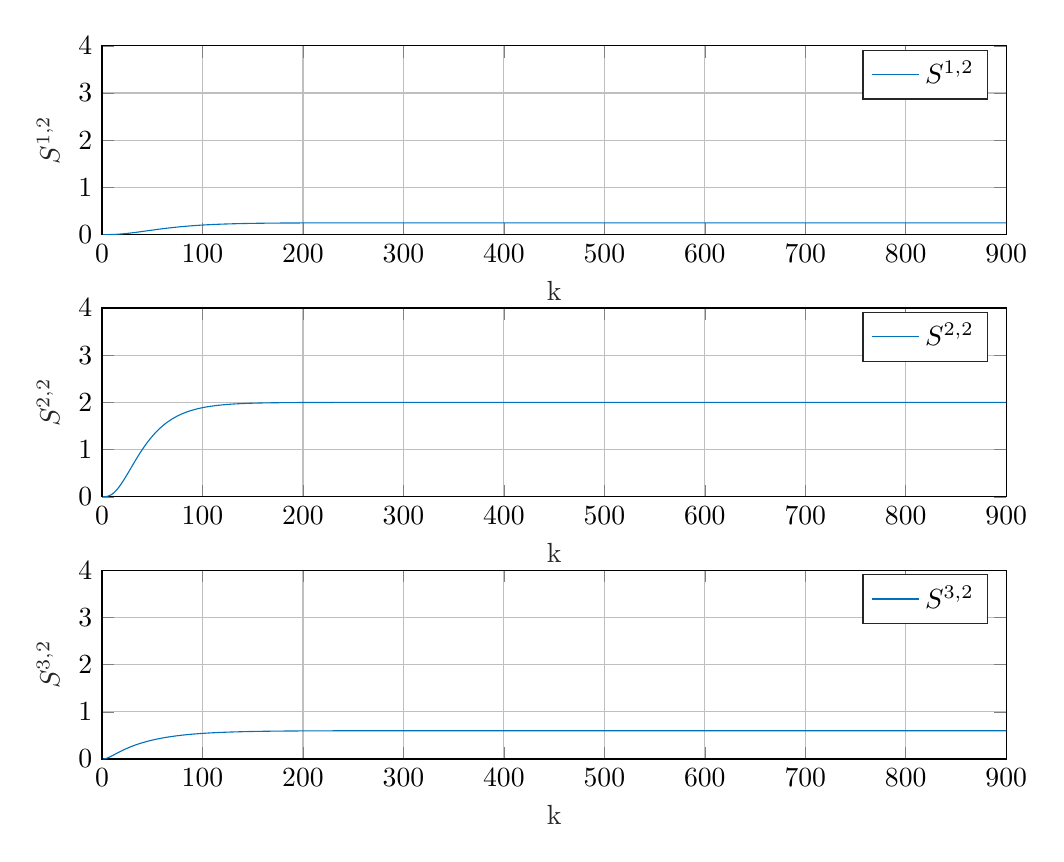
\begin{tikzpicture}

\begin{axis}[%
width=4.521in,
height=0.944in,
at={(0.758in,3.103in)},
scale only axis,
xmin=0,
xmax=900,
xlabel style={font=\color{white!15!black}},
xlabel={k},
ymin=0,
ymax=4,
ylabel style={font=\color{white!15!black}},
ylabel={$\text{S}^{\text{1,2}}$},
axis background/.style={fill=white},
xmajorgrids,
ymajorgrids,
legend style={legend cell align=left, align=left, draw=white!15!black}
]
\addplot [color=mycolor1]
  table[row sep=crcr]{%
1	9.0727e-06\\
2	4.0501e-05\\
3	0.00010895\\
4	0.00022889\\
5	0.00041369\\
6	0.00067524\\
7	0.0010238\\
8	0.0014678\\
9	0.0020142\\
10	0.0026684\\
11	0.0034342\\
12	0.0043145\\
13	0.0053108\\
14	0.0064236\\
15	0.0076526\\
16	0.0089967\\
17	0.010454\\
18	0.012022\\
19	0.013698\\
20	0.015479\\
21	0.01736\\
22	0.019338\\
23	0.021409\\
24	0.023568\\
25	0.025811\\
26	0.028133\\
27	0.030529\\
28	0.032994\\
29	0.035524\\
30	0.038114\\
31	0.040759\\
32	0.043454\\
33	0.046195\\
34	0.048978\\
35	0.051797\\
36	0.054649\\
37	0.05753\\
38	0.060434\\
39	0.06336\\
40	0.066302\\
41	0.069257\\
42	0.072221\\
43	0.075192\\
44	0.078165\\
45	0.081138\\
46	0.084109\\
47	0.087073\\
48	0.090029\\
49	0.092974\\
50	0.095906\\
51	0.098822\\
52	0.10172\\
53	0.1046\\
54	0.10746\\
55	0.11029\\
56	0.1131\\
57	0.11588\\
58	0.11864\\
59	0.12137\\
60	0.12406\\
61	0.12673\\
62	0.12936\\
63	0.13196\\
64	0.13453\\
65	0.13706\\
66	0.13956\\
67	0.14202\\
68	0.14444\\
69	0.14683\\
70	0.14918\\
71	0.15149\\
72	0.15377\\
73	0.15601\\
74	0.15821\\
75	0.16037\\
76	0.16249\\
77	0.16458\\
78	0.16663\\
79	0.16864\\
80	0.17061\\
81	0.17255\\
82	0.17445\\
83	0.17631\\
84	0.17813\\
85	0.17992\\
86	0.18167\\
87	0.18339\\
88	0.18507\\
89	0.18671\\
90	0.18832\\
91	0.1899\\
92	0.19144\\
93	0.19295\\
94	0.19442\\
95	0.19586\\
96	0.19727\\
97	0.19865\\
98	0.2\\
99	0.20132\\
100	0.2026\\
101	0.20386\\
102	0.20509\\
103	0.20628\\
104	0.20745\\
105	0.2086\\
106	0.20971\\
107	0.2108\\
108	0.21186\\
109	0.2129\\
110	0.21391\\
111	0.21489\\
112	0.21585\\
113	0.21679\\
114	0.21771\\
115	0.2186\\
116	0.21947\\
117	0.22031\\
118	0.22114\\
119	0.22194\\
120	0.22272\\
121	0.22349\\
122	0.22423\\
123	0.22495\\
124	0.22566\\
125	0.22635\\
126	0.22702\\
127	0.22767\\
128	0.2283\\
129	0.22892\\
130	0.22952\\
131	0.2301\\
132	0.23067\\
133	0.23123\\
134	0.23176\\
135	0.23229\\
136	0.2328\\
137	0.2333\\
138	0.23378\\
139	0.23425\\
140	0.2347\\
141	0.23515\\
142	0.23558\\
143	0.236\\
144	0.23641\\
145	0.23681\\
146	0.23719\\
147	0.23757\\
148	0.23793\\
149	0.23829\\
150	0.23863\\
151	0.23896\\
152	0.23929\\
153	0.23961\\
154	0.23991\\
155	0.24021\\
156	0.2405\\
157	0.24078\\
158	0.24106\\
159	0.24132\\
160	0.24158\\
161	0.24183\\
162	0.24208\\
163	0.24231\\
164	0.24254\\
165	0.24277\\
166	0.24298\\
167	0.24319\\
168	0.2434\\
169	0.2436\\
170	0.24379\\
171	0.24398\\
172	0.24416\\
173	0.24433\\
174	0.24451\\
175	0.24467\\
176	0.24483\\
177	0.24499\\
178	0.24514\\
179	0.24529\\
180	0.24543\\
181	0.24557\\
182	0.24571\\
183	0.24584\\
184	0.24596\\
185	0.24609\\
186	0.24621\\
187	0.24632\\
188	0.24643\\
189	0.24654\\
190	0.24665\\
191	0.24675\\
192	0.24685\\
193	0.24695\\
194	0.24704\\
195	0.24713\\
196	0.24722\\
197	0.24731\\
198	0.24739\\
199	0.24747\\
200	0.24755\\
201	0.24762\\
202	0.2477\\
203	0.24777\\
204	0.24784\\
205	0.2479\\
206	0.24797\\
207	0.24803\\
208	0.24809\\
209	0.24815\\
210	0.24821\\
211	0.24826\\
212	0.24832\\
213	0.24837\\
214	0.24842\\
215	0.24847\\
216	0.24852\\
217	0.24856\\
218	0.24861\\
219	0.24865\\
220	0.24869\\
221	0.24873\\
222	0.24877\\
223	0.24881\\
224	0.24885\\
225	0.24889\\
226	0.24892\\
227	0.24895\\
228	0.24899\\
229	0.24902\\
230	0.24905\\
231	0.24908\\
232	0.24911\\
233	0.24914\\
234	0.24916\\
235	0.24919\\
236	0.24922\\
237	0.24924\\
238	0.24926\\
239	0.24929\\
240	0.24931\\
241	0.24933\\
242	0.24935\\
243	0.24937\\
244	0.24939\\
245	0.24941\\
246	0.24943\\
247	0.24945\\
248	0.24947\\
249	0.24948\\
250	0.2495\\
251	0.24951\\
252	0.24953\\
253	0.24954\\
254	0.24956\\
255	0.24957\\
256	0.24959\\
257	0.2496\\
258	0.24961\\
259	0.24962\\
260	0.24964\\
261	0.24965\\
262	0.24966\\
263	0.24967\\
264	0.24968\\
265	0.24969\\
266	0.2497\\
267	0.24971\\
268	0.24972\\
269	0.24973\\
270	0.24974\\
271	0.24975\\
272	0.24975\\
273	0.24976\\
274	0.24977\\
275	0.24978\\
276	0.24978\\
277	0.24979\\
278	0.2498\\
279	0.2498\\
280	0.24981\\
281	0.24982\\
282	0.24982\\
283	0.24983\\
284	0.24983\\
285	0.24984\\
286	0.24984\\
287	0.24985\\
288	0.24985\\
289	0.24986\\
290	0.24986\\
291	0.24987\\
292	0.24987\\
293	0.24988\\
294	0.24988\\
295	0.24988\\
296	0.24989\\
297	0.24989\\
298	0.24989\\
299	0.2499\\
300	0.2499\\
301	0.2499\\
302	0.24991\\
303	0.24991\\
304	0.24991\\
305	0.24992\\
306	0.24992\\
307	0.24992\\
308	0.24992\\
309	0.24993\\
310	0.24993\\
311	0.24993\\
312	0.24993\\
313	0.24993\\
314	0.24994\\
315	0.24994\\
316	0.24994\\
317	0.24994\\
318	0.24994\\
319	0.24995\\
320	0.24995\\
321	0.24995\\
322	0.24995\\
323	0.24995\\
324	0.24995\\
325	0.24996\\
326	0.24996\\
327	0.24996\\
328	0.24996\\
329	0.24996\\
330	0.24996\\
331	0.24996\\
332	0.24997\\
333	0.24997\\
334	0.24997\\
335	0.24997\\
336	0.24997\\
337	0.24997\\
338	0.24997\\
339	0.24997\\
340	0.24997\\
341	0.24997\\
342	0.24997\\
343	0.24998\\
344	0.24998\\
345	0.24998\\
346	0.24998\\
347	0.24998\\
348	0.24998\\
349	0.24998\\
350	0.24998\\
351	0.24998\\
352	0.24998\\
353	0.24998\\
354	0.24998\\
355	0.24998\\
356	0.24998\\
357	0.24998\\
358	0.24999\\
359	0.24999\\
360	0.24999\\
361	0.24999\\
362	0.24999\\
363	0.24999\\
364	0.24999\\
365	0.24999\\
366	0.24999\\
367	0.24999\\
368	0.24999\\
369	0.24999\\
370	0.24999\\
371	0.24999\\
372	0.24999\\
373	0.24999\\
374	0.24999\\
375	0.24999\\
376	0.24999\\
377	0.24999\\
378	0.24999\\
379	0.24999\\
380	0.24999\\
381	0.24999\\
382	0.24999\\
383	0.24999\\
384	0.24999\\
385	0.24999\\
386	0.24999\\
387	0.24999\\
388	0.24999\\
389	0.24999\\
390	0.24999\\
391	0.24999\\
392	0.25\\
393	0.25\\
394	0.25\\
395	0.25\\
396	0.25\\
397	0.25\\
398	0.25\\
399	0.25\\
400	0.25\\
401	0.25\\
402	0.25\\
403	0.25\\
404	0.25\\
405	0.25\\
406	0.25\\
407	0.25\\
408	0.25\\
409	0.25\\
410	0.25\\
411	0.25\\
412	0.25\\
413	0.25\\
414	0.25\\
415	0.25\\
416	0.25\\
417	0.25\\
418	0.25\\
419	0.25\\
420	0.25\\
421	0.25\\
422	0.25\\
423	0.25\\
424	0.25\\
425	0.25\\
426	0.25\\
427	0.25\\
428	0.25\\
429	0.25\\
430	0.25\\
431	0.25\\
432	0.25\\
433	0.25\\
434	0.25\\
435	0.25\\
436	0.25\\
437	0.25\\
438	0.25\\
439	0.25\\
440	0.25\\
441	0.25\\
442	0.25\\
443	0.25\\
444	0.25\\
445	0.25\\
446	0.25\\
447	0.25\\
448	0.25\\
449	0.25\\
450	0.25\\
451	0.25\\
452	0.25\\
453	0.25\\
454	0.25\\
455	0.25\\
456	0.25\\
457	0.25\\
458	0.25\\
459	0.25\\
460	0.25\\
461	0.25\\
462	0.25\\
463	0.25\\
464	0.25\\
465	0.25\\
466	0.25\\
467	0.25\\
468	0.25\\
469	0.25\\
470	0.25\\
471	0.25\\
472	0.25\\
473	0.25\\
474	0.25\\
475	0.25\\
476	0.25\\
477	0.25\\
478	0.25\\
479	0.25\\
480	0.25\\
481	0.25\\
482	0.25\\
483	0.25\\
484	0.25\\
485	0.25\\
486	0.25\\
487	0.25\\
488	0.25\\
489	0.25\\
490	0.25\\
491	0.25\\
492	0.25\\
493	0.25\\
494	0.25\\
495	0.25\\
496	0.25\\
497	0.25\\
498	0.25\\
499	0.25\\
500	0.25\\
501	0.25\\
502	0.25\\
503	0.25\\
504	0.25\\
505	0.25\\
506	0.25\\
507	0.25\\
508	0.25\\
509	0.25\\
510	0.25\\
511	0.25\\
512	0.25\\
513	0.25\\
514	0.25\\
515	0.25\\
516	0.25\\
517	0.25\\
518	0.25\\
519	0.25\\
520	0.25\\
521	0.25\\
522	0.25\\
523	0.25\\
524	0.25\\
525	0.25\\
526	0.25\\
527	0.25\\
528	0.25\\
529	0.25\\
530	0.25\\
531	0.25\\
532	0.25\\
533	0.25\\
534	0.25\\
535	0.25\\
536	0.25\\
537	0.25\\
538	0.25\\
539	0.25\\
540	0.25\\
541	0.25\\
542	0.25\\
543	0.25\\
544	0.25\\
545	0.25\\
546	0.25\\
547	0.25\\
548	0.25\\
549	0.25\\
550	0.25\\
551	0.25\\
552	0.25\\
553	0.25\\
554	0.25\\
555	0.25\\
556	0.25\\
557	0.25\\
558	0.25\\
559	0.25\\
560	0.25\\
561	0.25\\
562	0.25\\
563	0.25\\
564	0.25\\
565	0.25\\
566	0.25\\
567	0.25\\
568	0.25\\
569	0.25\\
570	0.25\\
571	0.25\\
572	0.25\\
573	0.25\\
574	0.25\\
575	0.25\\
576	0.25\\
577	0.25\\
578	0.25\\
579	0.25\\
580	0.25\\
581	0.25\\
582	0.25\\
583	0.25\\
584	0.25\\
585	0.25\\
586	0.25\\
587	0.25\\
588	0.25\\
589	0.25\\
590	0.25\\
591	0.25\\
592	0.25\\
593	0.25\\
594	0.25\\
595	0.25\\
596	0.25\\
597	0.25\\
598	0.25\\
599	0.25\\
600	0.25\\
601	0.25\\
602	0.25\\
603	0.25\\
604	0.25\\
605	0.25\\
606	0.25\\
607	0.25\\
608	0.25\\
609	0.25\\
610	0.25\\
611	0.25\\
612	0.25\\
613	0.25\\
614	0.25\\
615	0.25\\
616	0.25\\
617	0.25\\
618	0.25\\
619	0.25\\
620	0.25\\
621	0.25\\
622	0.25\\
623	0.25\\
624	0.25\\
625	0.25\\
626	0.25\\
627	0.25\\
628	0.25\\
629	0.25\\
630	0.25\\
631	0.25\\
632	0.25\\
633	0.25\\
634	0.25\\
635	0.25\\
636	0.25\\
637	0.25\\
638	0.25\\
639	0.25\\
640	0.25\\
641	0.25\\
642	0.25\\
643	0.25\\
644	0.25\\
645	0.25\\
646	0.25\\
647	0.25\\
648	0.25\\
649	0.25\\
650	0.25\\
651	0.25\\
652	0.25\\
653	0.25\\
654	0.25\\
655	0.25\\
656	0.25\\
657	0.25\\
658	0.25\\
659	0.25\\
660	0.25\\
661	0.25\\
662	0.25\\
663	0.25\\
664	0.25\\
665	0.25\\
666	0.25\\
667	0.25\\
668	0.25\\
669	0.25\\
670	0.25\\
671	0.25\\
672	0.25\\
673	0.25\\
674	0.25\\
675	0.25\\
676	0.25\\
677	0.25\\
678	0.25\\
679	0.25\\
680	0.25\\
681	0.25\\
682	0.25\\
683	0.25\\
684	0.25\\
685	0.25\\
686	0.25\\
687	0.25\\
688	0.25\\
689	0.25\\
690	0.25\\
691	0.25\\
692	0.25\\
693	0.25\\
694	0.25\\
695	0.25\\
696	0.25\\
697	0.25\\
698	0.25\\
699	0.25\\
700	0.25\\
701	0.25\\
702	0.25\\
703	0.25\\
704	0.25\\
705	0.25\\
706	0.25\\
707	0.25\\
708	0.25\\
709	0.25\\
710	0.25\\
711	0.25\\
712	0.25\\
713	0.25\\
714	0.25\\
715	0.25\\
716	0.25\\
717	0.25\\
718	0.25\\
719	0.25\\
720	0.25\\
721	0.25\\
722	0.25\\
723	0.25\\
724	0.25\\
725	0.25\\
726	0.25\\
727	0.25\\
728	0.25\\
729	0.25\\
730	0.25\\
731	0.25\\
732	0.25\\
733	0.25\\
734	0.25\\
735	0.25\\
736	0.25\\
737	0.25\\
738	0.25\\
739	0.25\\
740	0.25\\
741	0.25\\
742	0.25\\
743	0.25\\
744	0.25\\
745	0.25\\
746	0.25\\
747	0.25\\
748	0.25\\
749	0.25\\
750	0.25\\
751	0.25\\
752	0.25\\
753	0.25\\
754	0.25\\
755	0.25\\
756	0.25\\
757	0.25\\
758	0.25\\
759	0.25\\
760	0.25\\
761	0.25\\
762	0.25\\
763	0.25\\
764	0.25\\
765	0.25\\
766	0.25\\
767	0.25\\
768	0.25\\
769	0.25\\
770	0.25\\
771	0.25\\
772	0.25\\
773	0.25\\
774	0.25\\
775	0.25\\
776	0.25\\
777	0.25\\
778	0.25\\
779	0.25\\
780	0.25\\
781	0.25\\
782	0.25\\
783	0.25\\
784	0.25\\
785	0.25\\
786	0.25\\
787	0.25\\
788	0.25\\
789	0.25\\
790	0.25\\
791	0.25\\
792	0.25\\
793	0.25\\
794	0.25\\
795	0.25\\
796	0.25\\
797	0.25\\
798	0.25\\
799	0.25\\
800	0.25\\
801	0.25\\
802	0.25\\
803	0.25\\
804	0.25\\
805	0.25\\
806	0.25\\
807	0.25\\
808	0.25\\
809	0.25\\
810	0.25\\
811	0.25\\
812	0.25\\
813	0.25\\
814	0.25\\
815	0.25\\
816	0.25\\
817	0.25\\
818	0.25\\
819	0.25\\
820	0.25\\
821	0.25\\
822	0.25\\
823	0.25\\
824	0.25\\
825	0.25\\
826	0.25\\
827	0.25\\
828	0.25\\
829	0.25\\
830	0.25\\
831	0.25\\
832	0.25\\
833	0.25\\
834	0.25\\
835	0.25\\
836	0.25\\
837	0.25\\
838	0.25\\
839	0.25\\
840	0.25\\
841	0.25\\
842	0.25\\
843	0.25\\
844	0.25\\
845	0.25\\
846	0.25\\
847	0.25\\
848	0.25\\
849	0.25\\
850	0.25\\
851	0.25\\
852	0.25\\
853	0.25\\
854	0.25\\
855	0.25\\
856	0.25\\
857	0.25\\
858	0.25\\
859	0.25\\
860	0.25\\
861	0.25\\
862	0.25\\
863	0.25\\
864	0.25\\
865	0.25\\
866	0.25\\
867	0.25\\
868	0.25\\
869	0.25\\
870	0.25\\
871	0.25\\
872	0.25\\
873	0.25\\
874	0.25\\
875	0.25\\
876	0.25\\
877	0.25\\
878	0.25\\
879	0.25\\
880	0.25\\
881	0.25\\
882	0.25\\
883	0.25\\
884	0.25\\
885	0.25\\
886	0.25\\
887	0.25\\
888	0.25\\
889	0.25\\
890	0.25\\
891	0.25\\
892	0.25\\
893	0.25\\
894	0.25\\
895	0.25\\
896	0.25\\
897	0.25\\
898	0.25\\
899	0.25\\
900	0.25\\
};
\addlegendentry{$\text{S}^{\text{1,2}}$}

\end{axis}

\begin{axis}[%
width=4.521in,
height=0.944in,
at={(0.758in,1.792in)},
scale only axis,
xmin=0,
xmax=900,
xlabel style={font=\color{white!15!black}},
xlabel={k},
ymin=0,
ymax=4,
ylabel style={font=\color{white!15!black}},
ylabel={$\text{S}^{\text{2,2}}$},
axis background/.style={fill=white},
xmajorgrids,
ymajorgrids,
legend style={legend cell align=left, align=left, draw=white!15!black}
]
\addplot [color=mycolor1]
  table[row sep=crcr]{%
1	0.00018665\\
2	0.00084523\\
3	0.0022992\\
4	0.0048701\\
5	0.008852\\
6	0.014497\\
7	0.022007\\
8	0.031532\\
9	0.043173\\
10	0.056982\\
11	0.072969\\
12	0.091108\\
13	0.11134\\
14	0.13358\\
15	0.15772\\
16	0.18364\\
17	0.2112\\
18	0.24027\\
19	0.2707\\
20	0.30234\\
21	0.33503\\
22	0.36864\\
23	0.40302\\
24	0.43802\\
25	0.47353\\
26	0.50942\\
27	0.54556\\
28	0.58184\\
29	0.61817\\
30	0.65446\\
31	0.6906\\
32	0.72652\\
33	0.76216\\
34	0.79744\\
35	0.83231\\
36	0.86671\\
37	0.9006\\
38	0.93394\\
39	0.9667\\
40	0.99884\\
41	1.0303\\
42	1.0612\\
43	1.0913\\
44	1.1208\\
45	1.1496\\
46	1.1776\\
47	1.205\\
48	1.2316\\
49	1.2575\\
50	1.2827\\
51	1.3072\\
52	1.331\\
53	1.3541\\
54	1.3765\\
55	1.3983\\
56	1.4193\\
57	1.4398\\
58	1.4596\\
59	1.4787\\
60	1.4973\\
61	1.5152\\
62	1.5326\\
63	1.5494\\
64	1.5656\\
65	1.5813\\
66	1.5965\\
67	1.6111\\
68	1.6253\\
69	1.6389\\
70	1.6521\\
71	1.6648\\
72	1.6771\\
73	1.689\\
74	1.7004\\
75	1.7115\\
76	1.7221\\
77	1.7324\\
78	1.7423\\
79	1.7518\\
80	1.761\\
81	1.7699\\
82	1.7784\\
83	1.7866\\
84	1.7946\\
85	1.8022\\
86	1.8096\\
87	1.8167\\
88	1.8235\\
89	1.8301\\
90	1.8365\\
91	1.8426\\
92	1.8485\\
93	1.8541\\
94	1.8596\\
95	1.8649\\
96	1.8699\\
97	1.8748\\
98	1.8795\\
99	1.884\\
100	1.8884\\
101	1.8926\\
102	1.8966\\
103	1.9005\\
104	1.9042\\
105	1.9078\\
106	1.9113\\
107	1.9146\\
108	1.9178\\
109	1.9209\\
110	1.9239\\
111	1.9268\\
112	1.9295\\
113	1.9322\\
114	1.9347\\
115	1.9372\\
116	1.9395\\
117	1.9418\\
118	1.944\\
119	1.9461\\
120	1.9481\\
121	1.9501\\
122	1.952\\
123	1.9538\\
124	1.9555\\
125	1.9572\\
126	1.9588\\
127	1.9604\\
128	1.9619\\
129	1.9633\\
130	1.9647\\
131	1.966\\
132	1.9673\\
133	1.9685\\
134	1.9697\\
135	1.9709\\
136	1.972\\
137	1.973\\
138	1.974\\
139	1.975\\
140	1.976\\
141	1.9769\\
142	1.9777\\
143	1.9786\\
144	1.9794\\
145	1.9802\\
146	1.9809\\
147	1.9816\\
148	1.9823\\
149	1.983\\
150	1.9836\\
151	1.9842\\
152	1.9848\\
153	1.9854\\
154	1.986\\
155	1.9865\\
156	1.987\\
157	1.9875\\
158	1.988\\
159	1.9884\\
160	1.9889\\
161	1.9893\\
162	1.9897\\
163	1.9901\\
164	1.9904\\
165	1.9908\\
166	1.9912\\
167	1.9915\\
168	1.9918\\
169	1.9921\\
170	1.9924\\
171	1.9927\\
172	1.993\\
173	1.9932\\
174	1.9935\\
175	1.9937\\
176	1.994\\
177	1.9942\\
178	1.9944\\
179	1.9946\\
180	1.9948\\
181	1.995\\
182	1.9952\\
183	1.9954\\
184	1.9956\\
185	1.9957\\
186	1.9959\\
187	1.9961\\
188	1.9962\\
189	1.9963\\
190	1.9965\\
191	1.9966\\
192	1.9967\\
193	1.9969\\
194	1.997\\
195	1.9971\\
196	1.9972\\
197	1.9973\\
198	1.9974\\
199	1.9975\\
200	1.9976\\
201	1.9977\\
202	1.9978\\
203	1.9979\\
204	1.9979\\
205	1.998\\
206	1.9981\\
207	1.9982\\
208	1.9982\\
209	1.9983\\
210	1.9984\\
211	1.9984\\
212	1.9985\\
213	1.9985\\
214	1.9986\\
215	1.9987\\
216	1.9987\\
217	1.9988\\
218	1.9988\\
219	1.9988\\
220	1.9989\\
221	1.9989\\
222	1.999\\
223	1.999\\
224	1.999\\
225	1.9991\\
226	1.9991\\
227	1.9992\\
228	1.9992\\
229	1.9992\\
230	1.9992\\
231	1.9993\\
232	1.9993\\
233	1.9993\\
234	1.9994\\
235	1.9994\\
236	1.9994\\
237	1.9994\\
238	1.9994\\
239	1.9995\\
240	1.9995\\
241	1.9995\\
242	1.9995\\
243	1.9995\\
244	1.9996\\
245	1.9996\\
246	1.9996\\
247	1.9996\\
248	1.9996\\
249	1.9996\\
250	1.9997\\
251	1.9997\\
252	1.9997\\
253	1.9997\\
254	1.9997\\
255	1.9997\\
256	1.9997\\
257	1.9997\\
258	1.9997\\
259	1.9998\\
260	1.9998\\
261	1.9998\\
262	1.9998\\
263	1.9998\\
264	1.9998\\
265	1.9998\\
266	1.9998\\
267	1.9998\\
268	1.9998\\
269	1.9998\\
270	1.9998\\
271	1.9998\\
272	1.9998\\
273	1.9999\\
274	1.9999\\
275	1.9999\\
276	1.9999\\
277	1.9999\\
278	1.9999\\
279	1.9999\\
280	1.9999\\
281	1.9999\\
282	1.9999\\
283	1.9999\\
284	1.9999\\
285	1.9999\\
286	1.9999\\
287	1.9999\\
288	1.9999\\
289	1.9999\\
290	1.9999\\
291	1.9999\\
292	1.9999\\
293	1.9999\\
294	1.9999\\
295	1.9999\\
296	1.9999\\
297	1.9999\\
298	1.9999\\
299	1.9999\\
300	1.9999\\
301	2\\
302	2\\
303	2\\
304	2\\
305	2\\
306	2\\
307	2\\
308	2\\
309	2\\
310	2\\
311	2\\
312	2\\
313	2\\
314	2\\
315	2\\
316	2\\
317	2\\
318	2\\
319	2\\
320	2\\
321	2\\
322	2\\
323	2\\
324	2\\
325	2\\
326	2\\
327	2\\
328	2\\
329	2\\
330	2\\
331	2\\
332	2\\
333	2\\
334	2\\
335	2\\
336	2\\
337	2\\
338	2\\
339	2\\
340	2\\
341	2\\
342	2\\
343	2\\
344	2\\
345	2\\
346	2\\
347	2\\
348	2\\
349	2\\
350	2\\
351	2\\
352	2\\
353	2\\
354	2\\
355	2\\
356	2\\
357	2\\
358	2\\
359	2\\
360	2\\
361	2\\
362	2\\
363	2\\
364	2\\
365	2\\
366	2\\
367	2\\
368	2\\
369	2\\
370	2\\
371	2\\
372	2\\
373	2\\
374	2\\
375	2\\
376	2\\
377	2\\
378	2\\
379	2\\
380	2\\
381	2\\
382	2\\
383	2\\
384	2\\
385	2\\
386	2\\
387	2\\
388	2\\
389	2\\
390	2\\
391	2\\
392	2\\
393	2\\
394	2\\
395	2\\
396	2\\
397	2\\
398	2\\
399	2\\
400	2\\
401	2\\
402	2\\
403	2\\
404	2\\
405	2\\
406	2\\
407	2\\
408	2\\
409	2\\
410	2\\
411	2\\
412	2\\
413	2\\
414	2\\
415	2\\
416	2\\
417	2\\
418	2\\
419	2\\
420	2\\
421	2\\
422	2\\
423	2\\
424	2\\
425	2\\
426	2\\
427	2\\
428	2\\
429	2\\
430	2\\
431	2\\
432	2\\
433	2\\
434	2\\
435	2\\
436	2\\
437	2\\
438	2\\
439	2\\
440	2\\
441	2\\
442	2\\
443	2\\
444	2\\
445	2\\
446	2\\
447	2\\
448	2\\
449	2\\
450	2\\
451	2\\
452	2\\
453	2\\
454	2\\
455	2\\
456	2\\
457	2\\
458	2\\
459	2\\
460	2\\
461	2\\
462	2\\
463	2\\
464	2\\
465	2\\
466	2\\
467	2\\
468	2\\
469	2\\
470	2\\
471	2\\
472	2\\
473	2\\
474	2\\
475	2\\
476	2\\
477	2\\
478	2\\
479	2\\
480	2\\
481	2\\
482	2\\
483	2\\
484	2\\
485	2\\
486	2\\
487	2\\
488	2\\
489	2\\
490	2\\
491	2\\
492	2\\
493	2\\
494	2\\
495	2\\
496	2\\
497	2\\
498	2\\
499	2\\
500	2\\
501	2\\
502	2\\
503	2\\
504	2\\
505	2\\
506	2\\
507	2\\
508	2\\
509	2\\
510	2\\
511	2\\
512	2\\
513	2\\
514	2\\
515	2\\
516	2\\
517	2\\
518	2\\
519	2\\
520	2\\
521	2\\
522	2\\
523	2\\
524	2\\
525	2\\
526	2\\
527	2\\
528	2\\
529	2\\
530	2\\
531	2\\
532	2\\
533	2\\
534	2\\
535	2\\
536	2\\
537	2\\
538	2\\
539	2\\
540	2\\
541	2\\
542	2\\
543	2\\
544	2\\
545	2\\
546	2\\
547	2\\
548	2\\
549	2\\
550	2\\
551	2\\
552	2\\
553	2\\
554	2\\
555	2\\
556	2\\
557	2\\
558	2\\
559	2\\
560	2\\
561	2\\
562	2\\
563	2\\
564	2\\
565	2\\
566	2\\
567	2\\
568	2\\
569	2\\
570	2\\
571	2\\
572	2\\
573	2\\
574	2\\
575	2\\
576	2\\
577	2\\
578	2\\
579	2\\
580	2\\
581	2\\
582	2\\
583	2\\
584	2\\
585	2\\
586	2\\
587	2\\
588	2\\
589	2\\
590	2\\
591	2\\
592	2\\
593	2\\
594	2\\
595	2\\
596	2\\
597	2\\
598	2\\
599	2\\
600	2\\
601	2\\
602	2\\
603	2\\
604	2\\
605	2\\
606	2\\
607	2\\
608	2\\
609	2\\
610	2\\
611	2\\
612	2\\
613	2\\
614	2\\
615	2\\
616	2\\
617	2\\
618	2\\
619	2\\
620	2\\
621	2\\
622	2\\
623	2\\
624	2\\
625	2\\
626	2\\
627	2\\
628	2\\
629	2\\
630	2\\
631	2\\
632	2\\
633	2\\
634	2\\
635	2\\
636	2\\
637	2\\
638	2\\
639	2\\
640	2\\
641	2\\
642	2\\
643	2\\
644	2\\
645	2\\
646	2\\
647	2\\
648	2\\
649	2\\
650	2\\
651	2\\
652	2\\
653	2\\
654	2\\
655	2\\
656	2\\
657	2\\
658	2\\
659	2\\
660	2\\
661	2\\
662	2\\
663	2\\
664	2\\
665	2\\
666	2\\
667	2\\
668	2\\
669	2\\
670	2\\
671	2\\
672	2\\
673	2\\
674	2\\
675	2\\
676	2\\
677	2\\
678	2\\
679	2\\
680	2\\
681	2\\
682	2\\
683	2\\
684	2\\
685	2\\
686	2\\
687	2\\
688	2\\
689	2\\
690	2\\
691	2\\
692	2\\
693	2\\
694	2\\
695	2\\
696	2\\
697	2\\
698	2\\
699	2\\
700	2\\
701	2\\
702	2\\
703	2\\
704	2\\
705	2\\
706	2\\
707	2\\
708	2\\
709	2\\
710	2\\
711	2\\
712	2\\
713	2\\
714	2\\
715	2\\
716	2\\
717	2\\
718	2\\
719	2\\
720	2\\
721	2\\
722	2\\
723	2\\
724	2\\
725	2\\
726	2\\
727	2\\
728	2\\
729	2\\
730	2\\
731	2\\
732	2\\
733	2\\
734	2\\
735	2\\
736	2\\
737	2\\
738	2\\
739	2\\
740	2\\
741	2\\
742	2\\
743	2\\
744	2\\
745	2\\
746	2\\
747	2\\
748	2\\
749	2\\
750	2\\
751	2\\
752	2\\
753	2\\
754	2\\
755	2\\
756	2\\
757	2\\
758	2\\
759	2\\
760	2\\
761	2\\
762	2\\
763	2\\
764	2\\
765	2\\
766	2\\
767	2\\
768	2\\
769	2\\
770	2\\
771	2\\
772	2\\
773	2\\
774	2\\
775	2\\
776	2\\
777	2\\
778	2\\
779	2\\
780	2\\
781	2\\
782	2\\
783	2\\
784	2\\
785	2\\
786	2\\
787	2\\
788	2\\
789	2\\
790	2\\
791	2\\
792	2\\
793	2\\
794	2\\
795	2\\
796	2\\
797	2\\
798	2\\
799	2\\
800	2\\
801	2\\
802	2\\
803	2\\
804	2\\
805	2\\
806	2\\
807	2\\
808	2\\
809	2\\
810	2\\
811	2\\
812	2\\
813	2\\
814	2\\
815	2\\
816	2\\
817	2\\
818	2\\
819	2\\
820	2\\
821	2\\
822	2\\
823	2\\
824	2\\
825	2\\
826	2\\
827	2\\
828	2\\
829	2\\
830	2\\
831	2\\
832	2\\
833	2\\
834	2\\
835	2\\
836	2\\
837	2\\
838	2\\
839	2\\
840	2\\
841	2\\
842	2\\
843	2\\
844	2\\
845	2\\
846	2\\
847	2\\
848	2\\
849	2\\
850	2\\
851	2\\
852	2\\
853	2\\
854	2\\
855	2\\
856	2\\
857	2\\
858	2\\
859	2\\
860	2\\
861	2\\
862	2\\
863	2\\
864	2\\
865	2\\
866	2\\
867	2\\
868	2\\
869	2\\
870	2\\
871	2\\
872	2\\
873	2\\
874	2\\
875	2\\
876	2\\
877	2\\
878	2\\
879	2\\
880	2\\
881	2\\
882	2\\
883	2\\
884	2\\
885	2\\
886	2\\
887	2\\
888	2\\
889	2\\
890	2\\
891	2\\
892	2\\
893	2\\
894	2\\
895	2\\
896	2\\
897	2\\
898	2\\
899	2\\
900	2\\
};
\addlegendentry{$\text{S}^{\text{2,2}}$}

\end{axis}

\begin{axis}[%
width=4.521in,
height=0.944in,
at={(0.758in,0.481in)},
scale only axis,
xmin=0,
xmax=900,
xlabel style={font=\color{white!15!black}},
xlabel={k},
ymin=0,
ymax=4,
ylabel style={font=\color{white!15!black}},
ylabel={$\text{S}^{\text{3,2}}$},
axis background/.style={fill=white},
xmajorgrids,
ymajorgrids,
legend style={legend cell align=left, align=left, draw=white!15!black}
]
\addplot [color=mycolor1]
  table[row sep=crcr]{%
1	0.00081502\\
2	0.0030388\\
3	0.0069125\\
4	0.012418\\
5	0.01939\\
6	0.0276\\
7	0.036804\\
8	0.046776\\
9	0.057313\\
10	0.068246\\
11	0.079432\\
12	0.09076\\
13	0.10214\\
14	0.11349\\
15	0.12477\\
16	0.13593\\
17	0.14694\\
18	0.15778\\
19	0.16843\\
20	0.17887\\
21	0.18911\\
22	0.19912\\
23	0.20892\\
24	0.2185\\
25	0.22786\\
26	0.237\\
27	0.24592\\
28	0.25464\\
29	0.26314\\
30	0.27144\\
31	0.27954\\
32	0.28744\\
33	0.29515\\
34	0.30267\\
35	0.31001\\
36	0.31716\\
37	0.32414\\
38	0.33095\\
39	0.33759\\
40	0.34407\\
41	0.35039\\
42	0.35655\\
43	0.36256\\
44	0.36842\\
45	0.37414\\
46	0.37971\\
47	0.38515\\
48	0.39046\\
49	0.39563\\
50	0.40068\\
51	0.4056\\
52	0.4104\\
53	0.41508\\
54	0.41964\\
55	0.4241\\
56	0.42844\\
57	0.43268\\
58	0.43681\\
59	0.44084\\
60	0.44477\\
61	0.4486\\
62	0.45234\\
63	0.45598\\
64	0.45954\\
65	0.46301\\
66	0.46639\\
67	0.46969\\
68	0.47291\\
69	0.47604\\
70	0.4791\\
71	0.48209\\
72	0.485\\
73	0.48784\\
74	0.49061\\
75	0.49331\\
76	0.49594\\
77	0.49851\\
78	0.50102\\
79	0.50346\\
80	0.50585\\
81	0.50817\\
82	0.51044\\
83	0.51265\\
84	0.51481\\
85	0.51691\\
86	0.51896\\
87	0.52096\\
88	0.52291\\
89	0.52482\\
90	0.52667\\
91	0.52848\\
92	0.53025\\
93	0.53197\\
94	0.53365\\
95	0.53529\\
96	0.53689\\
97	0.53844\\
98	0.53996\\
99	0.54145\\
100	0.54289\\
101	0.5443\\
102	0.54568\\
103	0.54702\\
104	0.54833\\
105	0.5496\\
106	0.55085\\
107	0.55206\\
108	0.55324\\
109	0.5544\\
110	0.55552\\
111	0.55662\\
112	0.55769\\
113	0.55874\\
114	0.55976\\
115	0.56075\\
116	0.56172\\
117	0.56266\\
118	0.56359\\
119	0.56449\\
120	0.56536\\
121	0.56622\\
122	0.56705\\
123	0.56787\\
124	0.56866\\
125	0.56943\\
126	0.57019\\
127	0.57092\\
128	0.57164\\
129	0.57234\\
130	0.57302\\
131	0.57369\\
132	0.57434\\
133	0.57497\\
134	0.57559\\
135	0.57619\\
136	0.57678\\
137	0.57736\\
138	0.57791\\
139	0.57846\\
140	0.57899\\
141	0.57951\\
142	0.58002\\
143	0.58051\\
144	0.58099\\
145	0.58146\\
146	0.58192\\
147	0.58236\\
148	0.5828\\
149	0.58322\\
150	0.58364\\
151	0.58404\\
152	0.58444\\
153	0.58482\\
154	0.5852\\
155	0.58556\\
156	0.58592\\
157	0.58627\\
158	0.5866\\
159	0.58694\\
160	0.58726\\
161	0.58757\\
162	0.58788\\
163	0.58818\\
164	0.58847\\
165	0.58875\\
166	0.58903\\
167	0.5893\\
168	0.58957\\
169	0.58983\\
170	0.59008\\
171	0.59032\\
172	0.59056\\
173	0.59079\\
174	0.59102\\
175	0.59124\\
176	0.59146\\
177	0.59167\\
178	0.59188\\
179	0.59208\\
180	0.59227\\
181	0.59246\\
182	0.59265\\
183	0.59283\\
184	0.59301\\
185	0.59318\\
186	0.59335\\
187	0.59351\\
188	0.59367\\
189	0.59383\\
190	0.59398\\
191	0.59413\\
192	0.59427\\
193	0.59442\\
194	0.59455\\
195	0.59469\\
196	0.59482\\
197	0.59495\\
198	0.59507\\
199	0.59519\\
200	0.59531\\
201	0.59543\\
202	0.59554\\
203	0.59565\\
204	0.59576\\
205	0.59586\\
206	0.59597\\
207	0.59606\\
208	0.59616\\
209	0.59626\\
210	0.59635\\
211	0.59644\\
212	0.59653\\
213	0.59661\\
214	0.5967\\
215	0.59678\\
216	0.59686\\
217	0.59694\\
218	0.59701\\
219	0.59708\\
220	0.59716\\
221	0.59723\\
222	0.5973\\
223	0.59736\\
224	0.59743\\
225	0.59749\\
226	0.59755\\
227	0.59761\\
228	0.59767\\
229	0.59773\\
230	0.59779\\
231	0.59784\\
232	0.59789\\
233	0.59795\\
234	0.598\\
235	0.59805\\
236	0.59809\\
237	0.59814\\
238	0.59819\\
239	0.59823\\
240	0.59828\\
241	0.59832\\
242	0.59836\\
243	0.5984\\
244	0.59844\\
245	0.59848\\
246	0.59852\\
247	0.59855\\
248	0.59859\\
249	0.59862\\
250	0.59866\\
251	0.59869\\
252	0.59872\\
253	0.59875\\
254	0.59878\\
255	0.59881\\
256	0.59884\\
257	0.59887\\
258	0.5989\\
259	0.59893\\
260	0.59895\\
261	0.59898\\
262	0.59901\\
263	0.59903\\
264	0.59905\\
265	0.59908\\
266	0.5991\\
267	0.59912\\
268	0.59914\\
269	0.59916\\
270	0.59919\\
271	0.59921\\
272	0.59923\\
273	0.59924\\
274	0.59926\\
275	0.59928\\
276	0.5993\\
277	0.59932\\
278	0.59933\\
279	0.59935\\
280	0.59937\\
281	0.59938\\
282	0.5994\\
283	0.59941\\
284	0.59943\\
285	0.59944\\
286	0.59945\\
287	0.59947\\
288	0.59948\\
289	0.59949\\
290	0.59951\\
291	0.59952\\
292	0.59953\\
293	0.59954\\
294	0.59955\\
295	0.59956\\
296	0.59957\\
297	0.59959\\
298	0.5996\\
299	0.59961\\
300	0.59962\\
301	0.59962\\
302	0.59963\\
303	0.59964\\
304	0.59965\\
305	0.59966\\
306	0.59967\\
307	0.59968\\
308	0.59968\\
309	0.59969\\
310	0.5997\\
311	0.59971\\
312	0.59971\\
313	0.59972\\
314	0.59973\\
315	0.59974\\
316	0.59974\\
317	0.59975\\
318	0.59975\\
319	0.59976\\
320	0.59977\\
321	0.59977\\
322	0.59978\\
323	0.59978\\
324	0.59979\\
325	0.59979\\
326	0.5998\\
327	0.5998\\
328	0.59981\\
329	0.59981\\
330	0.59982\\
331	0.59982\\
332	0.59983\\
333	0.59983\\
334	0.59984\\
335	0.59984\\
336	0.59984\\
337	0.59985\\
338	0.59985\\
339	0.59985\\
340	0.59986\\
341	0.59986\\
342	0.59987\\
343	0.59987\\
344	0.59987\\
345	0.59988\\
346	0.59988\\
347	0.59988\\
348	0.59988\\
349	0.59989\\
350	0.59989\\
351	0.59989\\
352	0.5999\\
353	0.5999\\
354	0.5999\\
355	0.5999\\
356	0.59991\\
357	0.59991\\
358	0.59991\\
359	0.59991\\
360	0.59991\\
361	0.59992\\
362	0.59992\\
363	0.59992\\
364	0.59992\\
365	0.59992\\
366	0.59993\\
367	0.59993\\
368	0.59993\\
369	0.59993\\
370	0.59993\\
371	0.59993\\
372	0.59994\\
373	0.59994\\
374	0.59994\\
375	0.59994\\
376	0.59994\\
377	0.59994\\
378	0.59995\\
379	0.59995\\
380	0.59995\\
381	0.59995\\
382	0.59995\\
383	0.59995\\
384	0.59995\\
385	0.59995\\
386	0.59996\\
387	0.59996\\
388	0.59996\\
389	0.59996\\
390	0.59996\\
391	0.59996\\
392	0.59996\\
393	0.59996\\
394	0.59996\\
395	0.59996\\
396	0.59997\\
397	0.59997\\
398	0.59997\\
399	0.59997\\
400	0.59997\\
401	0.59997\\
402	0.59997\\
403	0.59997\\
404	0.59997\\
405	0.59997\\
406	0.59997\\
407	0.59997\\
408	0.59997\\
409	0.59997\\
410	0.59998\\
411	0.59998\\
412	0.59998\\
413	0.59998\\
414	0.59998\\
415	0.59998\\
416	0.59998\\
417	0.59998\\
418	0.59998\\
419	0.59998\\
420	0.59998\\
421	0.59998\\
422	0.59998\\
423	0.59998\\
424	0.59998\\
425	0.59998\\
426	0.59998\\
427	0.59998\\
428	0.59998\\
429	0.59998\\
430	0.59999\\
431	0.59999\\
432	0.59999\\
433	0.59999\\
434	0.59999\\
435	0.59999\\
436	0.59999\\
437	0.59999\\
438	0.59999\\
439	0.59999\\
440	0.59999\\
441	0.59999\\
442	0.59999\\
443	0.59999\\
444	0.59999\\
445	0.59999\\
446	0.59999\\
447	0.59999\\
448	0.59999\\
449	0.59999\\
450	0.59999\\
451	0.59999\\
452	0.59999\\
453	0.59999\\
454	0.59999\\
455	0.59999\\
456	0.59999\\
457	0.59999\\
458	0.59999\\
459	0.59999\\
460	0.59999\\
461	0.59999\\
462	0.59999\\
463	0.59999\\
464	0.59999\\
465	0.59999\\
466	0.59999\\
467	0.59999\\
468	0.59999\\
469	0.59999\\
470	0.59999\\
471	0.59999\\
472	0.59999\\
473	0.59999\\
474	0.6\\
475	0.6\\
476	0.6\\
477	0.6\\
478	0.6\\
479	0.6\\
480	0.6\\
481	0.6\\
482	0.6\\
483	0.6\\
484	0.6\\
485	0.6\\
486	0.6\\
487	0.6\\
488	0.6\\
489	0.6\\
490	0.6\\
491	0.6\\
492	0.6\\
493	0.6\\
494	0.6\\
495	0.6\\
496	0.6\\
497	0.6\\
498	0.6\\
499	0.6\\
500	0.6\\
501	0.6\\
502	0.6\\
503	0.6\\
504	0.6\\
505	0.6\\
506	0.6\\
507	0.6\\
508	0.6\\
509	0.6\\
510	0.6\\
511	0.6\\
512	0.6\\
513	0.6\\
514	0.6\\
515	0.6\\
516	0.6\\
517	0.6\\
518	0.6\\
519	0.6\\
520	0.6\\
521	0.6\\
522	0.6\\
523	0.6\\
524	0.6\\
525	0.6\\
526	0.6\\
527	0.6\\
528	0.6\\
529	0.6\\
530	0.6\\
531	0.6\\
532	0.6\\
533	0.6\\
534	0.6\\
535	0.6\\
536	0.6\\
537	0.6\\
538	0.6\\
539	0.6\\
540	0.6\\
541	0.6\\
542	0.6\\
543	0.6\\
544	0.6\\
545	0.6\\
546	0.6\\
547	0.6\\
548	0.6\\
549	0.6\\
550	0.6\\
551	0.6\\
552	0.6\\
553	0.6\\
554	0.6\\
555	0.6\\
556	0.6\\
557	0.6\\
558	0.6\\
559	0.6\\
560	0.6\\
561	0.6\\
562	0.6\\
563	0.6\\
564	0.6\\
565	0.6\\
566	0.6\\
567	0.6\\
568	0.6\\
569	0.6\\
570	0.6\\
571	0.6\\
572	0.6\\
573	0.6\\
574	0.6\\
575	0.6\\
576	0.6\\
577	0.6\\
578	0.6\\
579	0.6\\
580	0.6\\
581	0.6\\
582	0.6\\
583	0.6\\
584	0.6\\
585	0.6\\
586	0.6\\
587	0.6\\
588	0.6\\
589	0.6\\
590	0.6\\
591	0.6\\
592	0.6\\
593	0.6\\
594	0.6\\
595	0.6\\
596	0.6\\
597	0.6\\
598	0.6\\
599	0.6\\
600	0.6\\
601	0.6\\
602	0.6\\
603	0.6\\
604	0.6\\
605	0.6\\
606	0.6\\
607	0.6\\
608	0.6\\
609	0.6\\
610	0.6\\
611	0.6\\
612	0.6\\
613	0.6\\
614	0.6\\
615	0.6\\
616	0.6\\
617	0.6\\
618	0.6\\
619	0.6\\
620	0.6\\
621	0.6\\
622	0.6\\
623	0.6\\
624	0.6\\
625	0.6\\
626	0.6\\
627	0.6\\
628	0.6\\
629	0.6\\
630	0.6\\
631	0.6\\
632	0.6\\
633	0.6\\
634	0.6\\
635	0.6\\
636	0.6\\
637	0.6\\
638	0.6\\
639	0.6\\
640	0.6\\
641	0.6\\
642	0.6\\
643	0.6\\
644	0.6\\
645	0.6\\
646	0.6\\
647	0.6\\
648	0.6\\
649	0.6\\
650	0.6\\
651	0.6\\
652	0.6\\
653	0.6\\
654	0.6\\
655	0.6\\
656	0.6\\
657	0.6\\
658	0.6\\
659	0.6\\
660	0.6\\
661	0.6\\
662	0.6\\
663	0.6\\
664	0.6\\
665	0.6\\
666	0.6\\
667	0.6\\
668	0.6\\
669	0.6\\
670	0.6\\
671	0.6\\
672	0.6\\
673	0.6\\
674	0.6\\
675	0.6\\
676	0.6\\
677	0.6\\
678	0.6\\
679	0.6\\
680	0.6\\
681	0.6\\
682	0.6\\
683	0.6\\
684	0.6\\
685	0.6\\
686	0.6\\
687	0.6\\
688	0.6\\
689	0.6\\
690	0.6\\
691	0.6\\
692	0.6\\
693	0.6\\
694	0.6\\
695	0.6\\
696	0.6\\
697	0.6\\
698	0.6\\
699	0.6\\
700	0.6\\
701	0.6\\
702	0.6\\
703	0.6\\
704	0.6\\
705	0.6\\
706	0.6\\
707	0.6\\
708	0.6\\
709	0.6\\
710	0.6\\
711	0.6\\
712	0.6\\
713	0.6\\
714	0.6\\
715	0.6\\
716	0.6\\
717	0.6\\
718	0.6\\
719	0.6\\
720	0.6\\
721	0.6\\
722	0.6\\
723	0.6\\
724	0.6\\
725	0.6\\
726	0.6\\
727	0.6\\
728	0.6\\
729	0.6\\
730	0.6\\
731	0.6\\
732	0.6\\
733	0.6\\
734	0.6\\
735	0.6\\
736	0.6\\
737	0.6\\
738	0.6\\
739	0.6\\
740	0.6\\
741	0.6\\
742	0.6\\
743	0.6\\
744	0.6\\
745	0.6\\
746	0.6\\
747	0.6\\
748	0.6\\
749	0.6\\
750	0.6\\
751	0.6\\
752	0.6\\
753	0.6\\
754	0.6\\
755	0.6\\
756	0.6\\
757	0.6\\
758	0.6\\
759	0.6\\
760	0.6\\
761	0.6\\
762	0.6\\
763	0.6\\
764	0.6\\
765	0.6\\
766	0.6\\
767	0.6\\
768	0.6\\
769	0.6\\
770	0.6\\
771	0.6\\
772	0.6\\
773	0.6\\
774	0.6\\
775	0.6\\
776	0.6\\
777	0.6\\
778	0.6\\
779	0.6\\
780	0.6\\
781	0.6\\
782	0.6\\
783	0.6\\
784	0.6\\
785	0.6\\
786	0.6\\
787	0.6\\
788	0.6\\
789	0.6\\
790	0.6\\
791	0.6\\
792	0.6\\
793	0.6\\
794	0.6\\
795	0.6\\
796	0.6\\
797	0.6\\
798	0.6\\
799	0.6\\
800	0.6\\
801	0.6\\
802	0.6\\
803	0.6\\
804	0.6\\
805	0.6\\
806	0.6\\
807	0.6\\
808	0.6\\
809	0.6\\
810	0.6\\
811	0.6\\
812	0.6\\
813	0.6\\
814	0.6\\
815	0.6\\
816	0.6\\
817	0.6\\
818	0.6\\
819	0.6\\
820	0.6\\
821	0.6\\
822	0.6\\
823	0.6\\
824	0.6\\
825	0.6\\
826	0.6\\
827	0.6\\
828	0.6\\
829	0.6\\
830	0.6\\
831	0.6\\
832	0.6\\
833	0.6\\
834	0.6\\
835	0.6\\
836	0.6\\
837	0.6\\
838	0.6\\
839	0.6\\
840	0.6\\
841	0.6\\
842	0.6\\
843	0.6\\
844	0.6\\
845	0.6\\
846	0.6\\
847	0.6\\
848	0.6\\
849	0.6\\
850	0.6\\
851	0.6\\
852	0.6\\
853	0.6\\
854	0.6\\
855	0.6\\
856	0.6\\
857	0.6\\
858	0.6\\
859	0.6\\
860	0.6\\
861	0.6\\
862	0.6\\
863	0.6\\
864	0.6\\
865	0.6\\
866	0.6\\
867	0.6\\
868	0.6\\
869	0.6\\
870	0.6\\
871	0.6\\
872	0.6\\
873	0.6\\
874	0.6\\
875	0.6\\
876	0.6\\
877	0.6\\
878	0.6\\
879	0.6\\
880	0.6\\
881	0.6\\
882	0.6\\
883	0.6\\
884	0.6\\
885	0.6\\
886	0.6\\
887	0.6\\
888	0.6\\
889	0.6\\
890	0.6\\
891	0.6\\
892	0.6\\
893	0.6\\
894	0.6\\
895	0.6\\
896	0.6\\
897	0.6\\
898	0.6\\
899	0.6\\
900	0.6\\
};
\addlegendentry{$\text{S}^{\text{3,2}}$}

\end{axis}
\end{tikzpicture}%
     \caption{projekt-zadanie2-u2-proj-zadanie2u2}
     \label{projekt:zad2:figure:projzadanie2u2}
  \end{figure}

  \begin{figure}[H] 
      \centering
      % This file was created by matlab2tikz.
%
\definecolor{mycolor1}{rgb}{0.00000,0.44700,0.74100}%
%
\begin{tikzpicture}

\begin{axis}[%
width=6.028in,
height=1.258in,
at={(1.011in,4.137in)},
scale only axis,
xmin=0,
xmax=900,
xlabel style={font=\color{white!15!black}},
xlabel={k},
ymin=0,
ymax=4,
ylabel style={font=\color{white!15!black}},
ylabel={$\text{S}^\text{1}^\text{,}^\text{3}$},
axis background/.style={fill=white},
xmajorgrids,
ymajorgrids,
legend style={legend cell align=left, align=left, draw=white!15!black}
]
\addplot [color=mycolor1]
  table[row sep=crcr]{%
1	1.0887e-05\\
2	4.8601e-05\\
3	0.00013074\\
4	0.00027466\\
5	0.00049643\\
6	0.00081029\\
7	0.0012285\\
8	0.0017613\\
9	0.002417\\
10	0.003202\\
11	0.0041211\\
12	0.0051775\\
13	0.006373\\
14	0.0077084\\
15	0.0091832\\
16	0.010796\\
17	0.012545\\
18	0.014426\\
19	0.016438\\
20	0.018574\\
21	0.020832\\
22	0.023206\\
23	0.025691\\
24	0.028282\\
25	0.030973\\
26	0.033759\\
27	0.036634\\
28	0.039593\\
29	0.042629\\
30	0.045737\\
31	0.04891\\
32	0.052145\\
33	0.055434\\
34	0.058773\\
35	0.062157\\
36	0.065579\\
37	0.069036\\
38	0.072521\\
39	0.076032\\
40	0.079562\\
41	0.083108\\
42	0.086665\\
43	0.09023\\
44	0.093798\\
45	0.097366\\
46	0.10093\\
47	0.10449\\
48	0.10804\\
49	0.11157\\
50	0.11509\\
51	0.11859\\
52	0.12207\\
53	0.12552\\
54	0.12895\\
55	0.13235\\
56	0.13572\\
57	0.13906\\
58	0.14237\\
59	0.14564\\
60	0.14888\\
61	0.15207\\
62	0.15523\\
63	0.15835\\
64	0.16143\\
65	0.16447\\
66	0.16747\\
67	0.17042\\
68	0.17333\\
69	0.17619\\
70	0.17902\\
71	0.18179\\
72	0.18452\\
73	0.18721\\
74	0.18985\\
75	0.19244\\
76	0.19499\\
77	0.1975\\
78	0.19995\\
79	0.20237\\
80	0.20473\\
81	0.20706\\
82	0.20933\\
83	0.21157\\
84	0.21376\\
85	0.2159\\
86	0.218\\
87	0.22006\\
88	0.22208\\
89	0.22405\\
90	0.22598\\
91	0.22788\\
92	0.22973\\
93	0.23154\\
94	0.23331\\
95	0.23504\\
96	0.23673\\
97	0.23838\\
98	0.24\\
99	0.24158\\
100	0.24312\\
101	0.24463\\
102	0.2461\\
103	0.24754\\
104	0.24895\\
105	0.25032\\
106	0.25165\\
107	0.25296\\
108	0.25423\\
109	0.25548\\
110	0.25669\\
111	0.25787\\
112	0.25903\\
113	0.26015\\
114	0.26125\\
115	0.26232\\
116	0.26336\\
117	0.26437\\
118	0.26536\\
119	0.26633\\
120	0.26727\\
121	0.26818\\
122	0.26908\\
123	0.26995\\
124	0.27079\\
125	0.27162\\
126	0.27242\\
127	0.2732\\
128	0.27396\\
129	0.2747\\
130	0.27542\\
131	0.27612\\
132	0.27681\\
133	0.27747\\
134	0.27812\\
135	0.27875\\
136	0.27936\\
137	0.27995\\
138	0.28053\\
139	0.2811\\
140	0.28164\\
141	0.28218\\
142	0.2827\\
143	0.2832\\
144	0.28369\\
145	0.28417\\
146	0.28463\\
147	0.28508\\
148	0.28552\\
149	0.28594\\
150	0.28636\\
151	0.28676\\
152	0.28715\\
153	0.28753\\
154	0.2879\\
155	0.28825\\
156	0.2886\\
157	0.28894\\
158	0.28927\\
159	0.28959\\
160	0.2899\\
161	0.2902\\
162	0.29049\\
163	0.29078\\
164	0.29105\\
165	0.29132\\
166	0.29158\\
167	0.29183\\
168	0.29208\\
169	0.29232\\
170	0.29255\\
171	0.29277\\
172	0.29299\\
173	0.2932\\
174	0.29341\\
175	0.29361\\
176	0.2938\\
177	0.29399\\
178	0.29417\\
179	0.29435\\
180	0.29452\\
181	0.29468\\
182	0.29485\\
183	0.295\\
184	0.29516\\
185	0.2953\\
186	0.29545\\
187	0.29559\\
188	0.29572\\
189	0.29585\\
190	0.29598\\
191	0.2961\\
192	0.29622\\
193	0.29634\\
194	0.29645\\
195	0.29656\\
196	0.29666\\
197	0.29677\\
198	0.29687\\
199	0.29696\\
200	0.29706\\
201	0.29715\\
202	0.29724\\
203	0.29732\\
204	0.2974\\
205	0.29748\\
206	0.29756\\
207	0.29764\\
208	0.29771\\
209	0.29778\\
210	0.29785\\
211	0.29792\\
212	0.29798\\
213	0.29804\\
214	0.29811\\
215	0.29816\\
216	0.29822\\
217	0.29828\\
218	0.29833\\
219	0.29838\\
220	0.29843\\
221	0.29848\\
222	0.29853\\
223	0.29858\\
224	0.29862\\
225	0.29866\\
226	0.2987\\
227	0.29875\\
228	0.29878\\
229	0.29882\\
230	0.29886\\
231	0.2989\\
232	0.29893\\
233	0.29896\\
234	0.299\\
235	0.29903\\
236	0.29906\\
237	0.29909\\
238	0.29912\\
239	0.29914\\
240	0.29917\\
241	0.2992\\
242	0.29922\\
243	0.29925\\
244	0.29927\\
245	0.29929\\
246	0.29932\\
247	0.29934\\
248	0.29936\\
249	0.29938\\
250	0.2994\\
251	0.29942\\
252	0.29944\\
253	0.29945\\
254	0.29947\\
255	0.29949\\
256	0.2995\\
257	0.29952\\
258	0.29953\\
259	0.29955\\
260	0.29956\\
261	0.29958\\
262	0.29959\\
263	0.2996\\
264	0.29962\\
265	0.29963\\
266	0.29964\\
267	0.29965\\
268	0.29966\\
269	0.29967\\
270	0.29968\\
271	0.29969\\
272	0.2997\\
273	0.29971\\
274	0.29972\\
275	0.29973\\
276	0.29974\\
277	0.29975\\
278	0.29976\\
279	0.29976\\
280	0.29977\\
281	0.29978\\
282	0.29979\\
283	0.29979\\
284	0.2998\\
285	0.29981\\
286	0.29981\\
287	0.29982\\
288	0.29982\\
289	0.29983\\
290	0.29983\\
291	0.29984\\
292	0.29985\\
293	0.29985\\
294	0.29985\\
295	0.29986\\
296	0.29986\\
297	0.29987\\
298	0.29987\\
299	0.29988\\
300	0.29988\\
301	0.29988\\
302	0.29989\\
303	0.29989\\
304	0.2999\\
305	0.2999\\
306	0.2999\\
307	0.29991\\
308	0.29991\\
309	0.29991\\
310	0.29991\\
311	0.29992\\
312	0.29992\\
313	0.29992\\
314	0.29992\\
315	0.29993\\
316	0.29993\\
317	0.29993\\
318	0.29993\\
319	0.29994\\
320	0.29994\\
321	0.29994\\
322	0.29994\\
323	0.29994\\
324	0.29995\\
325	0.29995\\
326	0.29995\\
327	0.29995\\
328	0.29995\\
329	0.29995\\
330	0.29996\\
331	0.29996\\
332	0.29996\\
333	0.29996\\
334	0.29996\\
335	0.29996\\
336	0.29996\\
337	0.29996\\
338	0.29997\\
339	0.29997\\
340	0.29997\\
341	0.29997\\
342	0.29997\\
343	0.29997\\
344	0.29997\\
345	0.29997\\
346	0.29997\\
347	0.29997\\
348	0.29998\\
349	0.29998\\
350	0.29998\\
351	0.29998\\
352	0.29998\\
353	0.29998\\
354	0.29998\\
355	0.29998\\
356	0.29998\\
357	0.29998\\
358	0.29998\\
359	0.29998\\
360	0.29998\\
361	0.29998\\
362	0.29998\\
363	0.29998\\
364	0.29999\\
365	0.29999\\
366	0.29999\\
367	0.29999\\
368	0.29999\\
369	0.29999\\
370	0.29999\\
371	0.29999\\
372	0.29999\\
373	0.29999\\
374	0.29999\\
375	0.29999\\
376	0.29999\\
377	0.29999\\
378	0.29999\\
379	0.29999\\
380	0.29999\\
381	0.29999\\
382	0.29999\\
383	0.29999\\
384	0.29999\\
385	0.29999\\
386	0.29999\\
387	0.29999\\
388	0.29999\\
389	0.29999\\
390	0.29999\\
391	0.29999\\
392	0.29999\\
393	0.29999\\
394	0.29999\\
395	0.29999\\
396	0.29999\\
397	0.3\\
398	0.3\\
399	0.3\\
400	0.3\\
401	0.3\\
402	0.3\\
403	0.3\\
404	0.3\\
405	0.3\\
406	0.3\\
407	0.3\\
408	0.3\\
409	0.3\\
410	0.3\\
411	0.3\\
412	0.3\\
413	0.3\\
414	0.3\\
415	0.3\\
416	0.3\\
417	0.3\\
418	0.3\\
419	0.3\\
420	0.3\\
421	0.3\\
422	0.3\\
423	0.3\\
424	0.3\\
425	0.3\\
426	0.3\\
427	0.3\\
428	0.3\\
429	0.3\\
430	0.3\\
431	0.3\\
432	0.3\\
433	0.3\\
434	0.3\\
435	0.3\\
436	0.3\\
437	0.3\\
438	0.3\\
439	0.3\\
440	0.3\\
441	0.3\\
442	0.3\\
443	0.3\\
444	0.3\\
445	0.3\\
446	0.3\\
447	0.3\\
448	0.3\\
449	0.3\\
450	0.3\\
451	0.3\\
452	0.3\\
453	0.3\\
454	0.3\\
455	0.3\\
456	0.3\\
457	0.3\\
458	0.3\\
459	0.3\\
460	0.3\\
461	0.3\\
462	0.3\\
463	0.3\\
464	0.3\\
465	0.3\\
466	0.3\\
467	0.3\\
468	0.3\\
469	0.3\\
470	0.3\\
471	0.3\\
472	0.3\\
473	0.3\\
474	0.3\\
475	0.3\\
476	0.3\\
477	0.3\\
478	0.3\\
479	0.3\\
480	0.3\\
481	0.3\\
482	0.3\\
483	0.3\\
484	0.3\\
485	0.3\\
486	0.3\\
487	0.3\\
488	0.3\\
489	0.3\\
490	0.3\\
491	0.3\\
492	0.3\\
493	0.3\\
494	0.3\\
495	0.3\\
496	0.3\\
497	0.3\\
498	0.3\\
499	0.3\\
500	0.3\\
501	0.3\\
502	0.3\\
503	0.3\\
504	0.3\\
505	0.3\\
506	0.3\\
507	0.3\\
508	0.3\\
509	0.3\\
510	0.3\\
511	0.3\\
512	0.3\\
513	0.3\\
514	0.3\\
515	0.3\\
516	0.3\\
517	0.3\\
518	0.3\\
519	0.3\\
520	0.3\\
521	0.3\\
522	0.3\\
523	0.3\\
524	0.3\\
525	0.3\\
526	0.3\\
527	0.3\\
528	0.3\\
529	0.3\\
530	0.3\\
531	0.3\\
532	0.3\\
533	0.3\\
534	0.3\\
535	0.3\\
536	0.3\\
537	0.3\\
538	0.3\\
539	0.3\\
540	0.3\\
541	0.3\\
542	0.3\\
543	0.3\\
544	0.3\\
545	0.3\\
546	0.3\\
547	0.3\\
548	0.3\\
549	0.3\\
550	0.3\\
551	0.3\\
552	0.3\\
553	0.3\\
554	0.3\\
555	0.3\\
556	0.3\\
557	0.3\\
558	0.3\\
559	0.3\\
560	0.3\\
561	0.3\\
562	0.3\\
563	0.3\\
564	0.3\\
565	0.3\\
566	0.3\\
567	0.3\\
568	0.3\\
569	0.3\\
570	0.3\\
571	0.3\\
572	0.3\\
573	0.3\\
574	0.3\\
575	0.3\\
576	0.3\\
577	0.3\\
578	0.3\\
579	0.3\\
580	0.3\\
581	0.3\\
582	0.3\\
583	0.3\\
584	0.3\\
585	0.3\\
586	0.3\\
587	0.3\\
588	0.3\\
589	0.3\\
590	0.3\\
591	0.3\\
592	0.3\\
593	0.3\\
594	0.3\\
595	0.3\\
596	0.3\\
597	0.3\\
598	0.3\\
599	0.3\\
600	0.3\\
601	0.3\\
602	0.3\\
603	0.3\\
604	0.3\\
605	0.3\\
606	0.3\\
607	0.3\\
608	0.3\\
609	0.3\\
610	0.3\\
611	0.3\\
612	0.3\\
613	0.3\\
614	0.3\\
615	0.3\\
616	0.3\\
617	0.3\\
618	0.3\\
619	0.3\\
620	0.3\\
621	0.3\\
622	0.3\\
623	0.3\\
624	0.3\\
625	0.3\\
626	0.3\\
627	0.3\\
628	0.3\\
629	0.3\\
630	0.3\\
631	0.3\\
632	0.3\\
633	0.3\\
634	0.3\\
635	0.3\\
636	0.3\\
637	0.3\\
638	0.3\\
639	0.3\\
640	0.3\\
641	0.3\\
642	0.3\\
643	0.3\\
644	0.3\\
645	0.3\\
646	0.3\\
647	0.3\\
648	0.3\\
649	0.3\\
650	0.3\\
651	0.3\\
652	0.3\\
653	0.3\\
654	0.3\\
655	0.3\\
656	0.3\\
657	0.3\\
658	0.3\\
659	0.3\\
660	0.3\\
661	0.3\\
662	0.3\\
663	0.3\\
664	0.3\\
665	0.3\\
666	0.3\\
667	0.3\\
668	0.3\\
669	0.3\\
670	0.3\\
671	0.3\\
672	0.3\\
673	0.3\\
674	0.3\\
675	0.3\\
676	0.3\\
677	0.3\\
678	0.3\\
679	0.3\\
680	0.3\\
681	0.3\\
682	0.3\\
683	0.3\\
684	0.3\\
685	0.3\\
686	0.3\\
687	0.3\\
688	0.3\\
689	0.3\\
690	0.3\\
691	0.3\\
692	0.3\\
693	0.3\\
694	0.3\\
695	0.3\\
696	0.3\\
697	0.3\\
698	0.3\\
699	0.3\\
700	0.3\\
701	0.3\\
702	0.3\\
703	0.3\\
704	0.3\\
705	0.3\\
706	0.3\\
707	0.3\\
708	0.3\\
709	0.3\\
710	0.3\\
711	0.3\\
712	0.3\\
713	0.3\\
714	0.3\\
715	0.3\\
716	0.3\\
717	0.3\\
718	0.3\\
719	0.3\\
720	0.3\\
721	0.3\\
722	0.3\\
723	0.3\\
724	0.3\\
725	0.3\\
726	0.3\\
727	0.3\\
728	0.3\\
729	0.3\\
730	0.3\\
731	0.3\\
732	0.3\\
733	0.3\\
734	0.3\\
735	0.3\\
736	0.3\\
737	0.3\\
738	0.3\\
739	0.3\\
740	0.3\\
741	0.3\\
742	0.3\\
743	0.3\\
744	0.3\\
745	0.3\\
746	0.3\\
747	0.3\\
748	0.3\\
749	0.3\\
750	0.3\\
751	0.3\\
752	0.3\\
753	0.3\\
754	0.3\\
755	0.3\\
756	0.3\\
757	0.3\\
758	0.3\\
759	0.3\\
760	0.3\\
761	0.3\\
762	0.3\\
763	0.3\\
764	0.3\\
765	0.3\\
766	0.3\\
767	0.3\\
768	0.3\\
769	0.3\\
770	0.3\\
771	0.3\\
772	0.3\\
773	0.3\\
774	0.3\\
775	0.3\\
776	0.3\\
777	0.3\\
778	0.3\\
779	0.3\\
780	0.3\\
781	0.3\\
782	0.3\\
783	0.3\\
784	0.3\\
785	0.3\\
786	0.3\\
787	0.3\\
788	0.3\\
789	0.3\\
790	0.3\\
791	0.3\\
792	0.3\\
793	0.3\\
794	0.3\\
795	0.3\\
796	0.3\\
797	0.3\\
798	0.3\\
799	0.3\\
800	0.3\\
801	0.3\\
802	0.3\\
803	0.3\\
804	0.3\\
805	0.3\\
806	0.3\\
807	0.3\\
808	0.3\\
809	0.3\\
810	0.3\\
811	0.3\\
812	0.3\\
813	0.3\\
814	0.3\\
815	0.3\\
816	0.3\\
817	0.3\\
818	0.3\\
819	0.3\\
820	0.3\\
821	0.3\\
822	0.3\\
823	0.3\\
824	0.3\\
825	0.3\\
826	0.3\\
827	0.3\\
828	0.3\\
829	0.3\\
830	0.3\\
831	0.3\\
832	0.3\\
833	0.3\\
834	0.3\\
835	0.3\\
836	0.3\\
837	0.3\\
838	0.3\\
839	0.3\\
840	0.3\\
841	0.3\\
842	0.3\\
843	0.3\\
844	0.3\\
845	0.3\\
846	0.3\\
847	0.3\\
848	0.3\\
849	0.3\\
850	0.3\\
851	0.3\\
852	0.3\\
853	0.3\\
854	0.3\\
855	0.3\\
856	0.3\\
857	0.3\\
858	0.3\\
859	0.3\\
860	0.3\\
861	0.3\\
862	0.3\\
863	0.3\\
864	0.3\\
865	0.3\\
866	0.3\\
867	0.3\\
868	0.3\\
869	0.3\\
870	0.3\\
871	0.3\\
872	0.3\\
873	0.3\\
874	0.3\\
875	0.3\\
876	0.3\\
877	0.3\\
878	0.3\\
879	0.3\\
880	0.3\\
881	0.3\\
882	0.3\\
883	0.3\\
884	0.3\\
885	0.3\\
886	0.3\\
887	0.3\\
888	0.3\\
889	0.3\\
890	0.3\\
891	0.3\\
892	0.3\\
893	0.3\\
894	0.3\\
895	0.3\\
896	0.3\\
897	0.3\\
898	0.3\\
899	0.3\\
900	0.3\\
};
\addlegendentry{$\text{S}^\text{1}^\text{,}^\text{3}$}

\end{axis}

\begin{axis}[%
width=6.028in,
height=1.258in,
at={(1.011in,2.39in)},
scale only axis,
xmin=0,
xmax=900,
xlabel style={font=\color{white!15!black}},
xlabel={k},
ymin=0,
ymax=4,
ylabel style={font=\color{white!15!black}},
ylabel={$\text{S}^\text{2}^\text{,}^\text{3}$},
axis background/.style={fill=white},
xmajorgrids,
ymajorgrids,
legend style={legend cell align=left, align=left, draw=white!15!black}
]
\addplot [color=mycolor1]
  table[row sep=crcr]{%
1	0.00013999\\
2	0.00063392\\
3	0.0017244\\
4	0.0036526\\
5	0.006639\\
6	0.010873\\
7	0.016505\\
8	0.023649\\
9	0.03238\\
10	0.042737\\
11	0.054727\\
12	0.068331\\
13	0.083504\\
14	0.10018\\
15	0.11829\\
16	0.13773\\
17	0.1584\\
18	0.18021\\
19	0.20303\\
20	0.22675\\
21	0.25127\\
22	0.27648\\
23	0.30226\\
24	0.32852\\
25	0.35515\\
26	0.38206\\
27	0.40917\\
28	0.43638\\
29	0.46363\\
30	0.49084\\
31	0.51795\\
32	0.54489\\
33	0.57162\\
34	0.59808\\
35	0.62423\\
36	0.65003\\
37	0.67545\\
38	0.70046\\
39	0.72502\\
40	0.74913\\
41	0.77275\\
42	0.79588\\
43	0.8185\\
44	0.84059\\
45	0.86217\\
46	0.88321\\
47	0.90371\\
48	0.92369\\
49	0.94312\\
50	0.96202\\
51	0.9804\\
52	0.99824\\
53	1.0156\\
54	1.0324\\
55	1.0487\\
56	1.0645\\
57	1.0798\\
58	1.0947\\
59	1.109\\
60	1.123\\
61	1.1364\\
62	1.1494\\
63	1.162\\
64	1.1742\\
65	1.186\\
66	1.1974\\
67	1.2083\\
68	1.2189\\
69	1.2292\\
70	1.2391\\
71	1.2486\\
72	1.2578\\
73	1.2667\\
74	1.2753\\
75	1.2836\\
76	1.2916\\
77	1.2993\\
78	1.3067\\
79	1.3138\\
80	1.3207\\
81	1.3274\\
82	1.3338\\
83	1.34\\
84	1.3459\\
85	1.3517\\
86	1.3572\\
87	1.3625\\
88	1.3677\\
89	1.3726\\
90	1.3774\\
91	1.3819\\
92	1.3864\\
93	1.3906\\
94	1.3947\\
95	1.3986\\
96	1.4024\\
97	1.4061\\
98	1.4096\\
99	1.413\\
100	1.4163\\
101	1.4194\\
102	1.4224\\
103	1.4254\\
104	1.4282\\
105	1.4309\\
106	1.4335\\
107	1.436\\
108	1.4384\\
109	1.4407\\
110	1.4429\\
111	1.4451\\
112	1.4471\\
113	1.4491\\
114	1.451\\
115	1.4529\\
116	1.4547\\
117	1.4564\\
118	1.458\\
119	1.4596\\
120	1.4611\\
121	1.4626\\
122	1.464\\
123	1.4653\\
124	1.4666\\
125	1.4679\\
126	1.4691\\
127	1.4703\\
128	1.4714\\
129	1.4725\\
130	1.4735\\
131	1.4745\\
132	1.4755\\
133	1.4764\\
134	1.4773\\
135	1.4781\\
136	1.479\\
137	1.4798\\
138	1.4805\\
139	1.4813\\
140	1.482\\
141	1.4826\\
142	1.4833\\
143	1.4839\\
144	1.4845\\
145	1.4851\\
146	1.4857\\
147	1.4862\\
148	1.4867\\
149	1.4872\\
150	1.4877\\
151	1.4882\\
152	1.4886\\
153	1.4891\\
154	1.4895\\
155	1.4899\\
156	1.4903\\
157	1.4906\\
158	1.491\\
159	1.4913\\
160	1.4916\\
161	1.492\\
162	1.4923\\
163	1.4926\\
164	1.4928\\
165	1.4931\\
166	1.4934\\
167	1.4936\\
168	1.4939\\
169	1.4941\\
170	1.4943\\
171	1.4945\\
172	1.4947\\
173	1.4949\\
174	1.4951\\
175	1.4953\\
176	1.4955\\
177	1.4957\\
178	1.4958\\
179	1.496\\
180	1.4961\\
181	1.4963\\
182	1.4964\\
183	1.4965\\
184	1.4967\\
185	1.4968\\
186	1.4969\\
187	1.497\\
188	1.4972\\
189	1.4973\\
190	1.4974\\
191	1.4975\\
192	1.4976\\
193	1.4977\\
194	1.4977\\
195	1.4978\\
196	1.4979\\
197	1.498\\
198	1.4981\\
199	1.4981\\
200	1.4982\\
201	1.4983\\
202	1.4983\\
203	1.4984\\
204	1.4985\\
205	1.4985\\
206	1.4986\\
207	1.4986\\
208	1.4987\\
209	1.4987\\
210	1.4988\\
211	1.4988\\
212	1.4989\\
213	1.4989\\
214	1.499\\
215	1.499\\
216	1.499\\
217	1.4991\\
218	1.4991\\
219	1.4991\\
220	1.4992\\
221	1.4992\\
222	1.4992\\
223	1.4993\\
224	1.4993\\
225	1.4993\\
226	1.4993\\
227	1.4994\\
228	1.4994\\
229	1.4994\\
230	1.4994\\
231	1.4995\\
232	1.4995\\
233	1.4995\\
234	1.4995\\
235	1.4995\\
236	1.4996\\
237	1.4996\\
238	1.4996\\
239	1.4996\\
240	1.4996\\
241	1.4996\\
242	1.4996\\
243	1.4997\\
244	1.4997\\
245	1.4997\\
246	1.4997\\
247	1.4997\\
248	1.4997\\
249	1.4997\\
250	1.4997\\
251	1.4997\\
252	1.4998\\
253	1.4998\\
254	1.4998\\
255	1.4998\\
256	1.4998\\
257	1.4998\\
258	1.4998\\
259	1.4998\\
260	1.4998\\
261	1.4998\\
262	1.4998\\
263	1.4998\\
264	1.4998\\
265	1.4999\\
266	1.4999\\
267	1.4999\\
268	1.4999\\
269	1.4999\\
270	1.4999\\
271	1.4999\\
272	1.4999\\
273	1.4999\\
274	1.4999\\
275	1.4999\\
276	1.4999\\
277	1.4999\\
278	1.4999\\
279	1.4999\\
280	1.4999\\
281	1.4999\\
282	1.4999\\
283	1.4999\\
284	1.4999\\
285	1.4999\\
286	1.4999\\
287	1.4999\\
288	1.4999\\
289	1.4999\\
290	1.4999\\
291	1.4999\\
292	1.4999\\
293	1.4999\\
294	1.5\\
295	1.5\\
296	1.5\\
297	1.5\\
298	1.5\\
299	1.5\\
300	1.5\\
301	1.5\\
302	1.5\\
303	1.5\\
304	1.5\\
305	1.5\\
306	1.5\\
307	1.5\\
308	1.5\\
309	1.5\\
310	1.5\\
311	1.5\\
312	1.5\\
313	1.5\\
314	1.5\\
315	1.5\\
316	1.5\\
317	1.5\\
318	1.5\\
319	1.5\\
320	1.5\\
321	1.5\\
322	1.5\\
323	1.5\\
324	1.5\\
325	1.5\\
326	1.5\\
327	1.5\\
328	1.5\\
329	1.5\\
330	1.5\\
331	1.5\\
332	1.5\\
333	1.5\\
334	1.5\\
335	1.5\\
336	1.5\\
337	1.5\\
338	1.5\\
339	1.5\\
340	1.5\\
341	1.5\\
342	1.5\\
343	1.5\\
344	1.5\\
345	1.5\\
346	1.5\\
347	1.5\\
348	1.5\\
349	1.5\\
350	1.5\\
351	1.5\\
352	1.5\\
353	1.5\\
354	1.5\\
355	1.5\\
356	1.5\\
357	1.5\\
358	1.5\\
359	1.5\\
360	1.5\\
361	1.5\\
362	1.5\\
363	1.5\\
364	1.5\\
365	1.5\\
366	1.5\\
367	1.5\\
368	1.5\\
369	1.5\\
370	1.5\\
371	1.5\\
372	1.5\\
373	1.5\\
374	1.5\\
375	1.5\\
376	1.5\\
377	1.5\\
378	1.5\\
379	1.5\\
380	1.5\\
381	1.5\\
382	1.5\\
383	1.5\\
384	1.5\\
385	1.5\\
386	1.5\\
387	1.5\\
388	1.5\\
389	1.5\\
390	1.5\\
391	1.5\\
392	1.5\\
393	1.5\\
394	1.5\\
395	1.5\\
396	1.5\\
397	1.5\\
398	1.5\\
399	1.5\\
400	1.5\\
401	1.5\\
402	1.5\\
403	1.5\\
404	1.5\\
405	1.5\\
406	1.5\\
407	1.5\\
408	1.5\\
409	1.5\\
410	1.5\\
411	1.5\\
412	1.5\\
413	1.5\\
414	1.5\\
415	1.5\\
416	1.5\\
417	1.5\\
418	1.5\\
419	1.5\\
420	1.5\\
421	1.5\\
422	1.5\\
423	1.5\\
424	1.5\\
425	1.5\\
426	1.5\\
427	1.5\\
428	1.5\\
429	1.5\\
430	1.5\\
431	1.5\\
432	1.5\\
433	1.5\\
434	1.5\\
435	1.5\\
436	1.5\\
437	1.5\\
438	1.5\\
439	1.5\\
440	1.5\\
441	1.5\\
442	1.5\\
443	1.5\\
444	1.5\\
445	1.5\\
446	1.5\\
447	1.5\\
448	1.5\\
449	1.5\\
450	1.5\\
451	1.5\\
452	1.5\\
453	1.5\\
454	1.5\\
455	1.5\\
456	1.5\\
457	1.5\\
458	1.5\\
459	1.5\\
460	1.5\\
461	1.5\\
462	1.5\\
463	1.5\\
464	1.5\\
465	1.5\\
466	1.5\\
467	1.5\\
468	1.5\\
469	1.5\\
470	1.5\\
471	1.5\\
472	1.5\\
473	1.5\\
474	1.5\\
475	1.5\\
476	1.5\\
477	1.5\\
478	1.5\\
479	1.5\\
480	1.5\\
481	1.5\\
482	1.5\\
483	1.5\\
484	1.5\\
485	1.5\\
486	1.5\\
487	1.5\\
488	1.5\\
489	1.5\\
490	1.5\\
491	1.5\\
492	1.5\\
493	1.5\\
494	1.5\\
495	1.5\\
496	1.5\\
497	1.5\\
498	1.5\\
499	1.5\\
500	1.5\\
501	1.5\\
502	1.5\\
503	1.5\\
504	1.5\\
505	1.5\\
506	1.5\\
507	1.5\\
508	1.5\\
509	1.5\\
510	1.5\\
511	1.5\\
512	1.5\\
513	1.5\\
514	1.5\\
515	1.5\\
516	1.5\\
517	1.5\\
518	1.5\\
519	1.5\\
520	1.5\\
521	1.5\\
522	1.5\\
523	1.5\\
524	1.5\\
525	1.5\\
526	1.5\\
527	1.5\\
528	1.5\\
529	1.5\\
530	1.5\\
531	1.5\\
532	1.5\\
533	1.5\\
534	1.5\\
535	1.5\\
536	1.5\\
537	1.5\\
538	1.5\\
539	1.5\\
540	1.5\\
541	1.5\\
542	1.5\\
543	1.5\\
544	1.5\\
545	1.5\\
546	1.5\\
547	1.5\\
548	1.5\\
549	1.5\\
550	1.5\\
551	1.5\\
552	1.5\\
553	1.5\\
554	1.5\\
555	1.5\\
556	1.5\\
557	1.5\\
558	1.5\\
559	1.5\\
560	1.5\\
561	1.5\\
562	1.5\\
563	1.5\\
564	1.5\\
565	1.5\\
566	1.5\\
567	1.5\\
568	1.5\\
569	1.5\\
570	1.5\\
571	1.5\\
572	1.5\\
573	1.5\\
574	1.5\\
575	1.5\\
576	1.5\\
577	1.5\\
578	1.5\\
579	1.5\\
580	1.5\\
581	1.5\\
582	1.5\\
583	1.5\\
584	1.5\\
585	1.5\\
586	1.5\\
587	1.5\\
588	1.5\\
589	1.5\\
590	1.5\\
591	1.5\\
592	1.5\\
593	1.5\\
594	1.5\\
595	1.5\\
596	1.5\\
597	1.5\\
598	1.5\\
599	1.5\\
600	1.5\\
601	1.5\\
602	1.5\\
603	1.5\\
604	1.5\\
605	1.5\\
606	1.5\\
607	1.5\\
608	1.5\\
609	1.5\\
610	1.5\\
611	1.5\\
612	1.5\\
613	1.5\\
614	1.5\\
615	1.5\\
616	1.5\\
617	1.5\\
618	1.5\\
619	1.5\\
620	1.5\\
621	1.5\\
622	1.5\\
623	1.5\\
624	1.5\\
625	1.5\\
626	1.5\\
627	1.5\\
628	1.5\\
629	1.5\\
630	1.5\\
631	1.5\\
632	1.5\\
633	1.5\\
634	1.5\\
635	1.5\\
636	1.5\\
637	1.5\\
638	1.5\\
639	1.5\\
640	1.5\\
641	1.5\\
642	1.5\\
643	1.5\\
644	1.5\\
645	1.5\\
646	1.5\\
647	1.5\\
648	1.5\\
649	1.5\\
650	1.5\\
651	1.5\\
652	1.5\\
653	1.5\\
654	1.5\\
655	1.5\\
656	1.5\\
657	1.5\\
658	1.5\\
659	1.5\\
660	1.5\\
661	1.5\\
662	1.5\\
663	1.5\\
664	1.5\\
665	1.5\\
666	1.5\\
667	1.5\\
668	1.5\\
669	1.5\\
670	1.5\\
671	1.5\\
672	1.5\\
673	1.5\\
674	1.5\\
675	1.5\\
676	1.5\\
677	1.5\\
678	1.5\\
679	1.5\\
680	1.5\\
681	1.5\\
682	1.5\\
683	1.5\\
684	1.5\\
685	1.5\\
686	1.5\\
687	1.5\\
688	1.5\\
689	1.5\\
690	1.5\\
691	1.5\\
692	1.5\\
693	1.5\\
694	1.5\\
695	1.5\\
696	1.5\\
697	1.5\\
698	1.5\\
699	1.5\\
700	1.5\\
701	1.5\\
702	1.5\\
703	1.5\\
704	1.5\\
705	1.5\\
706	1.5\\
707	1.5\\
708	1.5\\
709	1.5\\
710	1.5\\
711	1.5\\
712	1.5\\
713	1.5\\
714	1.5\\
715	1.5\\
716	1.5\\
717	1.5\\
718	1.5\\
719	1.5\\
720	1.5\\
721	1.5\\
722	1.5\\
723	1.5\\
724	1.5\\
725	1.5\\
726	1.5\\
727	1.5\\
728	1.5\\
729	1.5\\
730	1.5\\
731	1.5\\
732	1.5\\
733	1.5\\
734	1.5\\
735	1.5\\
736	1.5\\
737	1.5\\
738	1.5\\
739	1.5\\
740	1.5\\
741	1.5\\
742	1.5\\
743	1.5\\
744	1.5\\
745	1.5\\
746	1.5\\
747	1.5\\
748	1.5\\
749	1.5\\
750	1.5\\
751	1.5\\
752	1.5\\
753	1.5\\
754	1.5\\
755	1.5\\
756	1.5\\
757	1.5\\
758	1.5\\
759	1.5\\
760	1.5\\
761	1.5\\
762	1.5\\
763	1.5\\
764	1.5\\
765	1.5\\
766	1.5\\
767	1.5\\
768	1.5\\
769	1.5\\
770	1.5\\
771	1.5\\
772	1.5\\
773	1.5\\
774	1.5\\
775	1.5\\
776	1.5\\
777	1.5\\
778	1.5\\
779	1.5\\
780	1.5\\
781	1.5\\
782	1.5\\
783	1.5\\
784	1.5\\
785	1.5\\
786	1.5\\
787	1.5\\
788	1.5\\
789	1.5\\
790	1.5\\
791	1.5\\
792	1.5\\
793	1.5\\
794	1.5\\
795	1.5\\
796	1.5\\
797	1.5\\
798	1.5\\
799	1.5\\
800	1.5\\
801	1.5\\
802	1.5\\
803	1.5\\
804	1.5\\
805	1.5\\
806	1.5\\
807	1.5\\
808	1.5\\
809	1.5\\
810	1.5\\
811	1.5\\
812	1.5\\
813	1.5\\
814	1.5\\
815	1.5\\
816	1.5\\
817	1.5\\
818	1.5\\
819	1.5\\
820	1.5\\
821	1.5\\
822	1.5\\
823	1.5\\
824	1.5\\
825	1.5\\
826	1.5\\
827	1.5\\
828	1.5\\
829	1.5\\
830	1.5\\
831	1.5\\
832	1.5\\
833	1.5\\
834	1.5\\
835	1.5\\
836	1.5\\
837	1.5\\
838	1.5\\
839	1.5\\
840	1.5\\
841	1.5\\
842	1.5\\
843	1.5\\
844	1.5\\
845	1.5\\
846	1.5\\
847	1.5\\
848	1.5\\
849	1.5\\
850	1.5\\
851	1.5\\
852	1.5\\
853	1.5\\
854	1.5\\
855	1.5\\
856	1.5\\
857	1.5\\
858	1.5\\
859	1.5\\
860	1.5\\
861	1.5\\
862	1.5\\
863	1.5\\
864	1.5\\
865	1.5\\
866	1.5\\
867	1.5\\
868	1.5\\
869	1.5\\
870	1.5\\
871	1.5\\
872	1.5\\
873	1.5\\
874	1.5\\
875	1.5\\
876	1.5\\
877	1.5\\
878	1.5\\
879	1.5\\
880	1.5\\
881	1.5\\
882	1.5\\
883	1.5\\
884	1.5\\
885	1.5\\
886	1.5\\
887	1.5\\
888	1.5\\
889	1.5\\
890	1.5\\
891	1.5\\
892	1.5\\
893	1.5\\
894	1.5\\
895	1.5\\
896	1.5\\
897	1.5\\
898	1.5\\
899	1.5\\
900	1.5\\
};
\addlegendentry{$\text{S}^\text{2}^\text{,}^\text{3}$}

\end{axis}

\begin{axis}[%
width=6.028in,
height=1.258in,
at={(1.011in,0.642in)},
scale only axis,
xmin=0,
xmax=900,
xlabel style={font=\color{white!15!black}},
xlabel={k},
ymin=0,
ymax=4,
ylabel style={font=\color{white!15!black}},
ylabel={$\text{S}^\text{3}^\text{,}^\text{3}$},
axis background/.style={fill=white},
xmajorgrids,
ymajorgrids,
legend style={legend cell align=left, align=left, draw=white!15!black}
]
\addplot [color=mycolor1]
  table[row sep=crcr]{%
1	6.7918e-05\\
2	0.00025323\\
3	0.00057604\\
4	0.0010348\\
5	0.0016158\\
6	0.0023\\
7	0.003067\\
8	0.003898\\
9	0.0047761\\
10	0.0056872\\
11	0.0066194\\
12	0.0075633\\
13	0.0085114\\
14	0.0094577\\
15	0.010398\\
16	0.011328\\
17	0.012245\\
18	0.013149\\
19	0.014036\\
20	0.014906\\
21	0.015759\\
22	0.016593\\
23	0.01741\\
24	0.018208\\
25	0.018988\\
26	0.01975\\
27	0.020493\\
28	0.02122\\
29	0.021928\\
30	0.02262\\
31	0.023295\\
32	0.023953\\
33	0.024596\\
34	0.025222\\
35	0.025834\\
36	0.02643\\
37	0.027012\\
38	0.027579\\
39	0.028133\\
40	0.028672\\
41	0.029199\\
42	0.029712\\
43	0.030213\\
44	0.030702\\
45	0.031178\\
46	0.031643\\
47	0.032096\\
48	0.032538\\
49	0.032969\\
50	0.03339\\
51	0.0338\\
52	0.0342\\
53	0.03459\\
54	0.03497\\
55	0.035341\\
56	0.035703\\
57	0.036056\\
58	0.036401\\
59	0.036736\\
60	0.037064\\
61	0.037383\\
62	0.037695\\
63	0.037999\\
64	0.038295\\
65	0.038584\\
66	0.038866\\
67	0.039141\\
68	0.039409\\
69	0.03967\\
70	0.039925\\
71	0.040174\\
72	0.040417\\
73	0.040653\\
74	0.040884\\
75	0.041109\\
76	0.041329\\
77	0.041543\\
78	0.041752\\
79	0.041955\\
80	0.042154\\
81	0.042348\\
82	0.042536\\
83	0.042721\\
84	0.0429\\
85	0.043076\\
86	0.043247\\
87	0.043413\\
88	0.043576\\
89	0.043735\\
90	0.043889\\
91	0.04404\\
92	0.044187\\
93	0.044331\\
94	0.044471\\
95	0.044607\\
96	0.044741\\
97	0.04487\\
98	0.044997\\
99	0.045121\\
100	0.045241\\
101	0.045359\\
102	0.045473\\
103	0.045585\\
104	0.045694\\
105	0.0458\\
106	0.045904\\
107	0.046005\\
108	0.046104\\
109	0.0462\\
110	0.046294\\
111	0.046385\\
112	0.046474\\
113	0.046562\\
114	0.046646\\
115	0.046729\\
116	0.04681\\
117	0.046889\\
118	0.046966\\
119	0.04704\\
120	0.047114\\
121	0.047185\\
122	0.047254\\
123	0.047322\\
124	0.047388\\
125	0.047453\\
126	0.047516\\
127	0.047577\\
128	0.047637\\
129	0.047695\\
130	0.047752\\
131	0.047808\\
132	0.047862\\
133	0.047914\\
134	0.047966\\
135	0.048016\\
136	0.048065\\
137	0.048113\\
138	0.04816\\
139	0.048205\\
140	0.048249\\
141	0.048293\\
142	0.048335\\
143	0.048376\\
144	0.048416\\
145	0.048455\\
146	0.048493\\
147	0.04853\\
148	0.048567\\
149	0.048602\\
150	0.048637\\
151	0.04867\\
152	0.048703\\
153	0.048735\\
154	0.048766\\
155	0.048797\\
156	0.048826\\
157	0.048855\\
158	0.048884\\
159	0.048911\\
160	0.048938\\
161	0.048964\\
162	0.04899\\
163	0.049015\\
164	0.049039\\
165	0.049063\\
166	0.049086\\
167	0.049109\\
168	0.049131\\
169	0.049152\\
170	0.049173\\
171	0.049193\\
172	0.049213\\
173	0.049233\\
174	0.049252\\
175	0.04927\\
176	0.049288\\
177	0.049306\\
178	0.049323\\
179	0.04934\\
180	0.049356\\
181	0.049372\\
182	0.049387\\
183	0.049402\\
184	0.049417\\
185	0.049432\\
186	0.049446\\
187	0.049459\\
188	0.049473\\
189	0.049486\\
190	0.049498\\
191	0.049511\\
192	0.049523\\
193	0.049535\\
194	0.049546\\
195	0.049557\\
196	0.049568\\
197	0.049579\\
198	0.049589\\
199	0.049599\\
200	0.049609\\
201	0.049619\\
202	0.049628\\
203	0.049638\\
204	0.049647\\
205	0.049655\\
206	0.049664\\
207	0.049672\\
208	0.04968\\
209	0.049688\\
210	0.049696\\
211	0.049703\\
212	0.049711\\
213	0.049718\\
214	0.049725\\
215	0.049732\\
216	0.049738\\
217	0.049745\\
218	0.049751\\
219	0.049757\\
220	0.049763\\
221	0.049769\\
222	0.049775\\
223	0.04978\\
224	0.049786\\
225	0.049791\\
226	0.049796\\
227	0.049801\\
228	0.049806\\
229	0.049811\\
230	0.049815\\
231	0.04982\\
232	0.049824\\
233	0.049829\\
234	0.049833\\
235	0.049837\\
236	0.049841\\
237	0.049845\\
238	0.049849\\
239	0.049853\\
240	0.049856\\
241	0.04986\\
242	0.049863\\
243	0.049867\\
244	0.04987\\
245	0.049873\\
246	0.049876\\
247	0.049879\\
248	0.049882\\
249	0.049885\\
250	0.049888\\
251	0.049891\\
252	0.049894\\
253	0.049896\\
254	0.049899\\
255	0.049901\\
256	0.049904\\
257	0.049906\\
258	0.049908\\
259	0.049911\\
260	0.049913\\
261	0.049915\\
262	0.049917\\
263	0.049919\\
264	0.049921\\
265	0.049923\\
266	0.049925\\
267	0.049927\\
268	0.049929\\
269	0.04993\\
270	0.049932\\
271	0.049934\\
272	0.049935\\
273	0.049937\\
274	0.049939\\
275	0.04994\\
276	0.049942\\
277	0.049943\\
278	0.049944\\
279	0.049946\\
280	0.049947\\
281	0.049948\\
282	0.04995\\
283	0.049951\\
284	0.049952\\
285	0.049953\\
286	0.049954\\
287	0.049956\\
288	0.049957\\
289	0.049958\\
290	0.049959\\
291	0.04996\\
292	0.049961\\
293	0.049962\\
294	0.049963\\
295	0.049964\\
296	0.049965\\
297	0.049965\\
298	0.049966\\
299	0.049967\\
300	0.049968\\
301	0.049969\\
302	0.049969\\
303	0.04997\\
304	0.049971\\
305	0.049972\\
306	0.049972\\
307	0.049973\\
308	0.049974\\
309	0.049974\\
310	0.049975\\
311	0.049976\\
312	0.049976\\
313	0.049977\\
314	0.049977\\
315	0.049978\\
316	0.049979\\
317	0.049979\\
318	0.04998\\
319	0.04998\\
320	0.049981\\
321	0.049981\\
322	0.049981\\
323	0.049982\\
324	0.049982\\
325	0.049983\\
326	0.049983\\
327	0.049984\\
328	0.049984\\
329	0.049984\\
330	0.049985\\
331	0.049985\\
332	0.049986\\
333	0.049986\\
334	0.049986\\
335	0.049987\\
336	0.049987\\
337	0.049987\\
338	0.049988\\
339	0.049988\\
340	0.049988\\
341	0.049988\\
342	0.049989\\
343	0.049989\\
344	0.049989\\
345	0.04999\\
346	0.04999\\
347	0.04999\\
348	0.04999\\
349	0.049991\\
350	0.049991\\
351	0.049991\\
352	0.049991\\
353	0.049991\\
354	0.049992\\
355	0.049992\\
356	0.049992\\
357	0.049992\\
358	0.049992\\
359	0.049993\\
360	0.049993\\
361	0.049993\\
362	0.049993\\
363	0.049993\\
364	0.049994\\
365	0.049994\\
366	0.049994\\
367	0.049994\\
368	0.049994\\
369	0.049994\\
370	0.049994\\
371	0.049995\\
372	0.049995\\
373	0.049995\\
374	0.049995\\
375	0.049995\\
376	0.049995\\
377	0.049995\\
378	0.049995\\
379	0.049996\\
380	0.049996\\
381	0.049996\\
382	0.049996\\
383	0.049996\\
384	0.049996\\
385	0.049996\\
386	0.049996\\
387	0.049996\\
388	0.049996\\
389	0.049997\\
390	0.049997\\
391	0.049997\\
392	0.049997\\
393	0.049997\\
394	0.049997\\
395	0.049997\\
396	0.049997\\
397	0.049997\\
398	0.049997\\
399	0.049997\\
400	0.049997\\
401	0.049997\\
402	0.049997\\
403	0.049998\\
404	0.049998\\
405	0.049998\\
406	0.049998\\
407	0.049998\\
408	0.049998\\
409	0.049998\\
410	0.049998\\
411	0.049998\\
412	0.049998\\
413	0.049998\\
414	0.049998\\
415	0.049998\\
416	0.049998\\
417	0.049998\\
418	0.049998\\
419	0.049998\\
420	0.049998\\
421	0.049998\\
422	0.049998\\
423	0.049999\\
424	0.049999\\
425	0.049999\\
426	0.049999\\
427	0.049999\\
428	0.049999\\
429	0.049999\\
430	0.049999\\
431	0.049999\\
432	0.049999\\
433	0.049999\\
434	0.049999\\
435	0.049999\\
436	0.049999\\
437	0.049999\\
438	0.049999\\
439	0.049999\\
440	0.049999\\
441	0.049999\\
442	0.049999\\
443	0.049999\\
444	0.049999\\
445	0.049999\\
446	0.049999\\
447	0.049999\\
448	0.049999\\
449	0.049999\\
450	0.049999\\
451	0.049999\\
452	0.049999\\
453	0.049999\\
454	0.049999\\
455	0.049999\\
456	0.049999\\
457	0.049999\\
458	0.049999\\
459	0.049999\\
460	0.049999\\
461	0.049999\\
462	0.049999\\
463	0.049999\\
464	0.049999\\
465	0.049999\\
466	0.049999\\
467	0.05\\
468	0.05\\
469	0.05\\
470	0.05\\
471	0.05\\
472	0.05\\
473	0.05\\
474	0.05\\
475	0.05\\
476	0.05\\
477	0.05\\
478	0.05\\
479	0.05\\
480	0.05\\
481	0.05\\
482	0.05\\
483	0.05\\
484	0.05\\
485	0.05\\
486	0.05\\
487	0.05\\
488	0.05\\
489	0.05\\
490	0.05\\
491	0.05\\
492	0.05\\
493	0.05\\
494	0.05\\
495	0.05\\
496	0.05\\
497	0.05\\
498	0.05\\
499	0.05\\
500	0.05\\
501	0.05\\
502	0.05\\
503	0.05\\
504	0.05\\
505	0.05\\
506	0.05\\
507	0.05\\
508	0.05\\
509	0.05\\
510	0.05\\
511	0.05\\
512	0.05\\
513	0.05\\
514	0.05\\
515	0.05\\
516	0.05\\
517	0.05\\
518	0.05\\
519	0.05\\
520	0.05\\
521	0.05\\
522	0.05\\
523	0.05\\
524	0.05\\
525	0.05\\
526	0.05\\
527	0.05\\
528	0.05\\
529	0.05\\
530	0.05\\
531	0.05\\
532	0.05\\
533	0.05\\
534	0.05\\
535	0.05\\
536	0.05\\
537	0.05\\
538	0.05\\
539	0.05\\
540	0.05\\
541	0.05\\
542	0.05\\
543	0.05\\
544	0.05\\
545	0.05\\
546	0.05\\
547	0.05\\
548	0.05\\
549	0.05\\
550	0.05\\
551	0.05\\
552	0.05\\
553	0.05\\
554	0.05\\
555	0.05\\
556	0.05\\
557	0.05\\
558	0.05\\
559	0.05\\
560	0.05\\
561	0.05\\
562	0.05\\
563	0.05\\
564	0.05\\
565	0.05\\
566	0.05\\
567	0.05\\
568	0.05\\
569	0.05\\
570	0.05\\
571	0.05\\
572	0.05\\
573	0.05\\
574	0.05\\
575	0.05\\
576	0.05\\
577	0.05\\
578	0.05\\
579	0.05\\
580	0.05\\
581	0.05\\
582	0.05\\
583	0.05\\
584	0.05\\
585	0.05\\
586	0.05\\
587	0.05\\
588	0.05\\
589	0.05\\
590	0.05\\
591	0.05\\
592	0.05\\
593	0.05\\
594	0.05\\
595	0.05\\
596	0.05\\
597	0.05\\
598	0.05\\
599	0.05\\
600	0.05\\
601	0.05\\
602	0.05\\
603	0.05\\
604	0.05\\
605	0.05\\
606	0.05\\
607	0.05\\
608	0.05\\
609	0.05\\
610	0.05\\
611	0.05\\
612	0.05\\
613	0.05\\
614	0.05\\
615	0.05\\
616	0.05\\
617	0.05\\
618	0.05\\
619	0.05\\
620	0.05\\
621	0.05\\
622	0.05\\
623	0.05\\
624	0.05\\
625	0.05\\
626	0.05\\
627	0.05\\
628	0.05\\
629	0.05\\
630	0.05\\
631	0.05\\
632	0.05\\
633	0.05\\
634	0.05\\
635	0.05\\
636	0.05\\
637	0.05\\
638	0.05\\
639	0.05\\
640	0.05\\
641	0.05\\
642	0.05\\
643	0.05\\
644	0.05\\
645	0.05\\
646	0.05\\
647	0.05\\
648	0.05\\
649	0.05\\
650	0.05\\
651	0.05\\
652	0.05\\
653	0.05\\
654	0.05\\
655	0.05\\
656	0.05\\
657	0.05\\
658	0.05\\
659	0.05\\
660	0.05\\
661	0.05\\
662	0.05\\
663	0.05\\
664	0.05\\
665	0.05\\
666	0.05\\
667	0.05\\
668	0.05\\
669	0.05\\
670	0.05\\
671	0.05\\
672	0.05\\
673	0.05\\
674	0.05\\
675	0.05\\
676	0.05\\
677	0.05\\
678	0.05\\
679	0.05\\
680	0.05\\
681	0.05\\
682	0.05\\
683	0.05\\
684	0.05\\
685	0.05\\
686	0.05\\
687	0.05\\
688	0.05\\
689	0.05\\
690	0.05\\
691	0.05\\
692	0.05\\
693	0.05\\
694	0.05\\
695	0.05\\
696	0.05\\
697	0.05\\
698	0.05\\
699	0.05\\
700	0.05\\
701	0.05\\
702	0.05\\
703	0.05\\
704	0.05\\
705	0.05\\
706	0.05\\
707	0.05\\
708	0.05\\
709	0.05\\
710	0.05\\
711	0.05\\
712	0.05\\
713	0.05\\
714	0.05\\
715	0.05\\
716	0.05\\
717	0.05\\
718	0.05\\
719	0.05\\
720	0.05\\
721	0.05\\
722	0.05\\
723	0.05\\
724	0.05\\
725	0.05\\
726	0.05\\
727	0.05\\
728	0.05\\
729	0.05\\
730	0.05\\
731	0.05\\
732	0.05\\
733	0.05\\
734	0.05\\
735	0.05\\
736	0.05\\
737	0.05\\
738	0.05\\
739	0.05\\
740	0.05\\
741	0.05\\
742	0.05\\
743	0.05\\
744	0.05\\
745	0.05\\
746	0.05\\
747	0.05\\
748	0.05\\
749	0.05\\
750	0.05\\
751	0.05\\
752	0.05\\
753	0.05\\
754	0.05\\
755	0.05\\
756	0.05\\
757	0.05\\
758	0.05\\
759	0.05\\
760	0.05\\
761	0.05\\
762	0.05\\
763	0.05\\
764	0.05\\
765	0.05\\
766	0.05\\
767	0.05\\
768	0.05\\
769	0.05\\
770	0.05\\
771	0.05\\
772	0.05\\
773	0.05\\
774	0.05\\
775	0.05\\
776	0.05\\
777	0.05\\
778	0.05\\
779	0.05\\
780	0.05\\
781	0.05\\
782	0.05\\
783	0.05\\
784	0.05\\
785	0.05\\
786	0.05\\
787	0.05\\
788	0.05\\
789	0.05\\
790	0.05\\
791	0.05\\
792	0.05\\
793	0.05\\
794	0.05\\
795	0.05\\
796	0.05\\
797	0.05\\
798	0.05\\
799	0.05\\
800	0.05\\
801	0.05\\
802	0.05\\
803	0.05\\
804	0.05\\
805	0.05\\
806	0.05\\
807	0.05\\
808	0.05\\
809	0.05\\
810	0.05\\
811	0.05\\
812	0.05\\
813	0.05\\
814	0.05\\
815	0.05\\
816	0.05\\
817	0.05\\
818	0.05\\
819	0.05\\
820	0.05\\
821	0.05\\
822	0.05\\
823	0.05\\
824	0.05\\
825	0.05\\
826	0.05\\
827	0.05\\
828	0.05\\
829	0.05\\
830	0.05\\
831	0.05\\
832	0.05\\
833	0.05\\
834	0.05\\
835	0.05\\
836	0.05\\
837	0.05\\
838	0.05\\
839	0.05\\
840	0.05\\
841	0.05\\
842	0.05\\
843	0.05\\
844	0.05\\
845	0.05\\
846	0.05\\
847	0.05\\
848	0.05\\
849	0.05\\
850	0.05\\
851	0.05\\
852	0.05\\
853	0.05\\
854	0.05\\
855	0.05\\
856	0.05\\
857	0.05\\
858	0.05\\
859	0.05\\
860	0.05\\
861	0.05\\
862	0.05\\
863	0.05\\
864	0.05\\
865	0.05\\
866	0.05\\
867	0.05\\
868	0.05\\
869	0.05\\
870	0.05\\
871	0.05\\
872	0.05\\
873	0.05\\
874	0.05\\
875	0.05\\
876	0.05\\
877	0.05\\
878	0.05\\
879	0.05\\
880	0.05\\
881	0.05\\
882	0.05\\
883	0.05\\
884	0.05\\
885	0.05\\
886	0.05\\
887	0.05\\
888	0.05\\
889	0.05\\
890	0.05\\
891	0.05\\
892	0.05\\
893	0.05\\
894	0.05\\
895	0.05\\
896	0.05\\
897	0.05\\
898	0.05\\
899	0.05\\
900	0.05\\
};
\addlegendentry{$\text{S}^\text{3}^\text{,}^\text{3}$}

\end{axis}
\end{tikzpicture}%
      \caption{projekt-zadanie2-u3-projzadanie2u3}
      \label{projekt:zad2:figure:projzadanie2u3}
   \end{figure}

   \begin{figure}[H] 
       \centering
       % This file was created by matlab2tikz.
%
\definecolor{mycolor1}{rgb}{0.00000,0.44700,0.74100}%
%
\begin{tikzpicture}

\begin{axis}[%
width=6.028in,
height=1.258in,
at={(1.011in,4.137in)},
scale only axis,
xmin=0,
xmax=900,
xlabel style={font=\color{white!15!black}},
xlabel={k},
ymin=0,
ymax=4,
ylabel style={font=\color{white!15!black}},
ylabel={$\text{S}^\text{1}^\text{,}^\text{4}$},
axis background/.style={fill=white},
xmajorgrids,
ymajorgrids,
legend style={legend cell align=left, align=left, draw=white!15!black}
]
\addplot [color=mycolor1]
  table[row sep=crcr]{%
1	3.6291e-05\\
2	0.000162\\
3	0.00043581\\
4	0.00091555\\
5	0.0016548\\
6	0.002701\\
7	0.0040951\\
8	0.0058711\\
9	0.0080568\\
10	0.010673\\
11	0.013737\\
12	0.017258\\
13	0.021243\\
14	0.025695\\
15	0.030611\\
16	0.035987\\
17	0.041816\\
18	0.048088\\
19	0.054792\\
20	0.061914\\
21	0.06944\\
22	0.077353\\
23	0.085637\\
24	0.094273\\
25	0.10324\\
26	0.11253\\
27	0.12211\\
28	0.13198\\
29	0.1421\\
30	0.15246\\
31	0.16303\\
32	0.17382\\
33	0.18478\\
34	0.19591\\
35	0.20719\\
36	0.2186\\
37	0.23012\\
38	0.24174\\
39	0.25344\\
40	0.26521\\
41	0.27703\\
42	0.28888\\
43	0.30077\\
44	0.31266\\
45	0.32455\\
46	0.33644\\
47	0.34829\\
48	0.36012\\
49	0.3719\\
50	0.38362\\
51	0.39529\\
52	0.40688\\
53	0.4184\\
54	0.42983\\
55	0.44117\\
56	0.4524\\
57	0.46354\\
58	0.47456\\
59	0.48547\\
60	0.49625\\
61	0.50691\\
62	0.51745\\
63	0.52785\\
64	0.53811\\
65	0.54824\\
66	0.55822\\
67	0.56807\\
68	0.57776\\
69	0.58732\\
70	0.59672\\
71	0.60597\\
72	0.61507\\
73	0.62403\\
74	0.63283\\
75	0.64148\\
76	0.64997\\
77	0.65832\\
78	0.66651\\
79	0.67456\\
80	0.68245\\
81	0.69019\\
82	0.69778\\
83	0.70523\\
84	0.71252\\
85	0.71967\\
86	0.72668\\
87	0.73354\\
88	0.74026\\
89	0.74684\\
90	0.75328\\
91	0.75959\\
92	0.76575\\
93	0.77179\\
94	0.77769\\
95	0.78346\\
96	0.7891\\
97	0.79461\\
98	0.8\\
99	0.80527\\
100	0.81041\\
101	0.81544\\
102	0.82034\\
103	0.82514\\
104	0.82982\\
105	0.83439\\
106	0.83885\\
107	0.8432\\
108	0.84744\\
109	0.85159\\
110	0.85563\\
111	0.85957\\
112	0.86342\\
113	0.86717\\
114	0.87082\\
115	0.87439\\
116	0.87786\\
117	0.88125\\
118	0.88455\\
119	0.88776\\
120	0.8909\\
121	0.89395\\
122	0.89692\\
123	0.89982\\
124	0.90264\\
125	0.90539\\
126	0.90806\\
127	0.91067\\
128	0.9132\\
129	0.91567\\
130	0.91807\\
131	0.92041\\
132	0.92269\\
133	0.9249\\
134	0.92706\\
135	0.92916\\
136	0.9312\\
137	0.93318\\
138	0.93511\\
139	0.93699\\
140	0.93882\\
141	0.94059\\
142	0.94232\\
143	0.944\\
144	0.94563\\
145	0.94722\\
146	0.94876\\
147	0.95026\\
148	0.95172\\
149	0.95314\\
150	0.95452\\
151	0.95586\\
152	0.95716\\
153	0.95843\\
154	0.95965\\
155	0.96085\\
156	0.96201\\
157	0.96314\\
158	0.96423\\
159	0.96529\\
160	0.96633\\
161	0.96733\\
162	0.96831\\
163	0.96925\\
164	0.97017\\
165	0.97107\\
166	0.97193\\
167	0.97278\\
168	0.97359\\
169	0.97439\\
170	0.97516\\
171	0.97591\\
172	0.97663\\
173	0.97734\\
174	0.97802\\
175	0.97869\\
176	0.97933\\
177	0.97996\\
178	0.98057\\
179	0.98116\\
180	0.98173\\
181	0.98228\\
182	0.98282\\
183	0.98334\\
184	0.98385\\
185	0.98434\\
186	0.98482\\
187	0.98529\\
188	0.98574\\
189	0.98617\\
190	0.9866\\
191	0.98701\\
192	0.9874\\
193	0.98779\\
194	0.98817\\
195	0.98853\\
196	0.98888\\
197	0.98922\\
198	0.98956\\
199	0.98988\\
200	0.99019\\
201	0.99049\\
202	0.99079\\
203	0.99107\\
204	0.99135\\
205	0.99161\\
206	0.99187\\
207	0.99213\\
208	0.99237\\
209	0.99261\\
210	0.99284\\
211	0.99306\\
212	0.99327\\
213	0.99348\\
214	0.99368\\
215	0.99388\\
216	0.99407\\
217	0.99426\\
218	0.99444\\
219	0.99461\\
220	0.99478\\
221	0.99494\\
222	0.9951\\
223	0.99525\\
224	0.9954\\
225	0.99554\\
226	0.99568\\
227	0.99582\\
228	0.99595\\
229	0.99608\\
230	0.9962\\
231	0.99632\\
232	0.99643\\
233	0.99655\\
234	0.99665\\
235	0.99676\\
236	0.99686\\
237	0.99696\\
238	0.99705\\
239	0.99715\\
240	0.99724\\
241	0.99732\\
242	0.99741\\
243	0.99749\\
244	0.99757\\
245	0.99765\\
246	0.99772\\
247	0.99779\\
248	0.99786\\
249	0.99793\\
250	0.99799\\
251	0.99806\\
252	0.99812\\
253	0.99818\\
254	0.99824\\
255	0.99829\\
256	0.99835\\
257	0.9984\\
258	0.99845\\
259	0.9985\\
260	0.99855\\
261	0.99859\\
262	0.99864\\
263	0.99868\\
264	0.99872\\
265	0.99876\\
266	0.9988\\
267	0.99884\\
268	0.99888\\
269	0.99891\\
270	0.99895\\
271	0.99898\\
272	0.99901\\
273	0.99904\\
274	0.99907\\
275	0.9991\\
276	0.99913\\
277	0.99916\\
278	0.99919\\
279	0.99921\\
280	0.99924\\
281	0.99926\\
282	0.99929\\
283	0.99931\\
284	0.99933\\
285	0.99935\\
286	0.99937\\
287	0.99939\\
288	0.99941\\
289	0.99943\\
290	0.99945\\
291	0.99947\\
292	0.99948\\
293	0.9995\\
294	0.99952\\
295	0.99953\\
296	0.99955\\
297	0.99956\\
298	0.99958\\
299	0.99959\\
300	0.9996\\
301	0.99962\\
302	0.99963\\
303	0.99964\\
304	0.99965\\
305	0.99966\\
306	0.99967\\
307	0.99968\\
308	0.99969\\
309	0.9997\\
310	0.99971\\
311	0.99972\\
312	0.99973\\
313	0.99974\\
314	0.99975\\
315	0.99976\\
316	0.99976\\
317	0.99977\\
318	0.99978\\
319	0.99979\\
320	0.99979\\
321	0.9998\\
322	0.99981\\
323	0.99981\\
324	0.99982\\
325	0.99982\\
326	0.99983\\
327	0.99984\\
328	0.99984\\
329	0.99985\\
330	0.99985\\
331	0.99986\\
332	0.99986\\
333	0.99986\\
334	0.99987\\
335	0.99987\\
336	0.99988\\
337	0.99988\\
338	0.99989\\
339	0.99989\\
340	0.99989\\
341	0.9999\\
342	0.9999\\
343	0.9999\\
344	0.99991\\
345	0.99991\\
346	0.99991\\
347	0.99991\\
348	0.99992\\
349	0.99992\\
350	0.99992\\
351	0.99993\\
352	0.99993\\
353	0.99993\\
354	0.99993\\
355	0.99993\\
356	0.99994\\
357	0.99994\\
358	0.99994\\
359	0.99994\\
360	0.99994\\
361	0.99995\\
362	0.99995\\
363	0.99995\\
364	0.99995\\
365	0.99995\\
366	0.99995\\
367	0.99996\\
368	0.99996\\
369	0.99996\\
370	0.99996\\
371	0.99996\\
372	0.99996\\
373	0.99996\\
374	0.99996\\
375	0.99997\\
376	0.99997\\
377	0.99997\\
378	0.99997\\
379	0.99997\\
380	0.99997\\
381	0.99997\\
382	0.99997\\
383	0.99997\\
384	0.99997\\
385	0.99998\\
386	0.99998\\
387	0.99998\\
388	0.99998\\
389	0.99998\\
390	0.99998\\
391	0.99998\\
392	0.99998\\
393	0.99998\\
394	0.99998\\
395	0.99998\\
396	0.99998\\
397	0.99998\\
398	0.99998\\
399	0.99998\\
400	0.99999\\
401	0.99999\\
402	0.99999\\
403	0.99999\\
404	0.99999\\
405	0.99999\\
406	0.99999\\
407	0.99999\\
408	0.99999\\
409	0.99999\\
410	0.99999\\
411	0.99999\\
412	0.99999\\
413	0.99999\\
414	0.99999\\
415	0.99999\\
416	0.99999\\
417	0.99999\\
418	0.99999\\
419	0.99999\\
420	0.99999\\
421	0.99999\\
422	0.99999\\
423	0.99999\\
424	0.99999\\
425	0.99999\\
426	0.99999\\
427	0.99999\\
428	0.99999\\
429	0.99999\\
430	0.99999\\
431	0.99999\\
432	0.99999\\
433	0.99999\\
434	1\\
435	1\\
436	1\\
437	1\\
438	1\\
439	1\\
440	1\\
441	1\\
442	1\\
443	1\\
444	1\\
445	1\\
446	1\\
447	1\\
448	1\\
449	1\\
450	1\\
451	1\\
452	1\\
453	1\\
454	1\\
455	1\\
456	1\\
457	1\\
458	1\\
459	1\\
460	1\\
461	1\\
462	1\\
463	1\\
464	1\\
465	1\\
466	1\\
467	1\\
468	1\\
469	1\\
470	1\\
471	1\\
472	1\\
473	1\\
474	1\\
475	1\\
476	1\\
477	1\\
478	1\\
479	1\\
480	1\\
481	1\\
482	1\\
483	1\\
484	1\\
485	1\\
486	1\\
487	1\\
488	1\\
489	1\\
490	1\\
491	1\\
492	1\\
493	1\\
494	1\\
495	1\\
496	1\\
497	1\\
498	1\\
499	1\\
500	1\\
501	1\\
502	1\\
503	1\\
504	1\\
505	1\\
506	1\\
507	1\\
508	1\\
509	1\\
510	1\\
511	1\\
512	1\\
513	1\\
514	1\\
515	1\\
516	1\\
517	1\\
518	1\\
519	1\\
520	1\\
521	1\\
522	1\\
523	1\\
524	1\\
525	1\\
526	1\\
527	1\\
528	1\\
529	1\\
530	1\\
531	1\\
532	1\\
533	1\\
534	1\\
535	1\\
536	1\\
537	1\\
538	1\\
539	1\\
540	1\\
541	1\\
542	1\\
543	1\\
544	1\\
545	1\\
546	1\\
547	1\\
548	1\\
549	1\\
550	1\\
551	1\\
552	1\\
553	1\\
554	1\\
555	1\\
556	1\\
557	1\\
558	1\\
559	1\\
560	1\\
561	1\\
562	1\\
563	1\\
564	1\\
565	1\\
566	1\\
567	1\\
568	1\\
569	1\\
570	1\\
571	1\\
572	1\\
573	1\\
574	1\\
575	1\\
576	1\\
577	1\\
578	1\\
579	1\\
580	1\\
581	1\\
582	1\\
583	1\\
584	1\\
585	1\\
586	1\\
587	1\\
588	1\\
589	1\\
590	1\\
591	1\\
592	1\\
593	1\\
594	1\\
595	1\\
596	1\\
597	1\\
598	1\\
599	1\\
600	1\\
601	1\\
602	1\\
603	1\\
604	1\\
605	1\\
606	1\\
607	1\\
608	1\\
609	1\\
610	1\\
611	1\\
612	1\\
613	1\\
614	1\\
615	1\\
616	1\\
617	1\\
618	1\\
619	1\\
620	1\\
621	1\\
622	1\\
623	1\\
624	1\\
625	1\\
626	1\\
627	1\\
628	1\\
629	1\\
630	1\\
631	1\\
632	1\\
633	1\\
634	1\\
635	1\\
636	1\\
637	1\\
638	1\\
639	1\\
640	1\\
641	1\\
642	1\\
643	1\\
644	1\\
645	1\\
646	1\\
647	1\\
648	1\\
649	1\\
650	1\\
651	1\\
652	1\\
653	1\\
654	1\\
655	1\\
656	1\\
657	1\\
658	1\\
659	1\\
660	1\\
661	1\\
662	1\\
663	1\\
664	1\\
665	1\\
666	1\\
667	1\\
668	1\\
669	1\\
670	1\\
671	1\\
672	1\\
673	1\\
674	1\\
675	1\\
676	1\\
677	1\\
678	1\\
679	1\\
680	1\\
681	1\\
682	1\\
683	1\\
684	1\\
685	1\\
686	1\\
687	1\\
688	1\\
689	1\\
690	1\\
691	1\\
692	1\\
693	1\\
694	1\\
695	1\\
696	1\\
697	1\\
698	1\\
699	1\\
700	1\\
701	1\\
702	1\\
703	1\\
704	1\\
705	1\\
706	1\\
707	1\\
708	1\\
709	1\\
710	1\\
711	1\\
712	1\\
713	1\\
714	1\\
715	1\\
716	1\\
717	1\\
718	1\\
719	1\\
720	1\\
721	1\\
722	1\\
723	1\\
724	1\\
725	1\\
726	1\\
727	1\\
728	1\\
729	1\\
730	1\\
731	1\\
732	1\\
733	1\\
734	1\\
735	1\\
736	1\\
737	1\\
738	1\\
739	1\\
740	1\\
741	1\\
742	1\\
743	1\\
744	1\\
745	1\\
746	1\\
747	1\\
748	1\\
749	1\\
750	1\\
751	1\\
752	1\\
753	1\\
754	1\\
755	1\\
756	1\\
757	1\\
758	1\\
759	1\\
760	1\\
761	1\\
762	1\\
763	1\\
764	1\\
765	1\\
766	1\\
767	1\\
768	1\\
769	1\\
770	1\\
771	1\\
772	1\\
773	1\\
774	1\\
775	1\\
776	1\\
777	1\\
778	1\\
779	1\\
780	1\\
781	1\\
782	1\\
783	1\\
784	1\\
785	1\\
786	1\\
787	1\\
788	1\\
789	1\\
790	1\\
791	1\\
792	1\\
793	1\\
794	1\\
795	1\\
796	1\\
797	1\\
798	1\\
799	1\\
800	1\\
801	1\\
802	1\\
803	1\\
804	1\\
805	1\\
806	1\\
807	1\\
808	1\\
809	1\\
810	1\\
811	1\\
812	1\\
813	1\\
814	1\\
815	1\\
816	1\\
817	1\\
818	1\\
819	1\\
820	1\\
821	1\\
822	1\\
823	1\\
824	1\\
825	1\\
826	1\\
827	1\\
828	1\\
829	1\\
830	1\\
831	1\\
832	1\\
833	1\\
834	1\\
835	1\\
836	1\\
837	1\\
838	1\\
839	1\\
840	1\\
841	1\\
842	1\\
843	1\\
844	1\\
845	1\\
846	1\\
847	1\\
848	1\\
849	1\\
850	1\\
851	1\\
852	1\\
853	1\\
854	1\\
855	1\\
856	1\\
857	1\\
858	1\\
859	1\\
860	1\\
861	1\\
862	1\\
863	1\\
864	1\\
865	1\\
866	1\\
867	1\\
868	1\\
869	1\\
870	1\\
871	1\\
872	1\\
873	1\\
874	1\\
875	1\\
876	1\\
877	1\\
878	1\\
879	1\\
880	1\\
881	1\\
882	1\\
883	1\\
884	1\\
885	1\\
886	1\\
887	1\\
888	1\\
889	1\\
890	1\\
891	1\\
892	1\\
893	1\\
894	1\\
895	1\\
896	1\\
897	1\\
898	1\\
899	1\\
900	1\\
};
\addlegendentry{$\text{S}^\text{1}^\text{,}^\text{4}$}

\end{axis}

\begin{axis}[%
width=6.028in,
height=1.258in,
at={(1.011in,2.39in)},
scale only axis,
xmin=0,
xmax=900,
xlabel style={font=\color{white!15!black}},
xlabel={k},
ymin=0,
ymax=4,
ylabel style={font=\color{white!15!black}},
ylabel={$\text{S}^\text{2}^\text{,}^\text{4}$},
axis background/.style={fill=white},
xmajorgrids,
ymajorgrids,
legend style={legend cell align=left, align=left, draw=white!15!black}
]
\addplot [color=mycolor1]
  table[row sep=crcr]{%
1	8.8659e-05\\
2	0.00040149\\
3	0.0010921\\
4	0.0023133\\
5	0.0042047\\
6	0.006886\\
7	0.010453\\
8	0.014978\\
9	0.020507\\
10	0.027066\\
11	0.03466\\
12	0.043276\\
13	0.052886\\
14	0.063449\\
15	0.074916\\
16	0.087228\\
17	0.10032\\
18	0.11413\\
19	0.12858\\
20	0.14361\\
21	0.15914\\
22	0.1751\\
23	0.19143\\
24	0.20806\\
25	0.22493\\
26	0.24197\\
27	0.25914\\
28	0.27638\\
29	0.29363\\
30	0.31087\\
31	0.32803\\
32	0.3451\\
33	0.36203\\
34	0.37878\\
35	0.39535\\
36	0.41169\\
37	0.42779\\
38	0.44362\\
39	0.45918\\
40	0.47445\\
41	0.48941\\
42	0.50406\\
43	0.51838\\
44	0.53238\\
45	0.54604\\
46	0.55937\\
47	0.57235\\
48	0.585\\
49	0.59731\\
50	0.60928\\
51	0.62092\\
52	0.63222\\
53	0.6432\\
54	0.65385\\
55	0.66418\\
56	0.67419\\
57	0.68389\\
58	0.69329\\
59	0.7024\\
60	0.71121\\
61	0.71973\\
62	0.72798\\
63	0.73596\\
64	0.74367\\
65	0.75112\\
66	0.75832\\
67	0.76528\\
68	0.772\\
69	0.77849\\
70	0.78475\\
71	0.7908\\
72	0.79664\\
73	0.80227\\
74	0.8077\\
75	0.81294\\
76	0.818\\
77	0.82287\\
78	0.82757\\
79	0.8321\\
80	0.83647\\
81	0.84068\\
82	0.84474\\
83	0.84866\\
84	0.85243\\
85	0.85606\\
86	0.85956\\
87	0.86293\\
88	0.86618\\
89	0.86931\\
90	0.87232\\
91	0.87523\\
92	0.87802\\
93	0.88072\\
94	0.88331\\
95	0.88581\\
96	0.88821\\
97	0.89053\\
98	0.89276\\
99	0.89491\\
100	0.89697\\
101	0.89896\\
102	0.90088\\
103	0.90273\\
104	0.9045\\
105	0.90621\\
106	0.90786\\
107	0.90944\\
108	0.91097\\
109	0.91243\\
110	0.91385\\
111	0.91521\\
112	0.91652\\
113	0.91778\\
114	0.91899\\
115	0.92016\\
116	0.92128\\
117	0.92236\\
118	0.9234\\
119	0.92441\\
120	0.92537\\
121	0.9263\\
122	0.92719\\
123	0.92805\\
124	0.92888\\
125	0.92967\\
126	0.93044\\
127	0.93118\\
128	0.93189\\
129	0.93257\\
130	0.93323\\
131	0.93386\\
132	0.93447\\
133	0.93505\\
134	0.93562\\
135	0.93616\\
136	0.93668\\
137	0.93718\\
138	0.93767\\
139	0.93813\\
140	0.93858\\
141	0.93901\\
142	0.93942\\
143	0.93982\\
144	0.94021\\
145	0.94058\\
146	0.94093\\
147	0.94127\\
148	0.9416\\
149	0.94192\\
150	0.94222\\
151	0.94252\\
152	0.9428\\
153	0.94307\\
154	0.94333\\
155	0.94358\\
156	0.94383\\
157	0.94406\\
158	0.94428\\
159	0.9445\\
160	0.94471\\
161	0.94491\\
162	0.9451\\
163	0.94528\\
164	0.94546\\
165	0.94563\\
166	0.9458\\
167	0.94596\\
168	0.94611\\
169	0.94626\\
170	0.9464\\
171	0.94653\\
172	0.94666\\
173	0.94679\\
174	0.94691\\
175	0.94703\\
176	0.94714\\
177	0.94725\\
178	0.94735\\
179	0.94745\\
180	0.94755\\
181	0.94764\\
182	0.94773\\
183	0.94781\\
184	0.9479\\
185	0.94798\\
186	0.94805\\
187	0.94813\\
188	0.9482\\
189	0.94826\\
190	0.94833\\
191	0.94839\\
192	0.94845\\
193	0.94851\\
194	0.94857\\
195	0.94862\\
196	0.94867\\
197	0.94872\\
198	0.94877\\
199	0.94882\\
200	0.94886\\
201	0.94891\\
202	0.94895\\
203	0.94899\\
204	0.94903\\
205	0.94906\\
206	0.9491\\
207	0.94913\\
208	0.94916\\
209	0.9492\\
210	0.94923\\
211	0.94926\\
212	0.94928\\
213	0.94931\\
214	0.94934\\
215	0.94936\\
216	0.94939\\
217	0.94941\\
218	0.94943\\
219	0.94945\\
220	0.94947\\
221	0.94949\\
222	0.94951\\
223	0.94953\\
224	0.94955\\
225	0.94957\\
226	0.94958\\
227	0.9496\\
228	0.94961\\
229	0.94963\\
230	0.94964\\
231	0.94966\\
232	0.94967\\
233	0.94968\\
234	0.94969\\
235	0.9497\\
236	0.94972\\
237	0.94973\\
238	0.94974\\
239	0.94975\\
240	0.94976\\
241	0.94977\\
242	0.94977\\
243	0.94978\\
244	0.94979\\
245	0.9498\\
246	0.94981\\
247	0.94981\\
248	0.94982\\
249	0.94983\\
250	0.94983\\
251	0.94984\\
252	0.94985\\
253	0.94985\\
254	0.94986\\
255	0.94986\\
256	0.94987\\
257	0.94987\\
258	0.94988\\
259	0.94988\\
260	0.94989\\
261	0.94989\\
262	0.9499\\
263	0.9499\\
264	0.9499\\
265	0.94991\\
266	0.94991\\
267	0.94991\\
268	0.94992\\
269	0.94992\\
270	0.94992\\
271	0.94993\\
272	0.94993\\
273	0.94993\\
274	0.94993\\
275	0.94994\\
276	0.94994\\
277	0.94994\\
278	0.94994\\
279	0.94995\\
280	0.94995\\
281	0.94995\\
282	0.94995\\
283	0.94995\\
284	0.94996\\
285	0.94996\\
286	0.94996\\
287	0.94996\\
288	0.94996\\
289	0.94996\\
290	0.94996\\
291	0.94997\\
292	0.94997\\
293	0.94997\\
294	0.94997\\
295	0.94997\\
296	0.94997\\
297	0.94997\\
298	0.94997\\
299	0.94997\\
300	0.94998\\
301	0.94998\\
302	0.94998\\
303	0.94998\\
304	0.94998\\
305	0.94998\\
306	0.94998\\
307	0.94998\\
308	0.94998\\
309	0.94998\\
310	0.94998\\
311	0.94998\\
312	0.94998\\
313	0.94999\\
314	0.94999\\
315	0.94999\\
316	0.94999\\
317	0.94999\\
318	0.94999\\
319	0.94999\\
320	0.94999\\
321	0.94999\\
322	0.94999\\
323	0.94999\\
324	0.94999\\
325	0.94999\\
326	0.94999\\
327	0.94999\\
328	0.94999\\
329	0.94999\\
330	0.94999\\
331	0.94999\\
332	0.94999\\
333	0.94999\\
334	0.94999\\
335	0.94999\\
336	0.94999\\
337	0.94999\\
338	0.94999\\
339	0.94999\\
340	0.94999\\
341	0.94999\\
342	0.95\\
343	0.95\\
344	0.95\\
345	0.95\\
346	0.95\\
347	0.95\\
348	0.95\\
349	0.95\\
350	0.95\\
351	0.95\\
352	0.95\\
353	0.95\\
354	0.95\\
355	0.95\\
356	0.95\\
357	0.95\\
358	0.95\\
359	0.95\\
360	0.95\\
361	0.95\\
362	0.95\\
363	0.95\\
364	0.95\\
365	0.95\\
366	0.95\\
367	0.95\\
368	0.95\\
369	0.95\\
370	0.95\\
371	0.95\\
372	0.95\\
373	0.95\\
374	0.95\\
375	0.95\\
376	0.95\\
377	0.95\\
378	0.95\\
379	0.95\\
380	0.95\\
381	0.95\\
382	0.95\\
383	0.95\\
384	0.95\\
385	0.95\\
386	0.95\\
387	0.95\\
388	0.95\\
389	0.95\\
390	0.95\\
391	0.95\\
392	0.95\\
393	0.95\\
394	0.95\\
395	0.95\\
396	0.95\\
397	0.95\\
398	0.95\\
399	0.95\\
400	0.95\\
401	0.95\\
402	0.95\\
403	0.95\\
404	0.95\\
405	0.95\\
406	0.95\\
407	0.95\\
408	0.95\\
409	0.95\\
410	0.95\\
411	0.95\\
412	0.95\\
413	0.95\\
414	0.95\\
415	0.95\\
416	0.95\\
417	0.95\\
418	0.95\\
419	0.95\\
420	0.95\\
421	0.95\\
422	0.95\\
423	0.95\\
424	0.95\\
425	0.95\\
426	0.95\\
427	0.95\\
428	0.95\\
429	0.95\\
430	0.95\\
431	0.95\\
432	0.95\\
433	0.95\\
434	0.95\\
435	0.95\\
436	0.95\\
437	0.95\\
438	0.95\\
439	0.95\\
440	0.95\\
441	0.95\\
442	0.95\\
443	0.95\\
444	0.95\\
445	0.95\\
446	0.95\\
447	0.95\\
448	0.95\\
449	0.95\\
450	0.95\\
451	0.95\\
452	0.95\\
453	0.95\\
454	0.95\\
455	0.95\\
456	0.95\\
457	0.95\\
458	0.95\\
459	0.95\\
460	0.95\\
461	0.95\\
462	0.95\\
463	0.95\\
464	0.95\\
465	0.95\\
466	0.95\\
467	0.95\\
468	0.95\\
469	0.95\\
470	0.95\\
471	0.95\\
472	0.95\\
473	0.95\\
474	0.95\\
475	0.95\\
476	0.95\\
477	0.95\\
478	0.95\\
479	0.95\\
480	0.95\\
481	0.95\\
482	0.95\\
483	0.95\\
484	0.95\\
485	0.95\\
486	0.95\\
487	0.95\\
488	0.95\\
489	0.95\\
490	0.95\\
491	0.95\\
492	0.95\\
493	0.95\\
494	0.95\\
495	0.95\\
496	0.95\\
497	0.95\\
498	0.95\\
499	0.95\\
500	0.95\\
501	0.95\\
502	0.95\\
503	0.95\\
504	0.95\\
505	0.95\\
506	0.95\\
507	0.95\\
508	0.95\\
509	0.95\\
510	0.95\\
511	0.95\\
512	0.95\\
513	0.95\\
514	0.95\\
515	0.95\\
516	0.95\\
517	0.95\\
518	0.95\\
519	0.95\\
520	0.95\\
521	0.95\\
522	0.95\\
523	0.95\\
524	0.95\\
525	0.95\\
526	0.95\\
527	0.95\\
528	0.95\\
529	0.95\\
530	0.95\\
531	0.95\\
532	0.95\\
533	0.95\\
534	0.95\\
535	0.95\\
536	0.95\\
537	0.95\\
538	0.95\\
539	0.95\\
540	0.95\\
541	0.95\\
542	0.95\\
543	0.95\\
544	0.95\\
545	0.95\\
546	0.95\\
547	0.95\\
548	0.95\\
549	0.95\\
550	0.95\\
551	0.95\\
552	0.95\\
553	0.95\\
554	0.95\\
555	0.95\\
556	0.95\\
557	0.95\\
558	0.95\\
559	0.95\\
560	0.95\\
561	0.95\\
562	0.95\\
563	0.95\\
564	0.95\\
565	0.95\\
566	0.95\\
567	0.95\\
568	0.95\\
569	0.95\\
570	0.95\\
571	0.95\\
572	0.95\\
573	0.95\\
574	0.95\\
575	0.95\\
576	0.95\\
577	0.95\\
578	0.95\\
579	0.95\\
580	0.95\\
581	0.95\\
582	0.95\\
583	0.95\\
584	0.95\\
585	0.95\\
586	0.95\\
587	0.95\\
588	0.95\\
589	0.95\\
590	0.95\\
591	0.95\\
592	0.95\\
593	0.95\\
594	0.95\\
595	0.95\\
596	0.95\\
597	0.95\\
598	0.95\\
599	0.95\\
600	0.95\\
601	0.95\\
602	0.95\\
603	0.95\\
604	0.95\\
605	0.95\\
606	0.95\\
607	0.95\\
608	0.95\\
609	0.95\\
610	0.95\\
611	0.95\\
612	0.95\\
613	0.95\\
614	0.95\\
615	0.95\\
616	0.95\\
617	0.95\\
618	0.95\\
619	0.95\\
620	0.95\\
621	0.95\\
622	0.95\\
623	0.95\\
624	0.95\\
625	0.95\\
626	0.95\\
627	0.95\\
628	0.95\\
629	0.95\\
630	0.95\\
631	0.95\\
632	0.95\\
633	0.95\\
634	0.95\\
635	0.95\\
636	0.95\\
637	0.95\\
638	0.95\\
639	0.95\\
640	0.95\\
641	0.95\\
642	0.95\\
643	0.95\\
644	0.95\\
645	0.95\\
646	0.95\\
647	0.95\\
648	0.95\\
649	0.95\\
650	0.95\\
651	0.95\\
652	0.95\\
653	0.95\\
654	0.95\\
655	0.95\\
656	0.95\\
657	0.95\\
658	0.95\\
659	0.95\\
660	0.95\\
661	0.95\\
662	0.95\\
663	0.95\\
664	0.95\\
665	0.95\\
666	0.95\\
667	0.95\\
668	0.95\\
669	0.95\\
670	0.95\\
671	0.95\\
672	0.95\\
673	0.95\\
674	0.95\\
675	0.95\\
676	0.95\\
677	0.95\\
678	0.95\\
679	0.95\\
680	0.95\\
681	0.95\\
682	0.95\\
683	0.95\\
684	0.95\\
685	0.95\\
686	0.95\\
687	0.95\\
688	0.95\\
689	0.95\\
690	0.95\\
691	0.95\\
692	0.95\\
693	0.95\\
694	0.95\\
695	0.95\\
696	0.95\\
697	0.95\\
698	0.95\\
699	0.95\\
700	0.95\\
701	0.95\\
702	0.95\\
703	0.95\\
704	0.95\\
705	0.95\\
706	0.95\\
707	0.95\\
708	0.95\\
709	0.95\\
710	0.95\\
711	0.95\\
712	0.95\\
713	0.95\\
714	0.95\\
715	0.95\\
716	0.95\\
717	0.95\\
718	0.95\\
719	0.95\\
720	0.95\\
721	0.95\\
722	0.95\\
723	0.95\\
724	0.95\\
725	0.95\\
726	0.95\\
727	0.95\\
728	0.95\\
729	0.95\\
730	0.95\\
731	0.95\\
732	0.95\\
733	0.95\\
734	0.95\\
735	0.95\\
736	0.95\\
737	0.95\\
738	0.95\\
739	0.95\\
740	0.95\\
741	0.95\\
742	0.95\\
743	0.95\\
744	0.95\\
745	0.95\\
746	0.95\\
747	0.95\\
748	0.95\\
749	0.95\\
750	0.95\\
751	0.95\\
752	0.95\\
753	0.95\\
754	0.95\\
755	0.95\\
756	0.95\\
757	0.95\\
758	0.95\\
759	0.95\\
760	0.95\\
761	0.95\\
762	0.95\\
763	0.95\\
764	0.95\\
765	0.95\\
766	0.95\\
767	0.95\\
768	0.95\\
769	0.95\\
770	0.95\\
771	0.95\\
772	0.95\\
773	0.95\\
774	0.95\\
775	0.95\\
776	0.95\\
777	0.95\\
778	0.95\\
779	0.95\\
780	0.95\\
781	0.95\\
782	0.95\\
783	0.95\\
784	0.95\\
785	0.95\\
786	0.95\\
787	0.95\\
788	0.95\\
789	0.95\\
790	0.95\\
791	0.95\\
792	0.95\\
793	0.95\\
794	0.95\\
795	0.95\\
796	0.95\\
797	0.95\\
798	0.95\\
799	0.95\\
800	0.95\\
801	0.95\\
802	0.95\\
803	0.95\\
804	0.95\\
805	0.95\\
806	0.95\\
807	0.95\\
808	0.95\\
809	0.95\\
810	0.95\\
811	0.95\\
812	0.95\\
813	0.95\\
814	0.95\\
815	0.95\\
816	0.95\\
817	0.95\\
818	0.95\\
819	0.95\\
820	0.95\\
821	0.95\\
822	0.95\\
823	0.95\\
824	0.95\\
825	0.95\\
826	0.95\\
827	0.95\\
828	0.95\\
829	0.95\\
830	0.95\\
831	0.95\\
832	0.95\\
833	0.95\\
834	0.95\\
835	0.95\\
836	0.95\\
837	0.95\\
838	0.95\\
839	0.95\\
840	0.95\\
841	0.95\\
842	0.95\\
843	0.95\\
844	0.95\\
845	0.95\\
846	0.95\\
847	0.95\\
848	0.95\\
849	0.95\\
850	0.95\\
851	0.95\\
852	0.95\\
853	0.95\\
854	0.95\\
855	0.95\\
856	0.95\\
857	0.95\\
858	0.95\\
859	0.95\\
860	0.95\\
861	0.95\\
862	0.95\\
863	0.95\\
864	0.95\\
865	0.95\\
866	0.95\\
867	0.95\\
868	0.95\\
869	0.95\\
870	0.95\\
871	0.95\\
872	0.95\\
873	0.95\\
874	0.95\\
875	0.95\\
876	0.95\\
877	0.95\\
878	0.95\\
879	0.95\\
880	0.95\\
881	0.95\\
882	0.95\\
883	0.95\\
884	0.95\\
885	0.95\\
886	0.95\\
887	0.95\\
888	0.95\\
889	0.95\\
890	0.95\\
891	0.95\\
892	0.95\\
893	0.95\\
894	0.95\\
895	0.95\\
896	0.95\\
897	0.95\\
898	0.95\\
899	0.95\\
900	0.95\\
};
\addlegendentry{$\text{S}^\text{2}^\text{,}^\text{4}$}

\end{axis}

\begin{axis}[%
width=6.028in,
height=1.258in,
at={(1.011in,0.642in)},
scale only axis,
xmin=0,
xmax=900,
xlabel style={font=\color{white!15!black}},
xlabel={k},
ymin=0,
ymax=4,
ylabel style={font=\color{white!15!black}},
ylabel={$\text{S}^\text{3}^\text{,}^\text{4}$},
axis background/.style={fill=white},
xmajorgrids,
ymajorgrids,
legend style={legend cell align=left, align=left, draw=white!15!black}
]
\addplot [color=mycolor1]
  table[row sep=crcr]{%
1	0.0010188\\
2	0.0037985\\
3	0.0086407\\
4	0.015522\\
5	0.024238\\
6	0.034499\\
7	0.046005\\
8	0.05847\\
9	0.071642\\
10	0.085307\\
11	0.099291\\
12	0.11345\\
13	0.12767\\
14	0.14187\\
15	0.15597\\
16	0.16992\\
17	0.18368\\
18	0.19723\\
19	0.21054\\
20	0.22359\\
21	0.23638\\
22	0.2489\\
23	0.26115\\
24	0.27312\\
25	0.28482\\
26	0.29624\\
27	0.3074\\
28	0.31829\\
29	0.32892\\
30	0.3393\\
31	0.34942\\
32	0.3593\\
33	0.36894\\
34	0.37834\\
35	0.38751\\
36	0.39645\\
37	0.40518\\
38	0.41369\\
39	0.42199\\
40	0.43009\\
41	0.43798\\
42	0.44569\\
43	0.4532\\
44	0.46053\\
45	0.46767\\
46	0.47464\\
47	0.48144\\
48	0.48807\\
49	0.49454\\
50	0.50085\\
51	0.507\\
52	0.513\\
53	0.51885\\
54	0.52456\\
55	0.53012\\
56	0.53555\\
57	0.54085\\
58	0.54601\\
59	0.55105\\
60	0.55596\\
61	0.56075\\
62	0.56542\\
63	0.56998\\
64	0.57442\\
65	0.57876\\
66	0.58299\\
67	0.58711\\
68	0.59113\\
69	0.59505\\
70	0.59888\\
71	0.60261\\
72	0.60625\\
73	0.6098\\
74	0.61326\\
75	0.61664\\
76	0.61993\\
77	0.62314\\
78	0.62627\\
79	0.62933\\
80	0.63231\\
81	0.63521\\
82	0.63805\\
83	0.64081\\
84	0.64351\\
85	0.64614\\
86	0.6487\\
87	0.6512\\
88	0.65364\\
89	0.65602\\
90	0.65834\\
91	0.6606\\
92	0.66281\\
93	0.66496\\
94	0.66706\\
95	0.66911\\
96	0.67111\\
97	0.67306\\
98	0.67496\\
99	0.67681\\
100	0.67862\\
101	0.68038\\
102	0.6821\\
103	0.68377\\
104	0.68541\\
105	0.687\\
106	0.68856\\
107	0.69008\\
108	0.69156\\
109	0.693\\
110	0.69441\\
111	0.69578\\
112	0.69712\\
113	0.69842\\
114	0.6997\\
115	0.70094\\
116	0.70215\\
117	0.70333\\
118	0.70448\\
119	0.70561\\
120	0.7067\\
121	0.70777\\
122	0.70881\\
123	0.70983\\
124	0.71082\\
125	0.71179\\
126	0.71273\\
127	0.71365\\
128	0.71455\\
129	0.71543\\
130	0.71628\\
131	0.71711\\
132	0.71793\\
133	0.71872\\
134	0.71949\\
135	0.72024\\
136	0.72098\\
137	0.72169\\
138	0.72239\\
139	0.72307\\
140	0.72374\\
141	0.72439\\
142	0.72502\\
143	0.72564\\
144	0.72624\\
145	0.72682\\
146	0.7274\\
147	0.72796\\
148	0.7285\\
149	0.72903\\
150	0.72955\\
151	0.73005\\
152	0.73055\\
153	0.73103\\
154	0.73149\\
155	0.73195\\
156	0.7324\\
157	0.73283\\
158	0.73326\\
159	0.73367\\
160	0.73407\\
161	0.73447\\
162	0.73485\\
163	0.73522\\
164	0.73559\\
165	0.73594\\
166	0.73629\\
167	0.73663\\
168	0.73696\\
169	0.73728\\
170	0.7376\\
171	0.7379\\
172	0.7382\\
173	0.73849\\
174	0.73878\\
175	0.73905\\
176	0.73932\\
177	0.73959\\
178	0.73984\\
179	0.74009\\
180	0.74034\\
181	0.74058\\
182	0.74081\\
183	0.74104\\
184	0.74126\\
185	0.74147\\
186	0.74168\\
187	0.74189\\
188	0.74209\\
189	0.74229\\
190	0.74248\\
191	0.74266\\
192	0.74284\\
193	0.74302\\
194	0.74319\\
195	0.74336\\
196	0.74352\\
197	0.74368\\
198	0.74384\\
199	0.74399\\
200	0.74414\\
201	0.74429\\
202	0.74443\\
203	0.74456\\
204	0.7447\\
205	0.74483\\
206	0.74496\\
207	0.74508\\
208	0.7452\\
209	0.74532\\
210	0.74544\\
211	0.74555\\
212	0.74566\\
213	0.74577\\
214	0.74587\\
215	0.74597\\
216	0.74607\\
217	0.74617\\
218	0.74626\\
219	0.74636\\
220	0.74645\\
221	0.74653\\
222	0.74662\\
223	0.7467\\
224	0.74678\\
225	0.74686\\
226	0.74694\\
227	0.74702\\
228	0.74709\\
229	0.74716\\
230	0.74723\\
231	0.7473\\
232	0.74737\\
233	0.74743\\
234	0.7475\\
235	0.74756\\
236	0.74762\\
237	0.74768\\
238	0.74773\\
239	0.74779\\
240	0.74784\\
241	0.7479\\
242	0.74795\\
243	0.748\\
244	0.74805\\
245	0.7481\\
246	0.74814\\
247	0.74819\\
248	0.74824\\
249	0.74828\\
250	0.74832\\
251	0.74836\\
252	0.7484\\
253	0.74844\\
254	0.74848\\
255	0.74852\\
256	0.74856\\
257	0.74859\\
258	0.74863\\
259	0.74866\\
260	0.74869\\
261	0.74872\\
262	0.74876\\
263	0.74879\\
264	0.74882\\
265	0.74885\\
266	0.74887\\
267	0.7489\\
268	0.74893\\
269	0.74896\\
270	0.74898\\
271	0.74901\\
272	0.74903\\
273	0.74906\\
274	0.74908\\
275	0.7491\\
276	0.74912\\
277	0.74915\\
278	0.74917\\
279	0.74919\\
280	0.74921\\
281	0.74923\\
282	0.74925\\
283	0.74926\\
284	0.74928\\
285	0.7493\\
286	0.74932\\
287	0.74933\\
288	0.74935\\
289	0.74937\\
290	0.74938\\
291	0.7494\\
292	0.74941\\
293	0.74943\\
294	0.74944\\
295	0.74945\\
296	0.74947\\
297	0.74948\\
298	0.74949\\
299	0.74951\\
300	0.74952\\
301	0.74953\\
302	0.74954\\
303	0.74955\\
304	0.74956\\
305	0.74958\\
306	0.74959\\
307	0.7496\\
308	0.74961\\
309	0.74962\\
310	0.74963\\
311	0.74963\\
312	0.74964\\
313	0.74965\\
314	0.74966\\
315	0.74967\\
316	0.74968\\
317	0.74969\\
318	0.74969\\
319	0.7497\\
320	0.74971\\
321	0.74972\\
322	0.74972\\
323	0.74973\\
324	0.74974\\
325	0.74974\\
326	0.74975\\
327	0.74976\\
328	0.74976\\
329	0.74977\\
330	0.74977\\
331	0.74978\\
332	0.74978\\
333	0.74979\\
334	0.74979\\
335	0.7498\\
336	0.7498\\
337	0.74981\\
338	0.74981\\
339	0.74982\\
340	0.74982\\
341	0.74983\\
342	0.74983\\
343	0.74984\\
344	0.74984\\
345	0.74984\\
346	0.74985\\
347	0.74985\\
348	0.74986\\
349	0.74986\\
350	0.74986\\
351	0.74987\\
352	0.74987\\
353	0.74987\\
354	0.74988\\
355	0.74988\\
356	0.74988\\
357	0.74988\\
358	0.74989\\
359	0.74989\\
360	0.74989\\
361	0.7499\\
362	0.7499\\
363	0.7499\\
364	0.7499\\
365	0.74991\\
366	0.74991\\
367	0.74991\\
368	0.74991\\
369	0.74991\\
370	0.74992\\
371	0.74992\\
372	0.74992\\
373	0.74992\\
374	0.74992\\
375	0.74993\\
376	0.74993\\
377	0.74993\\
378	0.74993\\
379	0.74993\\
380	0.74993\\
381	0.74994\\
382	0.74994\\
383	0.74994\\
384	0.74994\\
385	0.74994\\
386	0.74994\\
387	0.74995\\
388	0.74995\\
389	0.74995\\
390	0.74995\\
391	0.74995\\
392	0.74995\\
393	0.74995\\
394	0.74995\\
395	0.74996\\
396	0.74996\\
397	0.74996\\
398	0.74996\\
399	0.74996\\
400	0.74996\\
401	0.74996\\
402	0.74996\\
403	0.74996\\
404	0.74996\\
405	0.74997\\
406	0.74997\\
407	0.74997\\
408	0.74997\\
409	0.74997\\
410	0.74997\\
411	0.74997\\
412	0.74997\\
413	0.74997\\
414	0.74997\\
415	0.74997\\
416	0.74997\\
417	0.74997\\
418	0.74997\\
419	0.74998\\
420	0.74998\\
421	0.74998\\
422	0.74998\\
423	0.74998\\
424	0.74998\\
425	0.74998\\
426	0.74998\\
427	0.74998\\
428	0.74998\\
429	0.74998\\
430	0.74998\\
431	0.74998\\
432	0.74998\\
433	0.74998\\
434	0.74998\\
435	0.74998\\
436	0.74998\\
437	0.74998\\
438	0.74998\\
439	0.74999\\
440	0.74999\\
441	0.74999\\
442	0.74999\\
443	0.74999\\
444	0.74999\\
445	0.74999\\
446	0.74999\\
447	0.74999\\
448	0.74999\\
449	0.74999\\
450	0.74999\\
451	0.74999\\
452	0.74999\\
453	0.74999\\
454	0.74999\\
455	0.74999\\
456	0.74999\\
457	0.74999\\
458	0.74999\\
459	0.74999\\
460	0.74999\\
461	0.74999\\
462	0.74999\\
463	0.74999\\
464	0.74999\\
465	0.74999\\
466	0.74999\\
467	0.74999\\
468	0.74999\\
469	0.74999\\
470	0.74999\\
471	0.74999\\
472	0.74999\\
473	0.74999\\
474	0.74999\\
475	0.74999\\
476	0.74999\\
477	0.74999\\
478	0.74999\\
479	0.74999\\
480	0.74999\\
481	0.74999\\
482	0.74999\\
483	0.75\\
484	0.75\\
485	0.75\\
486	0.75\\
487	0.75\\
488	0.75\\
489	0.75\\
490	0.75\\
491	0.75\\
492	0.75\\
493	0.75\\
494	0.75\\
495	0.75\\
496	0.75\\
497	0.75\\
498	0.75\\
499	0.75\\
500	0.75\\
501	0.75\\
502	0.75\\
503	0.75\\
504	0.75\\
505	0.75\\
506	0.75\\
507	0.75\\
508	0.75\\
509	0.75\\
510	0.75\\
511	0.75\\
512	0.75\\
513	0.75\\
514	0.75\\
515	0.75\\
516	0.75\\
517	0.75\\
518	0.75\\
519	0.75\\
520	0.75\\
521	0.75\\
522	0.75\\
523	0.75\\
524	0.75\\
525	0.75\\
526	0.75\\
527	0.75\\
528	0.75\\
529	0.75\\
530	0.75\\
531	0.75\\
532	0.75\\
533	0.75\\
534	0.75\\
535	0.75\\
536	0.75\\
537	0.75\\
538	0.75\\
539	0.75\\
540	0.75\\
541	0.75\\
542	0.75\\
543	0.75\\
544	0.75\\
545	0.75\\
546	0.75\\
547	0.75\\
548	0.75\\
549	0.75\\
550	0.75\\
551	0.75\\
552	0.75\\
553	0.75\\
554	0.75\\
555	0.75\\
556	0.75\\
557	0.75\\
558	0.75\\
559	0.75\\
560	0.75\\
561	0.75\\
562	0.75\\
563	0.75\\
564	0.75\\
565	0.75\\
566	0.75\\
567	0.75\\
568	0.75\\
569	0.75\\
570	0.75\\
571	0.75\\
572	0.75\\
573	0.75\\
574	0.75\\
575	0.75\\
576	0.75\\
577	0.75\\
578	0.75\\
579	0.75\\
580	0.75\\
581	0.75\\
582	0.75\\
583	0.75\\
584	0.75\\
585	0.75\\
586	0.75\\
587	0.75\\
588	0.75\\
589	0.75\\
590	0.75\\
591	0.75\\
592	0.75\\
593	0.75\\
594	0.75\\
595	0.75\\
596	0.75\\
597	0.75\\
598	0.75\\
599	0.75\\
600	0.75\\
601	0.75\\
602	0.75\\
603	0.75\\
604	0.75\\
605	0.75\\
606	0.75\\
607	0.75\\
608	0.75\\
609	0.75\\
610	0.75\\
611	0.75\\
612	0.75\\
613	0.75\\
614	0.75\\
615	0.75\\
616	0.75\\
617	0.75\\
618	0.75\\
619	0.75\\
620	0.75\\
621	0.75\\
622	0.75\\
623	0.75\\
624	0.75\\
625	0.75\\
626	0.75\\
627	0.75\\
628	0.75\\
629	0.75\\
630	0.75\\
631	0.75\\
632	0.75\\
633	0.75\\
634	0.75\\
635	0.75\\
636	0.75\\
637	0.75\\
638	0.75\\
639	0.75\\
640	0.75\\
641	0.75\\
642	0.75\\
643	0.75\\
644	0.75\\
645	0.75\\
646	0.75\\
647	0.75\\
648	0.75\\
649	0.75\\
650	0.75\\
651	0.75\\
652	0.75\\
653	0.75\\
654	0.75\\
655	0.75\\
656	0.75\\
657	0.75\\
658	0.75\\
659	0.75\\
660	0.75\\
661	0.75\\
662	0.75\\
663	0.75\\
664	0.75\\
665	0.75\\
666	0.75\\
667	0.75\\
668	0.75\\
669	0.75\\
670	0.75\\
671	0.75\\
672	0.75\\
673	0.75\\
674	0.75\\
675	0.75\\
676	0.75\\
677	0.75\\
678	0.75\\
679	0.75\\
680	0.75\\
681	0.75\\
682	0.75\\
683	0.75\\
684	0.75\\
685	0.75\\
686	0.75\\
687	0.75\\
688	0.75\\
689	0.75\\
690	0.75\\
691	0.75\\
692	0.75\\
693	0.75\\
694	0.75\\
695	0.75\\
696	0.75\\
697	0.75\\
698	0.75\\
699	0.75\\
700	0.75\\
701	0.75\\
702	0.75\\
703	0.75\\
704	0.75\\
705	0.75\\
706	0.75\\
707	0.75\\
708	0.75\\
709	0.75\\
710	0.75\\
711	0.75\\
712	0.75\\
713	0.75\\
714	0.75\\
715	0.75\\
716	0.75\\
717	0.75\\
718	0.75\\
719	0.75\\
720	0.75\\
721	0.75\\
722	0.75\\
723	0.75\\
724	0.75\\
725	0.75\\
726	0.75\\
727	0.75\\
728	0.75\\
729	0.75\\
730	0.75\\
731	0.75\\
732	0.75\\
733	0.75\\
734	0.75\\
735	0.75\\
736	0.75\\
737	0.75\\
738	0.75\\
739	0.75\\
740	0.75\\
741	0.75\\
742	0.75\\
743	0.75\\
744	0.75\\
745	0.75\\
746	0.75\\
747	0.75\\
748	0.75\\
749	0.75\\
750	0.75\\
751	0.75\\
752	0.75\\
753	0.75\\
754	0.75\\
755	0.75\\
756	0.75\\
757	0.75\\
758	0.75\\
759	0.75\\
760	0.75\\
761	0.75\\
762	0.75\\
763	0.75\\
764	0.75\\
765	0.75\\
766	0.75\\
767	0.75\\
768	0.75\\
769	0.75\\
770	0.75\\
771	0.75\\
772	0.75\\
773	0.75\\
774	0.75\\
775	0.75\\
776	0.75\\
777	0.75\\
778	0.75\\
779	0.75\\
780	0.75\\
781	0.75\\
782	0.75\\
783	0.75\\
784	0.75\\
785	0.75\\
786	0.75\\
787	0.75\\
788	0.75\\
789	0.75\\
790	0.75\\
791	0.75\\
792	0.75\\
793	0.75\\
794	0.75\\
795	0.75\\
796	0.75\\
797	0.75\\
798	0.75\\
799	0.75\\
800	0.75\\
801	0.75\\
802	0.75\\
803	0.75\\
804	0.75\\
805	0.75\\
806	0.75\\
807	0.75\\
808	0.75\\
809	0.75\\
810	0.75\\
811	0.75\\
812	0.75\\
813	0.75\\
814	0.75\\
815	0.75\\
816	0.75\\
817	0.75\\
818	0.75\\
819	0.75\\
820	0.75\\
821	0.75\\
822	0.75\\
823	0.75\\
824	0.75\\
825	0.75\\
826	0.75\\
827	0.75\\
828	0.75\\
829	0.75\\
830	0.75\\
831	0.75\\
832	0.75\\
833	0.75\\
834	0.75\\
835	0.75\\
836	0.75\\
837	0.75\\
838	0.75\\
839	0.75\\
840	0.75\\
841	0.75\\
842	0.75\\
843	0.75\\
844	0.75\\
845	0.75\\
846	0.75\\
847	0.75\\
848	0.75\\
849	0.75\\
850	0.75\\
851	0.75\\
852	0.75\\
853	0.75\\
854	0.75\\
855	0.75\\
856	0.75\\
857	0.75\\
858	0.75\\
859	0.75\\
860	0.75\\
861	0.75\\
862	0.75\\
863	0.75\\
864	0.75\\
865	0.75\\
866	0.75\\
867	0.75\\
868	0.75\\
869	0.75\\
870	0.75\\
871	0.75\\
872	0.75\\
873	0.75\\
874	0.75\\
875	0.75\\
876	0.75\\
877	0.75\\
878	0.75\\
879	0.75\\
880	0.75\\
881	0.75\\
882	0.75\\
883	0.75\\
884	0.75\\
885	0.75\\
886	0.75\\
887	0.75\\
888	0.75\\
889	0.75\\
890	0.75\\
891	0.75\\
892	0.75\\
893	0.75\\
894	0.75\\
895	0.75\\
896	0.75\\
897	0.75\\
898	0.75\\
899	0.75\\
900	0.75\\
};
\addlegendentry{$\text{S}^\text{3}^\text{,}^\text{4}$}

\end{axis}
\end{tikzpicture}%
       \caption{projekt-zadanie2-u4-proj-projzadanie2u4}
       \label{projekt:zad2:figure:projzadanie2u4}
    \end{figure}

\newpage
